% appendixA.tex
% 2010/09/09, v2.10

\chapter{Typesetting appendices}

\section{Single-contributor books}
\subsection{How to typeset one appendix}
If you have just one appendix, say \verb"appendix.tex", you will want to generate a chapter head `Appendix' rather than `Appendix A'. Use \verb"\oneappendix" in the main file, as follows:
\begin{verbatim}
  \oneappendix
  % \iffalse meta-comment
% apendix.dtx
% Author: Peter Wilson, Herries Press
% Maintainer: Will Robertson (will dot robertson at latex-project dot org)
% Copyright 1998--2004 Peter R. Wilson
%
% This work may be distributed and/or modified under the
% conditions of the LaTeX Project Public License, either
% version 1.3c of this license or (at your option) any 
% later version: <http://www.latex-project.org/lppl.txt>
%
% This work has the LPPL maintenance status "maintained".
% The Current Maintainer of this work is Will Robertson.
%
% This work consists of the files listed in the README file.
%
% 
%<*driver>
\documentclass{ltxdoc}
\EnableCrossrefs
\CodelineIndex
\setcounter{StandardModuleDepth}{1}
\begin{document}
  \DocInput{appendix.dtx}
\end{document}
%</driver>
%
% \fi
%
% \CheckSum{481}
%
% \DoNotIndex{\',\.,\@M,\@@input,\@addtoreset,\@arabic,\@badmath}
% \DoNotIndex{\@centercr,\@cite}
% \DoNotIndex{\@dotsep,\@empty,\@float,\@gobble,\@gobbletwo,\@ignoretrue}
% \DoNotIndex{\@input,\@ixpt,\@m}
% \DoNotIndex{\@minus,\@mkboth,\@ne,\@nil,\@nomath,\@plus,\@set@topoint}
% \DoNotIndex{\@tempboxa,\@tempcnta,\@tempdima,\@tempdimb}
% \DoNotIndex{\@tempswafalse,\@tempswatrue,\@viipt,\@viiipt,\@vipt}
% \DoNotIndex{\@vpt,\@warning,\@xiipt,\@xipt,\@xivpt,\@xpt,\@xviipt}
% \DoNotIndex{\@xxpt,\@xxvpt,\\,\ ,\addpenalty,\addtolength,\addvspace}
% \DoNotIndex{\advance,\Alph,\alph}
% \DoNotIndex{\arabic,\ast,\begin,\begingroup,\bfseries,\bgroup,\box}
% \DoNotIndex{\bullet}
% \DoNotIndex{\cdot,\cite,\CodelineIndex,\cr,\day,\DeclareOption}
% \DoNotIndex{\def,\DisableCrossrefs,\divide,\DocInput,\documentclass}
% \DoNotIndex{\DoNotIndex,\egroup,\ifdim,\else,\fi,\em,\endtrivlist}
% \DoNotIndex{\EnableCrossrefs,\end,\end@dblfloat,\end@float,\endgroup}
% \DoNotIndex{\endlist,\everycr,\everypar,\ExecuteOptions,\expandafter}
% \DoNotIndex{\fbox}
% \DoNotIndex{\filedate,\filename,\fileversion,\fontsize,\framebox,\gdef}
% \DoNotIndex{\global,\halign,\hangindent,\hbox,\hfil,\hfill,\hrule}
% \DoNotIndex{\hsize,\hskip,\hspace,\hss,\if@tempswa,\ifcase,\or,\fi,\fi}
% \DoNotIndex{\ifhmode,\ifvmode,\ifnum,\iftrue,\ifx,\fi,\fi,\fi,\fi,\fi}
% \DoNotIndex{\input}
% \DoNotIndex{\jobname,\kern,\leavevmode,\let,\leftmark}
% \DoNotIndex{\list,\llap,\long,\m@ne,\m@th,\mark,\markboth,\markright}
% \DoNotIndex{\month,\newcommand,\newcounter,\newenvironment}
% \DoNotIndex{\NeedsTeXFormat,\newdimen}
% \DoNotIndex{\newlength,\newpage,\nobreak,\noindent,\null,\number}
% \DoNotIndex{\numberline,\OldMakeindex,\OnlyDescription,\p@}
% \DoNotIndex{\pagestyle,\par,\paragraph,\paragraphmark,\parfillskip}
% \DoNotIndex{\penalty,\PrintChanges,\PrintIndex,\ProcessOptions}
% \DoNotIndex{\protect,\ProvidesClass,\raggedbottom,\raggedright}
% \DoNotIndex{\refstepcounter,\relax,\renewcommand,\reset@font}
% \DoNotIndex{\rightmargin,\rightmark,\rightskip,\rlap,\rmfamily,\roman}
% \DoNotIndex{\roman,\secdef,\selectfont,\setbox,\setcounter,\setlength}
% \DoNotIndex{\settowidth,\sfcode,\skip,\sloppy,\slshape,\space}
% \DoNotIndex{\symbol,\the,\trivlist,\typeout,\tw@,\undefined,\uppercase}
% \DoNotIndex{\usecounter,\usefont,\usepackage,\vfil,\vfill,\viiipt}
% \DoNotIndex{\viipt,\vipt,\vskip,\vspace}
% \DoNotIndex{\wd,\xiipt,\year,\z@}
%
% \changes{v1.0}{1998/11/29}{First public release}
% \changes{v1.0a}{1999/07/28}{Added text about includes}
% \changes{v1.1}{2000/02/29}{Extended appendices}
% \changes{v1.1}{2000/02/29}{Added subappendices}
% \changes{v1.1a}{2001/03/15}{Fixed problem with \cs{addappheadtotoc}}
% \changes{v1.2}{2002/08/06}{Compatibility with hyperref bookmarks}
% \changes{v1.2}{2002/08/06}{Don't need the ifthen package any more}
% \changes{v1.2a}{2004/04/16}{Changed license and contact details}
% \changes{v1.2b}{2009/09/02}{New maintainer (Will Robertson)}
%
% \def\dtxfile{appendix.dtx}
% \def\fileversion{v1.1}  \def\filedate{2000/02/29}
% \def\fileversion{v1.1a} \def\filedate{2001/03/15}
% \def\fileversion{v1.2}  \def\filedate{2002/08/06}
% \def\fileversion{v1.2a} \def\filedate{2004/04/16}
% \def\fileversion{v1.2b} \def\filedate{2009/09/02}
%
% \newcommand*{\Lpack}[1]{\textsf {#1}}           ^^A typeset a package
% \newcommand*{\Lopt}[1]{\textsf {#1}}            ^^A typeset an option
% \newcommand*{\file}[1]{\texttt {#1}}            ^^A typeset a file
% \newcommand*{\Lcount}[1]{\textsl {\small#1}}    ^^A typeset a counter
% \newcommand*{\pstyle}[1]{\textsl {#1}}          ^^A typeset a pagestyle
% \newcommand*{\Lenv}[1]{\texttt {#1}}            ^^A typeset an environment
%
% \title{The \Lpack{appendix} package\thanks{This
%        file (\texttt{\dtxfile}) has version number \fileversion, last revised
%        \filedate.}}
%
% \author{
%   Author: Peter Wilson, Herries Press\\
%   Maintainer: Will Robertson\\
%   \texttt{will dot robertson at latex-project dot org}
% }
% \date{\filedate}
% \maketitle
% \begin{abstract}
%    The \Lpack{appendix} package provides some facilities for modifying the
% typesetting of appendix titles. Further, |(sub)appendices| environments
% are available that can be used, for example, for per chapter/section
% appendices.
%
% The package
% is designed to work only with classes that have a |\chapter| and/or
% |\section| command. It has not been tested with other packages
% that change the definitions of the sectioning commands. 
% \end{abstract}
% \tableofcontents
%
%
%
%
% \section{Introduction}
%
% In the standard classes the |\appendix| command does the following:
% \begin{itemize}
% \item For classes with Chapters:
%    \begin{itemize}
%    \item Resets the chapter and section counters to zero
%    \item Sets |\@chapapp| to |\appendixname|.
%    \item Redefines |\thechapter| to produce alphabetic appendix numbers.
%    \end{itemize}
% \item For the other classes
%    \begin{itemize}
%    \item Resets the section and subsection counters to zero.
%    \item Redefines |\thesection| to produce alphabetic appendix numbers.
%    \end{itemize}
%  \end{itemize}
%
% The \Lpack{appendix} package provides additional appendixing capabilities.
% It cooperates with the \Lpack{hyperref} 
% package\footnote{With thanks to Hylke W. van Dijk 
% (\texttt{hylke@ubicom.tudelft.nl}) who pointed out that version~1.1 did 
% not and set me on the track for supporting the \Lpack{hyperref} package.}
% but may be problematic when used with packages that change the definition
% of the sectioning commands.
%
% Portions of the package were developed as part of a class
% and package bundle for typesetting ISO standards~\cite{PRW96i}.
% This manual is typeset according to the conventions of the
% \LaTeX{} \textsc{docstrip} utility which enables the automatic
% extraction of the \LaTeX{} macro source files~\cite{GOOSSENS94}.
%
%    Section~\ref{sec:usc} describes the usage of the package.
% Commented source code for the package is in Section~\ref{sec:code}.
%
% \section{The \Lpack{appendix} package} \label{sec:usc}
%
% The \Lpack{appendix} package provides some commands that can be
% used in addition to the |\appendix| command. It also provides
% a new environment that can be used instead of the |\appendix| command.
% The environment provides some addtional actions with respect to
% the simple |\appendix|. First the new commands will be described and
% then the new environment will be discussed.
%
% \DescribeMacro{\appendixpage}
%  The |\appendixpage| command will typeset a heading in the style of
% a |\part| heading for the class. The wording of the heading is
% given by the value of |\appendixpagename|.
%
% \DescribeMacro{\addappheadtotoc}
% This command will insert general heading into the Table of Contents (ToC).
% The text is given by the value of |\appendixtocname|. If used, the command
% must come before the first appendix, as it is meant to be used to introduce
% the appendix titles in the ToC.
%
% \changes{v1.1a}{2001/03/15}{Added NOTE about \cs{addappheadtotoc} page number}
% The above commands can be used in conjunction with the traditional
% |\appendix| command, which they should immediately follow. For example:
% \begin{verbatim}
% \appendix
% \appendixpage
% \addappheadtotoc
% \end{verbatim}
%
% \DescribeMacro{\noappendicestocpagenum}
% \DescribeMacro{\appendicestocpagenum}
% By default the |\addappheadtotoc| command puts a page number
% in the ToC. This can be prevented by using |\noappendicestocpagenum|.
% For symmetry, the |\appendicestocpagenum| command ensures that
% a page number is put in the ToC.
%
% \textbf{NOTE:} Unless |\noappendicestocpagenum| is used 
% the |\addappheadtotoc| command uses the 
% current page number
% when it makes the entry in the ToC. The |\appendixpage| command puts
% a heading in the document like a |\part| heading; in un-chaptered documents
% the |\part| heading appears in the ordinary run of the text like a 
% |\section| heading, but in chaptered documents it is on a page by itself.
% That is, in chaptered documents |\appendixpage| does a |\clear[double]page|
% typesets the heading, and then does another |\clear[double]page|. Therefore,
% in a chaptered document the above sequence of 
% commands will use the page number
% \emph{after} the |\appendixpage| as the ToC 
% entry\footnote{With thanks to Eduardo Jacob (\texttt{edu@kender.es})
% for pointing this out.} and if the ordering
% is reversed (i.e., |\addappheadtotoc| |\appendixname|) then the page number
% \emph{before} |\appendixname| will be used as the ToC entry. For chaptered
% documents it is probably best to do: \\
% |    \clearpage % or \cleardoublepage| \\
% |    \addappheadtotoc| \\
% |    \appendixpage| \\
% which will use the page number of |\appendixpage| as the ToC entry.
% 
%
% \DescribeMacro{\appendixname}
% \DescribeMacro{\appendixtocname}
% \DescribeMacro{\appendixpagename}
% The |\appendixname| command is defined in those classes that provide
% for chapters. It is provided in this package whether or not it has
% been defined in the class. It's default value is `Appendix'.
% The default value of both |\appendixtocname| and |\appendixpagename| is 
% `Appendices'. These names can all be changed via |\renewcommand|.
% For example,
% \begin{verbatim}
% \renewcommand{\appendixtocname}{List of appendices}
% \end{verbatim}
%
% \DescribeEnv{appendices}
% The |appendices| environment can be used instead of the |\appendix|
% command. It provides more functionality than is possible from the 
% combination of the |\appendix|, |\addappheadtotoc| and |\appendixpage|
% commands.
% The functions of the |appendices| environment are usually accessed through
% the package options, but there are declarations that mey be used insted. 
% The options are:
% \begin{itemize}
% \item \Lopt{toc} Put a header (e.g., `Appendices') into the Table
%       of Contents (the ToC) before listing the appendices. (This
%       is done by calling the |\addappheadtotoc| command.)
% \item \Lopt{page} Puts a title (e.g., `Appendices') into the document
%       at the point where the |appendices| environment is begun.
%       (This is done by calling the |\appendixpage| command.)
% \item \Lopt{title} Adds a name (e.g., `Appendix') before each appendix
%       title in the body of the document. 
%       The name is given by the value of |\appendixname|.
%       Note that this is the default behaviour for classes that have
%       chapters.
% \item \Lopt{titletoc} Adds a name (e.g., `Appendix') before each
%        appendix listed in the ToC.
%       The name is given by the value of |\appendixname|.
% \item \Lopt{header} Adds a name (e.g., `Appendix') before each appendix
%        in page headers.
%       The name is given by the value of |\appendixname|.
%       Note that this is the default behaviour for classes that have
%       chapters.
% \end{itemize}
%
%    Depending on the particular package options that are set and the
% document class, the
% |appendices| environment may change the definition of elements of
% the sectioning commands (e.g., |\chapter| or |\section|).
% This may be a problem if the environment
% is used in conjunction with any other package that makes changes to
% these commands. If this is the case, then you will have to examine the
% code for the |appendices| environment and make any necessary changes
% to one or the other of the packages (via your own package file).
% The changes to the sectional heading commands are discarded at the
% end of the |appendices| environment.
%
% \DescribeMacro{\appendixtocon}
% \DescribeMacro{\appendixtocoff}
% |\appendixtocon| is a declaration equivalent to the \Lopt{toc} option.
% The |\appendixtocoff| declaration is equivalent to not using that option.
%
% \DescribeMacro{\appendixpageon}
% \DescribeMacro{\appendixpageoff}
% |\appendixpagecon| is a declaration equivalent to the \Lopt{page} option.
% The |\appendixpageoff| declaration is equivalent to not using 
% that option.
%
% \DescribeMacro{\appendixtitleon}
% \DescribeMacro{\appendixtitleoff}
% |\appendixtitleon| is a declaration equivalent to the \Lopt{title} option.
% The |\appendixtitleoff| declaration is equivalent to not using 
% that option.
%
% \DescribeMacro{\appendixtitletocon}
% \DescribeMacro{\appendixtitletocoff}
% |\appendixtitletocon| is a declaration equivalent to the \Lopt{titletoc} option.
% The |\appendixtitletocoff| declaration is equivalent to not using 
% that option.
%
% \DescribeMacro{\appendixheaderon}
% \DescribeMacro{\appendixheaderoff}
% |\appendixheaderon| is a declaration equivalent to the \Lopt{header} option.
% The |\appendixheaderoff| declaration is equivalent to not using 
% that option.
%
% \DescribeMacro{\restoreapp}
%     The |appendices| environment restores the prior value of the 
% chapter/section counter at the end of the environment, so the
% environment may be used between the main document divisions. By default,
% the appendix counter value is saved and restored by the environment. That
% means that appendices in a series of |appendices| environments will
% be lettered sequentially. To make the lettering start from A each time,
% put the following into the preamble: \\
% |\renewcommand{\restoreapp}{}|
%
% \DescribeEnv{subappendices}
% Within the |subappendices| environment, an appendix is introduced by a
% |\section| command in chaptered documents, otherwise it is introduced
% by a |\subsection| command. Effectively, this provides for appendices 
% at the end of a main document division, as an integral
% part of the division. The |subappendices| environment supports only
% the \Lopt{title} and \Lopt{titletoc} options.
%
% \DescribeMacro{\setthesection}
% \DescribeMacro{\setthesubsection}
% By default, the `subappendices' are numbered like normal (sub)sections,
% except that the (sub)section number itself is typeset as an uppercase
% letter. This behaviour can be changed by redefining these |\setthe...|
% commands. For example, to just have a letter not prepended by the main
% division number, do: \\
% |\renewcommand{\setthesection}{\Alph{section}}| or \\
% |\renewcommand{\setthesubsection}{\Alph{subsection}}| as appropriate.
%
% \subsection{Known problems}
%
%    There is an unfortunate interaction between the \LaTeX{} kernel commands
% |\include| and |\addcontentsline|. If these are used like this:
% \begin{verbatim}
% \addcontentsline{toc}{...}{addtotoc}
% \include{import}
% \end{verbatim}
% then the text of the |\addcontentsline| command (`addtotoc' in the example)
% is not written to the
% appropriate (toc) file until \textit{after} the included file has written all
% its entries out to the (toc) file. As far as I can tell, there is no way 
% around this behaviour without rewriting parts of the \LaTeX{} kernel code.
% 
%     It is thus up to the author to avoid putting an |\addcontentsline| command
% (or a command that internally uses |\addcontentsline|, as does the
% |\addappheadtotoc| command) before
% an |\include|d file that writes out to the same file. Things work as
% expected if the |\addcontentsline| command is placed within the |\include|d
% file, or if the imported file is |\input|ed instead of |\include|d.
%
% \StopEventually{}
%
% \section{The package code} \label{sec:code}
%
%    Announce the name and version of the package, which requires
% \LaTeXe.
%    \begin{macrocode}
%<*usc>
\NeedsTeXFormat{LaTeX2e}
\ProvidesPackage{appendix}[2009/09/02 v1.2b extra appendix facilities]

%    \end{macrocode}
%
% In order to try and avoid name clashes with other packages, each internal
% name will include the character string |@pp|.
%
%
% \begin{macro}{\if@knownclass@pp}
% \begin{macro}{\if@chapter@pp}
%    These are used when we need to decide what appendix style is being used
%    for the document. Assume the \Lpack{article} class or other without
% chapters.
% \changes{v1.1a}{2001/03/15}{Checking on sectional commands, not classes}
%    \begin{macrocode}
\newif\if@chapter@pp\@chapter@ppfalse
\newif\if@knownclass@pp\@knownclass@ppfalse
%    \end{macrocode}
%    Check the sectioning commands.
%    \begin{macrocode}
\@ifundefined{chapter}{%
  \@ifundefined{section}{}{\@knownclass@pptrue}}{%
  \@chapter@pptrue\@knownclass@pptrue}
%    \end{macrocode}
% \end{macro}
% \end{macro}
%
% \begin{macro}{\phantomsection}
% \begin{macro}{\the@pps}
% \begin{macro}{\if@pphyper}
% We need to provide |\phantomsection| if \Lpack{hyperref} is not
% used and, whether or not \Lpack{hyperref} is used, we need to define
% a counter here to support potential hyperrefs (used to disambiguate
% (sub)appendices).
% |\if@pphyper| is TRUE if the \Lpack{hyperref} package is used.
% \changes{v1.2}{2002/08/06}{Added the \texttt{@pps} counter}
% \changes{v1.2}{2002/08/06}{Added \cs{if@pphyper}}
%    \begin{macrocode}
\providecommand{\phantomsection}{}
\newcounter{@pps}
  \renewcommand{\the@pps}{\alph{@pps}}
\newif\if@pphyper
  \@pphyperfalse
\AtBeginDocument{%
  \@ifpackageloaded{hyperref}{\@pphypertrue}{}}

%    \end{macrocode}
% \end{macro}
% \end{macro}
% \end{macro}
%
% \begin{macro}{\if@dotoc@pp}
% \begin{macro}{\if@dotitle@pp}
% \begin{macro}{\if@dotitletoc@pp}
% \begin{macro}{\if@dohead@pp}
% \begin{macro}{\if@dopage@pp}
%    A set of booleans for the options. Default is the |appendices|
% environment does nothing more than the |\appendix| command does
% unless one or more options are set.
%    \begin{macrocode}
\newif\if@dotoc@pp\@dotoc@ppfalse
\newif\if@dotitle@pp\@dotitle@ppfalse
\newif\if@dotitletoc@pp\@dotitletoc@ppfalse
\newif\if@dohead@pp\@dohead@ppfalse
\newif\if@dopage@pp\@dopage@ppfalse
%    \end{macrocode}
% \end{macro}
% \end{macro}
% \end{macro}
% \end{macro}
% \end{macro}
%
%    Now we can do the five options.
%    \begin{macrocode}
\DeclareOption{toc}{\@dotoc@pptrue}
\DeclareOption{title}{\@dotitle@pptrue}
\DeclareOption{titletoc}{\@dotitletoc@pptrue}
\DeclareOption{header}{\@dohead@pptrue}
\DeclareOption{page}{\@dopage@pptrue}
%    \end{macrocode}
% Process the options now.
%    \begin{macrocode}
\ProcessOptions\relax
%    \end{macrocode}
%
% Issue a warning if |\chapter| and |\section| are undefined, then
% quit.
%    \begin{macrocode}
\newcommand{\@ppendinput}{}
\if@knownclass@pp\else
  \PackageWarningNoLine{appendix}%
    {There is no \protect\chapter\space or \protect\section\space command.\MessageBreak
     The appendix package will not be used}
  \renewcommand{\@ppendinput}{\endinput}
\fi
\@ppendinput

%    \end{macrocode}
%
% \begin{macro}{\appendixtocon}
% \begin{macro}{\appendixtocoff}
% Declarative forms of the \Lopt{toc} option.
% \changes{v1.2}{2002/08/06}{Added declarations for the options}
%    \begin{macrocode}
\newcommand{\appendixtocon}{\@dotoc@pptrue}
\newcommand{\appendixtocoff}{\@dotoc@ppfalse}
%    \end{macrocode}
% \end{macro}
% \end{macro}
%
% \begin{macro}{\appendixpageon}
% \begin{macro}{\appendixpageoff}
% Declarative forms of the \Lopt{page} option.
%    \begin{macrocode}
\newcommand{\appendixpageon}{\@dopage@pptrue}
\newcommand{\appendixpageoff}{\@dopage@ppfalse}
%    \end{macrocode}
% \end{macro}
% \end{macro}
%
% \begin{macro}{\appendixtitleon}
% \begin{macro}{\appendixtitleoff}
% Declarative forms of the \Lopt{title} option.
%    \begin{macrocode}
\newcommand{\appendixtitleon}{\@dotitle@pptrue}
\newcommand{\appendixtitleoff}{\@dotitle@ppfalse}
%    \end{macrocode}
% \end{macro}
% \end{macro}
%
% \begin{macro}{\appendixtitletocon}
% \begin{macro}{\appendixtitletocoff}
% Declarative forms of the \Lopt{titletoc} option.
%    \begin{macrocode}
\newcommand{\appendixtitletocon}{\@dotitletoc@pptrue}
\newcommand{\appendixtitletocoff}{\@dotitletoc@ppfalse}
%    \end{macrocode}
% \end{macro}
% \end{macro}
%
% \begin{macro}{\appendixheaderon}
% \begin{macro}{\appendixheaderoff}
% Declarative forms of the \Lopt{header} option.
%    \begin{macrocode}
\newcommand{\appendixheaderon}{\@dohead@pptrue}
\newcommand{\appendixheaderoff}{\@dohead@ppfalse}
%    \end{macrocode}
% \end{macro}
% \end{macro}
%
% \begin{macro}{\@ppsavesec}
% \begin{macro}{\@pprestoresec}
% \begin{macro}{\@ppsaveapp}
% \begin{macro}{\restoreapp}
%  For the |appendices| environment we need to save and restore the
% main document division number and the appendix number. The |\restoreapp|
% command is the one for the user.
% \changes{v1.1}{2000/02/29}{Added commands to save and restore sectional numbering}
%    \begin{macrocode}
\newcounter{@ppsavesec}
\newcounter{@ppsaveapp}
\setcounter{@ppsaveapp}{0}
\newcommand{\@ppsavesec}{%
  \if@chapter@pp \setcounter{@ppsavesec}{\value{chapter}} \else
                 \setcounter{@ppsavesec}{\value{section}} \fi}
\newcommand{\@pprestoresec}{%
  \if@chapter@pp \setcounter{chapter}{\value{@ppsavesec}} \else
                 \setcounter{section}{\value{@ppsavesec}} \fi}
\newcommand{\@ppsaveapp}{%
  \if@chapter@pp \setcounter{@ppsaveapp}{\value{chapter}} \else
                 \setcounter{@ppsaveapp}{\value{section}} \fi}
\newcommand{\restoreapp}{%
  \if@chapter@pp \setcounter{chapter}{\value{@ppsaveapp}} \else
                 \setcounter{section}{\value{@ppsaveapp}} \fi}
%    \end{macrocode}
% \end{macro}
% \end{macro}
% \end{macro}
% \end{macro}
%
% \begin{macro}{\appendixname}
% \begin{macro}{\appendixtocname}
% \begin{macro}{\appendixpagename}
%  These commands hold the names that might be used. |\appendixname|
% may have been defined in the class. The others are new.
%    \begin{macrocode}
\providecommand{\appendixname}{Appendix}
\newcommand{\appendixtocname}{Appendices}
\newcommand{\appendixpagename}{Appendices}
%    \end{macrocode}
% \end{macro}
% \end{macro}
% \end{macro}
%
% \begin{macro}{\appendixpage}
% The command to typeset a page announcing the start of the appendices.
% It is based on the |\part| definition (either from the \Lpack{book}
% class or the \Lpack{article} class). 
%    \begin{macrocode}
\newcommand{\appendixpage}{%
  \if@chapter@pp \@chap@pppage \else \@sec@pppage \fi
}
%    \end{macrocode}
% \end{macro}
%
% \begin{macro}{\clear@ppage}
%  The non-chaptered classes do not define |\if@openright|, but we need to 
% use this for chaptered documents to clear the appropriate pages.
% |\clear@ppage| does the right thing, but must only be called in
% chapter related code, otherwise there will be error message like 
% |extra \else| or |extra \fi|.
%    \begin{macrocode}
\newcommand{\clear@ppage}{%
  \if@openright\cleardoublepage\else\clearpage\fi}

%    \end{macrocode}
% \end{macro}
%
% \begin{macro}{\@chap@pppage}
% Do an appendix page in chapter style.
% Copy code from the \Lpack{book} class |\part| command, but use 
% |\appendixpagename| as the title.
%    \begin{macrocode}
\newcommand{\@chap@pppage}{%
  \clear@ppage
  \thispagestyle{plain}%
  \if@twocolumn\onecolumn\@tempswatrue\else\@tempswafalse\fi
  \null\vfil
  \markboth{}{}%
  {\centering
   \interlinepenalty \@M
   \normalfont
   \Huge \bfseries \appendixpagename\par}%
%    \end{macrocode}
% Add to ToC if requested
%    \begin{macrocode}
  \if@dotoc@pp
    \addappheadtotoc
  \fi
%    \end{macrocode}
% In the \Lpack{book} class the |\part| command is finished off by calling
% |\@endpart|. There are two problems with this in this package. (1)
% |\@endpart| is not defined in \Lpack{article} style classes and (2)
% it always throws a blank page which does not look good if the \Lopt{openany}
% option is used. So, code it all up here.
%    \begin{macrocode}
  \vfil\newpage
  \if@twoside
    \if@openright
      \null
      \thispagestyle{empty}%
      \newpage
    \fi
  \fi
  \if@tempswa
    \twocolumn
  \fi
}

%    \end{macrocode}
% \end{macro}
%
% \begin{macro}{\@sec@pppage}
% Copy code from the \Lpack{article} class |\part| command, but use 
% |\appendixpagename| as 
% the title.
%    \begin{macrocode}
\newcommand{\@sec@pppage}{%
  \par
  \addvspace{4ex}%
  \@afterindentfalse
  {\parindent \z@ \raggedright
   \interlinepenalty \@M
   \normalfont
   \huge \bfseries \appendixpagename%
   \markboth{}{}\par}%
%    \end{macrocode}
% Add to ToC if requested
%    \begin{macrocode}
  \if@dotoc@pp
    \addappheadtotoc
  \fi
  \nobreak
  \vskip 3ex
  \@afterheading
}

%    \end{macrocode}
% \end{macro}
%
% \begin{macro}{\if@pptocpage}
% \begin{macro}{\noappendicestocpagenum}
% \begin{macro}{\appendicestocpagenum}
% \begin{macro}{\addappheadtotoc}
% The |\addappheadtotoc| command adds an `appendices' line to the ToC. 
% The style is the same
% as used in \Lpack{tocbibind} for the `List of figures' line. That is,
% as a Chapter heading or a Section heading. |\if@pptocpage| controls
% whether ot not a page number is put into the ToC.
% \changes{v1.2}{2002/08/06}{Added \cs{noappendicestocpagenum} and changed
%                           \cs{addappheadtotoc}}
%    \begin{macrocode}
\newif\if@pptocpage
  \@pptocpagetrue
\newcommand{\noappendicestocpagenum}{\@pptocpagefalse}
\newcommand{\appendicestocpagenum}{\@pptocpagetrue}
\newcommand{\addappheadtotoc}{%
  \phantomsection
  \if@chapter@pp
%    \end{macrocode}
% Chaptered document
%    \begin{macrocode}
    \if@pptocpage
      \addcontentsline{toc}{chapter}{\appendixtocname}%
    \else
      \if@pphyper
        \addtocontents{toc}%
          {\protect\contentsline{chapter}{\appendixtocname}{}{\@currentHref}}%
      \else
        \addtocontents{toc}%
          {\protect\contentsline{chapter}{\appendixtocname}{}}%
      \fi
    \fi      
  \else
%    \end{macrocode}
% Not a chaptered document
%    \begin{macrocode}
    \if@pptocpage
      \addcontentsline{toc}{section}{\appendixtocname}%
    \else
      \if@pphyper
        \addtocontents{toc}%
          {\protect\contentsline{section}{\appendixtocname}{}{\@currentHref}}%
      \else
        \addtocontents{toc}%
          {\protect\contentsline{section}{\appendixtocname}{}}%
      \fi
    \fi
  \fi
}

%    \end{macrocode}
% \end{macro}
% \end{macro}
% \end{macro}
% \end{macro}
%
% For my reference,
% here is the standard version of the |\appendix| macro, but modified for
% both chaptered and unchaptered documents.
% \begin{verbatim}
% \newcommand{\appendix}{\par
%   \if@chapter@pp
%     \setcounter{chapter}{0}%
%     \setcounter{section}{0}%
%     \gdef\@chapapp{\appendixname}%
%     \gdef\thechapter{\@Alph\c@chapter}
%   \else
%     \setcounter{section}{0}%
%     \setcounter{subsection}{0}%
%     \gdef\thesection{\@Alph\c@section}
%   \fi
% }
% \end{verbatim}
%
% And this equivalently is what the \Lpack{hyperref} package does.
% \begin{verbatim}
% \def\Hy@chapterstring{chapter}
% \def\Hy@appendixstring{appendix}
% \def\Hy@chapapp{\Hy@chapterstring}
% \let\Hy@org@appendix\appendix
% \def\appendix{%
%    \Hy@org@appendix
%    \if@chapter@pp
%      \gdef\theHchapter{\Alph{chapter}}%
%    \else
%      \gdef\theHsection{\Alph{section}}%
%    \fi
%    \xdef\Hy@chapapp{\Hy@appendixstring}%
% }
% \end{verbatim}
%
% \begin{macro}{\theH@pps}
% We are going to use |\theH@pps| to disambiguate contents of appendices
% that might have the same hyperref marks. It is |\provide|d as if 
% the \Lpack{appendix} and \Lpack{hyperref} are in the `wrong' order
% then somehow \Lpack{hyperref} defines it before \Lpack{appendix}
% can get to it.
% \changes{v1.2}{2002/08/06}{Added \cs{theH@pps}}
%    \begin{macrocode}
\providecommand{\theH@pps}{\alph{@pps}}

%    \end{macrocode}
% \end{macro}
%
% \begin{macro}{\@resets@pp}
% Resets the appropriate sectioning counters and names. This does almost
% exactly
% what the default |\appendix| command does, except that it saves and 
% restores sectional numbering. It saves the sectional number at the start
% and restores the appendix number at the end.
% \changes{v1.1}{2000/02/29}{Added number save/restore to \cs{@reset@pp}}
% \changes{v1.2}{2002/08/06}{Added hyperref code to \cs{@reset@pp}}
%    \begin{macrocode}
\newcommand{\@resets@pp}{\par
  \@ppsavesec
  \stepcounter{@pps}
  \setcounter{section}{0}%
  \if@chapter@pp
    \setcounter{chapter}{0}%
    \renewcommand\@chapapp{\appendixname}%
    \renewcommand\thechapter{\@Alph\c@chapter}%
  \else
    \setcounter{subsection}{0}%
    \renewcommand\thesection{\@Alph\c@section}%
  \fi
  \if@pphyper
%    \end{macrocode}
% Now handle the \Lpack{hyperref} tweaks.
%    \begin{macrocode}
    \if@chapter@pp
      \renewcommand{\theHchapter}{\theH@pps.\Alph{chapter}}%
    \else
      \renewcommand{\theHsection}{\theH@pps.\Alph{section}}%
    \fi
    \def\Hy@chapapp{\appendixname}%
  \fi
  \restoreapp
}

%    \end{macrocode}
% \end{macro}
%
% \begin{environment}{appendices}
%  This is the heart of the package. Start it off by doing the resetting
% done by the |\appendix| command. Then do the simple options before
% getting into the complications of redefinitions. Remember to take care
% of an interaction between |\addappheadtotoc| and |\appendixpage|.
% \changes{v1.1a}{2001/03/15}{Changed implementation of easy options in \texttt{appendices} environment}
%    \begin{macrocode}
\newenvironment{appendices}{%
  \@resets@pp
  \if@dotoc@pp 
    \if@dopage@pp              % both page and toc
      \if@chapter@pp           % chapters
        \clear@ppage
      \fi
      \appendixpage
    \else                      % toc only
       \if@chapter@pp          % chapters
         \clear@ppage
       \fi
      \addappheadtotoc
    \fi
  \else
    \if@dopage@pp              % page only
      \appendixpage
    \fi
  \fi
%    \end{macrocode}
% There is only one other option applicable to the chapter style, so do
% it now and clear the way for doing the section style. To implement
% the \Lopt{titletoc} option, we redefine the |\addcontentsline| command.
%    \begin{macrocode}
  \if@chapter@pp
    \if@dotitletoc@pp \@redotocentry@pp{chapter} \fi
  \else
%    \end{macrocode}
% The rest of the code is specific to the section style. While we're in the 
% mood we might as well finish off doing the \Lopt{titletoc} option.
%    \begin{macrocode}
    \if@dotitletoc@pp \@redotocentry@pp{section} \fi
%    \end{macrocode}
% The next piece of code implements the \Lopt{header} option by providing
% a special version of |\sectionmark|.
%    \begin{macrocode}
    \if@dohead@pp 
      \def\sectionmark##1{%
        \if@twoside
          \markboth{\@formatsecmark@pp{##1}}{}
        \else
          \markright{\@formatsecmark@pp{##1}}{}
        \fi}
    \fi
%    \end{macrocode}
% The next piece of code implements the \Lopt{title} option by doing cunning
% things with the |\@seccntformat|.\footnote{From a posting to 
% \texttt{comp.tex.tex} by Donald Arseneau on 13 August 1998.}
%    \begin{macrocode}
    \if@dotitle@pp
      \def\sectionname{\appendixname}
      \def\@seccntformat##1{\@ifundefined{##1name}{}{\csname ##1name\endcsname\ }%
        \csname the##1\endcsname\quad}
    \fi
  \fi}{%
%    \end{macrocode}
% At the end of the environment, save the appendix number and restore the
% sectional number.
% \changes{v1.1}{2000/02/29}{Changed end of appendix environment}
%    \begin{macrocode}
  \@ppsaveapp\@pprestoresec}

%    \end{macrocode}
% \end{environment}
%
% \begin{macro}{\setthesection}
% \begin{macro}{\setthesubsection}
% The user commands for specifying the numbering style for subappendices.
% \changes{v1.1}{2000/02/29}{Added \cs{setthesection} and \cs{setthesubsection} commands}
%    \begin{macrocode}
\newcommand{\setthesection}{\thechapter.\Alph{section}}
\newcommand{\setthesubsection}{\thesection.\Alph{subsection}}

%    \end{macrocode}
% \end{macro}
% \end{macro}
%
% \begin{macro}{\@resets@ppsub}
% Similar to |\@resets@pp| except that it is for use within the 
% |subappendices| envirionment; as such, it is a bit simpler.
% \changes{v1.1}{2000/02/29}{Added \cs{@resets@ppsub} command}
% \changes{v1.2}{2002/08/07}{Added hyperref code to \cs{@resets@ppsub}}
%    \begin{macrocode}
\newcommand{\@resets@ppsub}{\par
  \stepcounter{@pps}
  \if@chapter@pp
    \setcounter{section}{0}
    \renewcommand{\thesection}{\setthesection}
  \else
    \setcounter{subsection}{0}
    \renewcommand{\thesubsection}{\setthesubsection}
  \fi
  \if@pphyper
%    \end{macrocode}
% Now handle the \Lpack{hyperref} tweaks.
%    \begin{macrocode}
    \if@chapter@pp
      \renewcommand{\theHsection}{\theH@pps.\setthesection}%
    \else
      \renewcommand{\theHsubsection}{\theH@pps.\setthesubsection}%
    \fi
    \def\Hy@chapapp{\appendixname}%
  \fi
}

%    \end{macrocode}
% \end{macro}
%
% \begin{environment}{subappendices}
%  The environment for subappendices. Start it off by doing the resetting
% of the |\(sub)section| command. 
% \changes{v1.1}{2000/02/29}{Added subappendices environment}
%    \begin{macrocode}
\newenvironment{subappendices}{%
  \@resets@ppsub
%    \end{macrocode}
% There are two options applicable to the chapter style. To implement
% the \Lopt{titletoc} option, we redefine the |\addcontentsline| command.
%    \begin{macrocode}
  \if@chapter@pp
    \if@dotitletoc@pp \@redotocentry@pp{section} \fi
%    \end{macrocode}
% To implement the \Lopt{title} option we do cunning things with the
% |\@seccntformat| command.
%    \begin{macrocode}
    \if@dotitle@pp
      \def\sectionname{\appendixname}
      \def\@seccntformat##1{\@ifundefined{##1name}{}{\csname ##1name\endcsname\ }%
        \csname the##1\endcsname\quad}
    \fi
  \else
%    \end{macrocode}
% The rest of the code is for the section style.
%    \begin{macrocode}
    \if@dotitletoc@pp \@redotocentry@pp{subsection} \fi
    \if@dotitle@pp
      \def\subsectionname{\appendixname}
      \def\@seccntformat##1{\@ifundefined{##1name}{}{\csname ##1name\endcsname\ }%
        \csname the##1\endcsname\quad}
    \fi
  \fi}{}

%    \end{macrocode}
% \end{environment}
%
% \begin{macro}{\@formatsecmark@pp}
% Formats the page header for a redefined |\sectionmark|.
%    \begin{macrocode}
\newcommand{\@formatsecmark@pp}[1]{%
  \MakeUppercase{\appendixname\space
    \ifnum \c@secnumdepth >\z@
      \thesection\quad
    \fi
    #1}}
%    \end{macrocode}
% \end{macro}
%
% \begin{macro}{\@redotocentry@pp}
% In order to implement the \Lopt{titletoc} option we redefine the
% |\addcontentsline| command which is used to put entries into the ToC.
% |\@redotocentry@pp{|\meta{sect}|}| does the redefinition, where \meta{sect}
% is the name of the sectional heading (i.e., either chapter or section).
% \changes{v1.2}{2002/08/06}{Replaced ifthen package code in 
%                \cs{@redotocentry@pp} by \cs{ifx} code.}
% \changes{v1.2}{2002/08/06}{HW mods to \cs{@redotocentry@pp}}
%    \begin{macrocode}
\newcommand{\@redotocentry@pp}[1]{%
%    \end{macrocode}
% Save the original definition of |\addcontentsline|. Then start the 
% redefinition.
%    \begin{macrocode}
  \let\oldacl@pp=\addcontentsline
  \def\addcontentsline##1##2##3{%
%    \end{macrocode}
% Check if writing to ToC and appropriate section.
%    \begin{macrocode}
    \def\@pptempa{##1}\def\@pptempb{toc}%
    \ifx\@pptempa\@pptempb
%    \end{macrocode}
% Adding to the ToC file, so check on the sectioning command.
%    \begin{macrocode}
      \def\@pptempa{##2}\def\@pptempb{#1}%
      \ifx\@pptempa\@pptempb
%    \end{macrocode}
% The sectioning command is the same as that specified by the argument to 
% |\@redotocentry@pp|, so get on with the redefinition.
%    \begin{macrocode}
	\oldacl@pp{##1}{##2}{\appendixname\space ##3}%
      \else
%    \end{macrocode}
% The heading was different from the argument. No redefinition is required, so
% call the original |\addcontentsline|.
%    \begin{macrocode}
        \oldacl@pp{##1}{##2}{##3}%
      \fi
    \else
%    \end{macrocode}
% Adding to a file that is not the ToC. No redefinition is required, so
% call the original |\addcontentsline|.
%    \begin{macrocode}
      \oldacl@pp{##1}{##2}{##3}%
    \fi}
}
%    \end{macrocode}
% \end{macro}
%
%
%
%    The end of this package.
%    \begin{macrocode}
%</usc>
%    \end{macrocode}
%
%
% \bibliographystyle{alpha}
%
% \begin{thebibliography}{GMS94}
%
% \bibitem[GMS94]{GOOSSENS94}
% Michel Goossens, Frank Mittelbach, and Alexander Samarin.
% \newblock {\em The LaTeX Companion}.
% \newblock Addison-Wesley Publishing Company, 1994.
%
% \bibitem[Wil96]{PRW96i}
% Peter~R. Wilson.
% \newblock {\em {LaTeX for standards: The LaTeX package files user manual}}.
% \newblock NIST Report NISTIR, June 1996.
%
% \end{thebibliography}
%
% \PrintIndex
% \Finale
%
\endinput

%% \CharacterTable
%%  {Upper-case    \A\B\C\D\E\F\G\H\I\J\K\L\M\N\O\P\Q\R\S\T\U\V\W\X\Y\Z
%%   Lower-case    \a\b\c\d\e\f\g\h\i\j\k\l\m\n\o\p\q\r\s\t\u\v\w\x\y\z
%%   Digits        \0\1\2\3\4\5\6\7\8\9
%%   Exclamation   \!     Double quote  \"     Hash (number) \#
%%   Dollar        \$     Percent       \%     Ampersand     \&
%%   Acute accent  \'     Left paren    \(     Right paren   \)
%%   Asterisk      \*     Plus          \+     Comma         \,
%%   Minus         \-     Point         \.     Solidus       \/
%%   Colon         \:     Semicolon     \;     Less than     \<
%%   Equals        \=     Greater than  \>     Question mark \?
%%   Commercial at \@     Left bracket  \[     Backslash     \\
%%   Right bracket \]     Circumflex    \^     Underscore    \_
%%   Grave accent  \`     Left brace    \{     Vertical bar  \|
%%   Right brace   \}     Tilde         \~}



\end{verbatim}

\subsection{How to typeset several appendices}
The coding used to generate the appendices in this guide is as follows:
\begin{verbatim}
  \appendix
  % appendixA.tex
% 2010/09/09, v2.10

\chapter{Typesetting appendices}

\section{Single-contributor books}
\subsection{How to typeset one appendix}
If you have just one appendix, say \verb"appendix.tex", you will want to generate a chapter head `Appendix' rather than `Appendix A'. Use \verb"\oneappendix" in the main file, as follows:
\begin{verbatim}
  \oneappendix
  % \iffalse meta-comment
% apendix.dtx
% Author: Peter Wilson, Herries Press
% Maintainer: Will Robertson (will dot robertson at latex-project dot org)
% Copyright 1998--2004 Peter R. Wilson
%
% This work may be distributed and/or modified under the
% conditions of the LaTeX Project Public License, either
% version 1.3c of this license or (at your option) any 
% later version: <http://www.latex-project.org/lppl.txt>
%
% This work has the LPPL maintenance status "maintained".
% The Current Maintainer of this work is Will Robertson.
%
% This work consists of the files listed in the README file.
%
% 
%<*driver>
\documentclass{ltxdoc}
\EnableCrossrefs
\CodelineIndex
\setcounter{StandardModuleDepth}{1}
\begin{document}
  \DocInput{appendix.dtx}
\end{document}
%</driver>
%
% \fi
%
% \CheckSum{481}
%
% \DoNotIndex{\',\.,\@M,\@@input,\@addtoreset,\@arabic,\@badmath}
% \DoNotIndex{\@centercr,\@cite}
% \DoNotIndex{\@dotsep,\@empty,\@float,\@gobble,\@gobbletwo,\@ignoretrue}
% \DoNotIndex{\@input,\@ixpt,\@m}
% \DoNotIndex{\@minus,\@mkboth,\@ne,\@nil,\@nomath,\@plus,\@set@topoint}
% \DoNotIndex{\@tempboxa,\@tempcnta,\@tempdima,\@tempdimb}
% \DoNotIndex{\@tempswafalse,\@tempswatrue,\@viipt,\@viiipt,\@vipt}
% \DoNotIndex{\@vpt,\@warning,\@xiipt,\@xipt,\@xivpt,\@xpt,\@xviipt}
% \DoNotIndex{\@xxpt,\@xxvpt,\\,\ ,\addpenalty,\addtolength,\addvspace}
% \DoNotIndex{\advance,\Alph,\alph}
% \DoNotIndex{\arabic,\ast,\begin,\begingroup,\bfseries,\bgroup,\box}
% \DoNotIndex{\bullet}
% \DoNotIndex{\cdot,\cite,\CodelineIndex,\cr,\day,\DeclareOption}
% \DoNotIndex{\def,\DisableCrossrefs,\divide,\DocInput,\documentclass}
% \DoNotIndex{\DoNotIndex,\egroup,\ifdim,\else,\fi,\em,\endtrivlist}
% \DoNotIndex{\EnableCrossrefs,\end,\end@dblfloat,\end@float,\endgroup}
% \DoNotIndex{\endlist,\everycr,\everypar,\ExecuteOptions,\expandafter}
% \DoNotIndex{\fbox}
% \DoNotIndex{\filedate,\filename,\fileversion,\fontsize,\framebox,\gdef}
% \DoNotIndex{\global,\halign,\hangindent,\hbox,\hfil,\hfill,\hrule}
% \DoNotIndex{\hsize,\hskip,\hspace,\hss,\if@tempswa,\ifcase,\or,\fi,\fi}
% \DoNotIndex{\ifhmode,\ifvmode,\ifnum,\iftrue,\ifx,\fi,\fi,\fi,\fi,\fi}
% \DoNotIndex{\input}
% \DoNotIndex{\jobname,\kern,\leavevmode,\let,\leftmark}
% \DoNotIndex{\list,\llap,\long,\m@ne,\m@th,\mark,\markboth,\markright}
% \DoNotIndex{\month,\newcommand,\newcounter,\newenvironment}
% \DoNotIndex{\NeedsTeXFormat,\newdimen}
% \DoNotIndex{\newlength,\newpage,\nobreak,\noindent,\null,\number}
% \DoNotIndex{\numberline,\OldMakeindex,\OnlyDescription,\p@}
% \DoNotIndex{\pagestyle,\par,\paragraph,\paragraphmark,\parfillskip}
% \DoNotIndex{\penalty,\PrintChanges,\PrintIndex,\ProcessOptions}
% \DoNotIndex{\protect,\ProvidesClass,\raggedbottom,\raggedright}
% \DoNotIndex{\refstepcounter,\relax,\renewcommand,\reset@font}
% \DoNotIndex{\rightmargin,\rightmark,\rightskip,\rlap,\rmfamily,\roman}
% \DoNotIndex{\roman,\secdef,\selectfont,\setbox,\setcounter,\setlength}
% \DoNotIndex{\settowidth,\sfcode,\skip,\sloppy,\slshape,\space}
% \DoNotIndex{\symbol,\the,\trivlist,\typeout,\tw@,\undefined,\uppercase}
% \DoNotIndex{\usecounter,\usefont,\usepackage,\vfil,\vfill,\viiipt}
% \DoNotIndex{\viipt,\vipt,\vskip,\vspace}
% \DoNotIndex{\wd,\xiipt,\year,\z@}
%
% \changes{v1.0}{1998/11/29}{First public release}
% \changes{v1.0a}{1999/07/28}{Added text about includes}
% \changes{v1.1}{2000/02/29}{Extended appendices}
% \changes{v1.1}{2000/02/29}{Added subappendices}
% \changes{v1.1a}{2001/03/15}{Fixed problem with \cs{addappheadtotoc}}
% \changes{v1.2}{2002/08/06}{Compatibility with hyperref bookmarks}
% \changes{v1.2}{2002/08/06}{Don't need the ifthen package any more}
% \changes{v1.2a}{2004/04/16}{Changed license and contact details}
% \changes{v1.2b}{2009/09/02}{New maintainer (Will Robertson)}
%
% \def\dtxfile{appendix.dtx}
% \def\fileversion{v1.1}  \def\filedate{2000/02/29}
% \def\fileversion{v1.1a} \def\filedate{2001/03/15}
% \def\fileversion{v1.2}  \def\filedate{2002/08/06}
% \def\fileversion{v1.2a} \def\filedate{2004/04/16}
% \def\fileversion{v1.2b} \def\filedate{2009/09/02}
%
% \newcommand*{\Lpack}[1]{\textsf {#1}}           ^^A typeset a package
% \newcommand*{\Lopt}[1]{\textsf {#1}}            ^^A typeset an option
% \newcommand*{\file}[1]{\texttt {#1}}            ^^A typeset a file
% \newcommand*{\Lcount}[1]{\textsl {\small#1}}    ^^A typeset a counter
% \newcommand*{\pstyle}[1]{\textsl {#1}}          ^^A typeset a pagestyle
% \newcommand*{\Lenv}[1]{\texttt {#1}}            ^^A typeset an environment
%
% \title{The \Lpack{appendix} package\thanks{This
%        file (\texttt{\dtxfile}) has version number \fileversion, last revised
%        \filedate.}}
%
% \author{
%   Author: Peter Wilson, Herries Press\\
%   Maintainer: Will Robertson\\
%   \texttt{will dot robertson at latex-project dot org}
% }
% \date{\filedate}
% \maketitle
% \begin{abstract}
%    The \Lpack{appendix} package provides some facilities for modifying the
% typesetting of appendix titles. Further, |(sub)appendices| environments
% are available that can be used, for example, for per chapter/section
% appendices.
%
% The package
% is designed to work only with classes that have a |\chapter| and/or
% |\section| command. It has not been tested with other packages
% that change the definitions of the sectioning commands. 
% \end{abstract}
% \tableofcontents
%
%
%
%
% \section{Introduction}
%
% In the standard classes the |\appendix| command does the following:
% \begin{itemize}
% \item For classes with Chapters:
%    \begin{itemize}
%    \item Resets the chapter and section counters to zero
%    \item Sets |\@chapapp| to |\appendixname|.
%    \item Redefines |\thechapter| to produce alphabetic appendix numbers.
%    \end{itemize}
% \item For the other classes
%    \begin{itemize}
%    \item Resets the section and subsection counters to zero.
%    \item Redefines |\thesection| to produce alphabetic appendix numbers.
%    \end{itemize}
%  \end{itemize}
%
% The \Lpack{appendix} package provides additional appendixing capabilities.
% It cooperates with the \Lpack{hyperref} 
% package\footnote{With thanks to Hylke W. van Dijk 
% (\texttt{hylke@ubicom.tudelft.nl}) who pointed out that version~1.1 did 
% not and set me on the track for supporting the \Lpack{hyperref} package.}
% but may be problematic when used with packages that change the definition
% of the sectioning commands.
%
% Portions of the package were developed as part of a class
% and package bundle for typesetting ISO standards~\cite{PRW96i}.
% This manual is typeset according to the conventions of the
% \LaTeX{} \textsc{docstrip} utility which enables the automatic
% extraction of the \LaTeX{} macro source files~\cite{GOOSSENS94}.
%
%    Section~\ref{sec:usc} describes the usage of the package.
% Commented source code for the package is in Section~\ref{sec:code}.
%
% \section{The \Lpack{appendix} package} \label{sec:usc}
%
% The \Lpack{appendix} package provides some commands that can be
% used in addition to the |\appendix| command. It also provides
% a new environment that can be used instead of the |\appendix| command.
% The environment provides some addtional actions with respect to
% the simple |\appendix|. First the new commands will be described and
% then the new environment will be discussed.
%
% \DescribeMacro{\appendixpage}
%  The |\appendixpage| command will typeset a heading in the style of
% a |\part| heading for the class. The wording of the heading is
% given by the value of |\appendixpagename|.
%
% \DescribeMacro{\addappheadtotoc}
% This command will insert general heading into the Table of Contents (ToC).
% The text is given by the value of |\appendixtocname|. If used, the command
% must come before the first appendix, as it is meant to be used to introduce
% the appendix titles in the ToC.
%
% \changes{v1.1a}{2001/03/15}{Added NOTE about \cs{addappheadtotoc} page number}
% The above commands can be used in conjunction with the traditional
% |\appendix| command, which they should immediately follow. For example:
% \begin{verbatim}
% \appendix
% \appendixpage
% \addappheadtotoc
% \end{verbatim}
%
% \DescribeMacro{\noappendicestocpagenum}
% \DescribeMacro{\appendicestocpagenum}
% By default the |\addappheadtotoc| command puts a page number
% in the ToC. This can be prevented by using |\noappendicestocpagenum|.
% For symmetry, the |\appendicestocpagenum| command ensures that
% a page number is put in the ToC.
%
% \textbf{NOTE:} Unless |\noappendicestocpagenum| is used 
% the |\addappheadtotoc| command uses the 
% current page number
% when it makes the entry in the ToC. The |\appendixpage| command puts
% a heading in the document like a |\part| heading; in un-chaptered documents
% the |\part| heading appears in the ordinary run of the text like a 
% |\section| heading, but in chaptered documents it is on a page by itself.
% That is, in chaptered documents |\appendixpage| does a |\clear[double]page|
% typesets the heading, and then does another |\clear[double]page|. Therefore,
% in a chaptered document the above sequence of 
% commands will use the page number
% \emph{after} the |\appendixpage| as the ToC 
% entry\footnote{With thanks to Eduardo Jacob (\texttt{edu@kender.es})
% for pointing this out.} and if the ordering
% is reversed (i.e., |\addappheadtotoc| |\appendixname|) then the page number
% \emph{before} |\appendixname| will be used as the ToC entry. For chaptered
% documents it is probably best to do: \\
% |    \clearpage % or \cleardoublepage| \\
% |    \addappheadtotoc| \\
% |    \appendixpage| \\
% which will use the page number of |\appendixpage| as the ToC entry.
% 
%
% \DescribeMacro{\appendixname}
% \DescribeMacro{\appendixtocname}
% \DescribeMacro{\appendixpagename}
% The |\appendixname| command is defined in those classes that provide
% for chapters. It is provided in this package whether or not it has
% been defined in the class. It's default value is `Appendix'.
% The default value of both |\appendixtocname| and |\appendixpagename| is 
% `Appendices'. These names can all be changed via |\renewcommand|.
% For example,
% \begin{verbatim}
% \renewcommand{\appendixtocname}{List of appendices}
% \end{verbatim}
%
% \DescribeEnv{appendices}
% The |appendices| environment can be used instead of the |\appendix|
% command. It provides more functionality than is possible from the 
% combination of the |\appendix|, |\addappheadtotoc| and |\appendixpage|
% commands.
% The functions of the |appendices| environment are usually accessed through
% the package options, but there are declarations that mey be used insted. 
% The options are:
% \begin{itemize}
% \item \Lopt{toc} Put a header (e.g., `Appendices') into the Table
%       of Contents (the ToC) before listing the appendices. (This
%       is done by calling the |\addappheadtotoc| command.)
% \item \Lopt{page} Puts a title (e.g., `Appendices') into the document
%       at the point where the |appendices| environment is begun.
%       (This is done by calling the |\appendixpage| command.)
% \item \Lopt{title} Adds a name (e.g., `Appendix') before each appendix
%       title in the body of the document. 
%       The name is given by the value of |\appendixname|.
%       Note that this is the default behaviour for classes that have
%       chapters.
% \item \Lopt{titletoc} Adds a name (e.g., `Appendix') before each
%        appendix listed in the ToC.
%       The name is given by the value of |\appendixname|.
% \item \Lopt{header} Adds a name (e.g., `Appendix') before each appendix
%        in page headers.
%       The name is given by the value of |\appendixname|.
%       Note that this is the default behaviour for classes that have
%       chapters.
% \end{itemize}
%
%    Depending on the particular package options that are set and the
% document class, the
% |appendices| environment may change the definition of elements of
% the sectioning commands (e.g., |\chapter| or |\section|).
% This may be a problem if the environment
% is used in conjunction with any other package that makes changes to
% these commands. If this is the case, then you will have to examine the
% code for the |appendices| environment and make any necessary changes
% to one or the other of the packages (via your own package file).
% The changes to the sectional heading commands are discarded at the
% end of the |appendices| environment.
%
% \DescribeMacro{\appendixtocon}
% \DescribeMacro{\appendixtocoff}
% |\appendixtocon| is a declaration equivalent to the \Lopt{toc} option.
% The |\appendixtocoff| declaration is equivalent to not using that option.
%
% \DescribeMacro{\appendixpageon}
% \DescribeMacro{\appendixpageoff}
% |\appendixpagecon| is a declaration equivalent to the \Lopt{page} option.
% The |\appendixpageoff| declaration is equivalent to not using 
% that option.
%
% \DescribeMacro{\appendixtitleon}
% \DescribeMacro{\appendixtitleoff}
% |\appendixtitleon| is a declaration equivalent to the \Lopt{title} option.
% The |\appendixtitleoff| declaration is equivalent to not using 
% that option.
%
% \DescribeMacro{\appendixtitletocon}
% \DescribeMacro{\appendixtitletocoff}
% |\appendixtitletocon| is a declaration equivalent to the \Lopt{titletoc} option.
% The |\appendixtitletocoff| declaration is equivalent to not using 
% that option.
%
% \DescribeMacro{\appendixheaderon}
% \DescribeMacro{\appendixheaderoff}
% |\appendixheaderon| is a declaration equivalent to the \Lopt{header} option.
% The |\appendixheaderoff| declaration is equivalent to not using 
% that option.
%
% \DescribeMacro{\restoreapp}
%     The |appendices| environment restores the prior value of the 
% chapter/section counter at the end of the environment, so the
% environment may be used between the main document divisions. By default,
% the appendix counter value is saved and restored by the environment. That
% means that appendices in a series of |appendices| environments will
% be lettered sequentially. To make the lettering start from A each time,
% put the following into the preamble: \\
% |\renewcommand{\restoreapp}{}|
%
% \DescribeEnv{subappendices}
% Within the |subappendices| environment, an appendix is introduced by a
% |\section| command in chaptered documents, otherwise it is introduced
% by a |\subsection| command. Effectively, this provides for appendices 
% at the end of a main document division, as an integral
% part of the division. The |subappendices| environment supports only
% the \Lopt{title} and \Lopt{titletoc} options.
%
% \DescribeMacro{\setthesection}
% \DescribeMacro{\setthesubsection}
% By default, the `subappendices' are numbered like normal (sub)sections,
% except that the (sub)section number itself is typeset as an uppercase
% letter. This behaviour can be changed by redefining these |\setthe...|
% commands. For example, to just have a letter not prepended by the main
% division number, do: \\
% |\renewcommand{\setthesection}{\Alph{section}}| or \\
% |\renewcommand{\setthesubsection}{\Alph{subsection}}| as appropriate.
%
% \subsection{Known problems}
%
%    There is an unfortunate interaction between the \LaTeX{} kernel commands
% |\include| and |\addcontentsline|. If these are used like this:
% \begin{verbatim}
% \addcontentsline{toc}{...}{addtotoc}
% \include{import}
% \end{verbatim}
% then the text of the |\addcontentsline| command (`addtotoc' in the example)
% is not written to the
% appropriate (toc) file until \textit{after} the included file has written all
% its entries out to the (toc) file. As far as I can tell, there is no way 
% around this behaviour without rewriting parts of the \LaTeX{} kernel code.
% 
%     It is thus up to the author to avoid putting an |\addcontentsline| command
% (or a command that internally uses |\addcontentsline|, as does the
% |\addappheadtotoc| command) before
% an |\include|d file that writes out to the same file. Things work as
% expected if the |\addcontentsline| command is placed within the |\include|d
% file, or if the imported file is |\input|ed instead of |\include|d.
%
% \StopEventually{}
%
% \section{The package code} \label{sec:code}
%
%    Announce the name and version of the package, which requires
% \LaTeXe.
%    \begin{macrocode}
%<*usc>
\NeedsTeXFormat{LaTeX2e}
\ProvidesPackage{appendix}[2009/09/02 v1.2b extra appendix facilities]

%    \end{macrocode}
%
% In order to try and avoid name clashes with other packages, each internal
% name will include the character string |@pp|.
%
%
% \begin{macro}{\if@knownclass@pp}
% \begin{macro}{\if@chapter@pp}
%    These are used when we need to decide what appendix style is being used
%    for the document. Assume the \Lpack{article} class or other without
% chapters.
% \changes{v1.1a}{2001/03/15}{Checking on sectional commands, not classes}
%    \begin{macrocode}
\newif\if@chapter@pp\@chapter@ppfalse
\newif\if@knownclass@pp\@knownclass@ppfalse
%    \end{macrocode}
%    Check the sectioning commands.
%    \begin{macrocode}
\@ifundefined{chapter}{%
  \@ifundefined{section}{}{\@knownclass@pptrue}}{%
  \@chapter@pptrue\@knownclass@pptrue}
%    \end{macrocode}
% \end{macro}
% \end{macro}
%
% \begin{macro}{\phantomsection}
% \begin{macro}{\the@pps}
% \begin{macro}{\if@pphyper}
% We need to provide |\phantomsection| if \Lpack{hyperref} is not
% used and, whether or not \Lpack{hyperref} is used, we need to define
% a counter here to support potential hyperrefs (used to disambiguate
% (sub)appendices).
% |\if@pphyper| is TRUE if the \Lpack{hyperref} package is used.
% \changes{v1.2}{2002/08/06}{Added the \texttt{@pps} counter}
% \changes{v1.2}{2002/08/06}{Added \cs{if@pphyper}}
%    \begin{macrocode}
\providecommand{\phantomsection}{}
\newcounter{@pps}
  \renewcommand{\the@pps}{\alph{@pps}}
\newif\if@pphyper
  \@pphyperfalse
\AtBeginDocument{%
  \@ifpackageloaded{hyperref}{\@pphypertrue}{}}

%    \end{macrocode}
% \end{macro}
% \end{macro}
% \end{macro}
%
% \begin{macro}{\if@dotoc@pp}
% \begin{macro}{\if@dotitle@pp}
% \begin{macro}{\if@dotitletoc@pp}
% \begin{macro}{\if@dohead@pp}
% \begin{macro}{\if@dopage@pp}
%    A set of booleans for the options. Default is the |appendices|
% environment does nothing more than the |\appendix| command does
% unless one or more options are set.
%    \begin{macrocode}
\newif\if@dotoc@pp\@dotoc@ppfalse
\newif\if@dotitle@pp\@dotitle@ppfalse
\newif\if@dotitletoc@pp\@dotitletoc@ppfalse
\newif\if@dohead@pp\@dohead@ppfalse
\newif\if@dopage@pp\@dopage@ppfalse
%    \end{macrocode}
% \end{macro}
% \end{macro}
% \end{macro}
% \end{macro}
% \end{macro}
%
%    Now we can do the five options.
%    \begin{macrocode}
\DeclareOption{toc}{\@dotoc@pptrue}
\DeclareOption{title}{\@dotitle@pptrue}
\DeclareOption{titletoc}{\@dotitletoc@pptrue}
\DeclareOption{header}{\@dohead@pptrue}
\DeclareOption{page}{\@dopage@pptrue}
%    \end{macrocode}
% Process the options now.
%    \begin{macrocode}
\ProcessOptions\relax
%    \end{macrocode}
%
% Issue a warning if |\chapter| and |\section| are undefined, then
% quit.
%    \begin{macrocode}
\newcommand{\@ppendinput}{}
\if@knownclass@pp\else
  \PackageWarningNoLine{appendix}%
    {There is no \protect\chapter\space or \protect\section\space command.\MessageBreak
     The appendix package will not be used}
  \renewcommand{\@ppendinput}{\endinput}
\fi
\@ppendinput

%    \end{macrocode}
%
% \begin{macro}{\appendixtocon}
% \begin{macro}{\appendixtocoff}
% Declarative forms of the \Lopt{toc} option.
% \changes{v1.2}{2002/08/06}{Added declarations for the options}
%    \begin{macrocode}
\newcommand{\appendixtocon}{\@dotoc@pptrue}
\newcommand{\appendixtocoff}{\@dotoc@ppfalse}
%    \end{macrocode}
% \end{macro}
% \end{macro}
%
% \begin{macro}{\appendixpageon}
% \begin{macro}{\appendixpageoff}
% Declarative forms of the \Lopt{page} option.
%    \begin{macrocode}
\newcommand{\appendixpageon}{\@dopage@pptrue}
\newcommand{\appendixpageoff}{\@dopage@ppfalse}
%    \end{macrocode}
% \end{macro}
% \end{macro}
%
% \begin{macro}{\appendixtitleon}
% \begin{macro}{\appendixtitleoff}
% Declarative forms of the \Lopt{title} option.
%    \begin{macrocode}
\newcommand{\appendixtitleon}{\@dotitle@pptrue}
\newcommand{\appendixtitleoff}{\@dotitle@ppfalse}
%    \end{macrocode}
% \end{macro}
% \end{macro}
%
% \begin{macro}{\appendixtitletocon}
% \begin{macro}{\appendixtitletocoff}
% Declarative forms of the \Lopt{titletoc} option.
%    \begin{macrocode}
\newcommand{\appendixtitletocon}{\@dotitletoc@pptrue}
\newcommand{\appendixtitletocoff}{\@dotitletoc@ppfalse}
%    \end{macrocode}
% \end{macro}
% \end{macro}
%
% \begin{macro}{\appendixheaderon}
% \begin{macro}{\appendixheaderoff}
% Declarative forms of the \Lopt{header} option.
%    \begin{macrocode}
\newcommand{\appendixheaderon}{\@dohead@pptrue}
\newcommand{\appendixheaderoff}{\@dohead@ppfalse}
%    \end{macrocode}
% \end{macro}
% \end{macro}
%
% \begin{macro}{\@ppsavesec}
% \begin{macro}{\@pprestoresec}
% \begin{macro}{\@ppsaveapp}
% \begin{macro}{\restoreapp}
%  For the |appendices| environment we need to save and restore the
% main document division number and the appendix number. The |\restoreapp|
% command is the one for the user.
% \changes{v1.1}{2000/02/29}{Added commands to save and restore sectional numbering}
%    \begin{macrocode}
\newcounter{@ppsavesec}
\newcounter{@ppsaveapp}
\setcounter{@ppsaveapp}{0}
\newcommand{\@ppsavesec}{%
  \if@chapter@pp \setcounter{@ppsavesec}{\value{chapter}} \else
                 \setcounter{@ppsavesec}{\value{section}} \fi}
\newcommand{\@pprestoresec}{%
  \if@chapter@pp \setcounter{chapter}{\value{@ppsavesec}} \else
                 \setcounter{section}{\value{@ppsavesec}} \fi}
\newcommand{\@ppsaveapp}{%
  \if@chapter@pp \setcounter{@ppsaveapp}{\value{chapter}} \else
                 \setcounter{@ppsaveapp}{\value{section}} \fi}
\newcommand{\restoreapp}{%
  \if@chapter@pp \setcounter{chapter}{\value{@ppsaveapp}} \else
                 \setcounter{section}{\value{@ppsaveapp}} \fi}
%    \end{macrocode}
% \end{macro}
% \end{macro}
% \end{macro}
% \end{macro}
%
% \begin{macro}{\appendixname}
% \begin{macro}{\appendixtocname}
% \begin{macro}{\appendixpagename}
%  These commands hold the names that might be used. |\appendixname|
% may have been defined in the class. The others are new.
%    \begin{macrocode}
\providecommand{\appendixname}{Appendix}
\newcommand{\appendixtocname}{Appendices}
\newcommand{\appendixpagename}{Appendices}
%    \end{macrocode}
% \end{macro}
% \end{macro}
% \end{macro}
%
% \begin{macro}{\appendixpage}
% The command to typeset a page announcing the start of the appendices.
% It is based on the |\part| definition (either from the \Lpack{book}
% class or the \Lpack{article} class). 
%    \begin{macrocode}
\newcommand{\appendixpage}{%
  \if@chapter@pp \@chap@pppage \else \@sec@pppage \fi
}
%    \end{macrocode}
% \end{macro}
%
% \begin{macro}{\clear@ppage}
%  The non-chaptered classes do not define |\if@openright|, but we need to 
% use this for chaptered documents to clear the appropriate pages.
% |\clear@ppage| does the right thing, but must only be called in
% chapter related code, otherwise there will be error message like 
% |extra \else| or |extra \fi|.
%    \begin{macrocode}
\newcommand{\clear@ppage}{%
  \if@openright\cleardoublepage\else\clearpage\fi}

%    \end{macrocode}
% \end{macro}
%
% \begin{macro}{\@chap@pppage}
% Do an appendix page in chapter style.
% Copy code from the \Lpack{book} class |\part| command, but use 
% |\appendixpagename| as the title.
%    \begin{macrocode}
\newcommand{\@chap@pppage}{%
  \clear@ppage
  \thispagestyle{plain}%
  \if@twocolumn\onecolumn\@tempswatrue\else\@tempswafalse\fi
  \null\vfil
  \markboth{}{}%
  {\centering
   \interlinepenalty \@M
   \normalfont
   \Huge \bfseries \appendixpagename\par}%
%    \end{macrocode}
% Add to ToC if requested
%    \begin{macrocode}
  \if@dotoc@pp
    \addappheadtotoc
  \fi
%    \end{macrocode}
% In the \Lpack{book} class the |\part| command is finished off by calling
% |\@endpart|. There are two problems with this in this package. (1)
% |\@endpart| is not defined in \Lpack{article} style classes and (2)
% it always throws a blank page which does not look good if the \Lopt{openany}
% option is used. So, code it all up here.
%    \begin{macrocode}
  \vfil\newpage
  \if@twoside
    \if@openright
      \null
      \thispagestyle{empty}%
      \newpage
    \fi
  \fi
  \if@tempswa
    \twocolumn
  \fi
}

%    \end{macrocode}
% \end{macro}
%
% \begin{macro}{\@sec@pppage}
% Copy code from the \Lpack{article} class |\part| command, but use 
% |\appendixpagename| as 
% the title.
%    \begin{macrocode}
\newcommand{\@sec@pppage}{%
  \par
  \addvspace{4ex}%
  \@afterindentfalse
  {\parindent \z@ \raggedright
   \interlinepenalty \@M
   \normalfont
   \huge \bfseries \appendixpagename%
   \markboth{}{}\par}%
%    \end{macrocode}
% Add to ToC if requested
%    \begin{macrocode}
  \if@dotoc@pp
    \addappheadtotoc
  \fi
  \nobreak
  \vskip 3ex
  \@afterheading
}

%    \end{macrocode}
% \end{macro}
%
% \begin{macro}{\if@pptocpage}
% \begin{macro}{\noappendicestocpagenum}
% \begin{macro}{\appendicestocpagenum}
% \begin{macro}{\addappheadtotoc}
% The |\addappheadtotoc| command adds an `appendices' line to the ToC. 
% The style is the same
% as used in \Lpack{tocbibind} for the `List of figures' line. That is,
% as a Chapter heading or a Section heading. |\if@pptocpage| controls
% whether ot not a page number is put into the ToC.
% \changes{v1.2}{2002/08/06}{Added \cs{noappendicestocpagenum} and changed
%                           \cs{addappheadtotoc}}
%    \begin{macrocode}
\newif\if@pptocpage
  \@pptocpagetrue
\newcommand{\noappendicestocpagenum}{\@pptocpagefalse}
\newcommand{\appendicestocpagenum}{\@pptocpagetrue}
\newcommand{\addappheadtotoc}{%
  \phantomsection
  \if@chapter@pp
%    \end{macrocode}
% Chaptered document
%    \begin{macrocode}
    \if@pptocpage
      \addcontentsline{toc}{chapter}{\appendixtocname}%
    \else
      \if@pphyper
        \addtocontents{toc}%
          {\protect\contentsline{chapter}{\appendixtocname}{}{\@currentHref}}%
      \else
        \addtocontents{toc}%
          {\protect\contentsline{chapter}{\appendixtocname}{}}%
      \fi
    \fi      
  \else
%    \end{macrocode}
% Not a chaptered document
%    \begin{macrocode}
    \if@pptocpage
      \addcontentsline{toc}{section}{\appendixtocname}%
    \else
      \if@pphyper
        \addtocontents{toc}%
          {\protect\contentsline{section}{\appendixtocname}{}{\@currentHref}}%
      \else
        \addtocontents{toc}%
          {\protect\contentsline{section}{\appendixtocname}{}}%
      \fi
    \fi
  \fi
}

%    \end{macrocode}
% \end{macro}
% \end{macro}
% \end{macro}
% \end{macro}
%
% For my reference,
% here is the standard version of the |\appendix| macro, but modified for
% both chaptered and unchaptered documents.
% \begin{verbatim}
% \newcommand{\appendix}{\par
%   \if@chapter@pp
%     \setcounter{chapter}{0}%
%     \setcounter{section}{0}%
%     \gdef\@chapapp{\appendixname}%
%     \gdef\thechapter{\@Alph\c@chapter}
%   \else
%     \setcounter{section}{0}%
%     \setcounter{subsection}{0}%
%     \gdef\thesection{\@Alph\c@section}
%   \fi
% }
% \end{verbatim}
%
% And this equivalently is what the \Lpack{hyperref} package does.
% \begin{verbatim}
% \def\Hy@chapterstring{chapter}
% \def\Hy@appendixstring{appendix}
% \def\Hy@chapapp{\Hy@chapterstring}
% \let\Hy@org@appendix\appendix
% \def\appendix{%
%    \Hy@org@appendix
%    \if@chapter@pp
%      \gdef\theHchapter{\Alph{chapter}}%
%    \else
%      \gdef\theHsection{\Alph{section}}%
%    \fi
%    \xdef\Hy@chapapp{\Hy@appendixstring}%
% }
% \end{verbatim}
%
% \begin{macro}{\theH@pps}
% We are going to use |\theH@pps| to disambiguate contents of appendices
% that might have the same hyperref marks. It is |\provide|d as if 
% the \Lpack{appendix} and \Lpack{hyperref} are in the `wrong' order
% then somehow \Lpack{hyperref} defines it before \Lpack{appendix}
% can get to it.
% \changes{v1.2}{2002/08/06}{Added \cs{theH@pps}}
%    \begin{macrocode}
\providecommand{\theH@pps}{\alph{@pps}}

%    \end{macrocode}
% \end{macro}
%
% \begin{macro}{\@resets@pp}
% Resets the appropriate sectioning counters and names. This does almost
% exactly
% what the default |\appendix| command does, except that it saves and 
% restores sectional numbering. It saves the sectional number at the start
% and restores the appendix number at the end.
% \changes{v1.1}{2000/02/29}{Added number save/restore to \cs{@reset@pp}}
% \changes{v1.2}{2002/08/06}{Added hyperref code to \cs{@reset@pp}}
%    \begin{macrocode}
\newcommand{\@resets@pp}{\par
  \@ppsavesec
  \stepcounter{@pps}
  \setcounter{section}{0}%
  \if@chapter@pp
    \setcounter{chapter}{0}%
    \renewcommand\@chapapp{\appendixname}%
    \renewcommand\thechapter{\@Alph\c@chapter}%
  \else
    \setcounter{subsection}{0}%
    \renewcommand\thesection{\@Alph\c@section}%
  \fi
  \if@pphyper
%    \end{macrocode}
% Now handle the \Lpack{hyperref} tweaks.
%    \begin{macrocode}
    \if@chapter@pp
      \renewcommand{\theHchapter}{\theH@pps.\Alph{chapter}}%
    \else
      \renewcommand{\theHsection}{\theH@pps.\Alph{section}}%
    \fi
    \def\Hy@chapapp{\appendixname}%
  \fi
  \restoreapp
}

%    \end{macrocode}
% \end{macro}
%
% \begin{environment}{appendices}
%  This is the heart of the package. Start it off by doing the resetting
% done by the |\appendix| command. Then do the simple options before
% getting into the complications of redefinitions. Remember to take care
% of an interaction between |\addappheadtotoc| and |\appendixpage|.
% \changes{v1.1a}{2001/03/15}{Changed implementation of easy options in \texttt{appendices} environment}
%    \begin{macrocode}
\newenvironment{appendices}{%
  \@resets@pp
  \if@dotoc@pp 
    \if@dopage@pp              % both page and toc
      \if@chapter@pp           % chapters
        \clear@ppage
      \fi
      \appendixpage
    \else                      % toc only
       \if@chapter@pp          % chapters
         \clear@ppage
       \fi
      \addappheadtotoc
    \fi
  \else
    \if@dopage@pp              % page only
      \appendixpage
    \fi
  \fi
%    \end{macrocode}
% There is only one other option applicable to the chapter style, so do
% it now and clear the way for doing the section style. To implement
% the \Lopt{titletoc} option, we redefine the |\addcontentsline| command.
%    \begin{macrocode}
  \if@chapter@pp
    \if@dotitletoc@pp \@redotocentry@pp{chapter} \fi
  \else
%    \end{macrocode}
% The rest of the code is specific to the section style. While we're in the 
% mood we might as well finish off doing the \Lopt{titletoc} option.
%    \begin{macrocode}
    \if@dotitletoc@pp \@redotocentry@pp{section} \fi
%    \end{macrocode}
% The next piece of code implements the \Lopt{header} option by providing
% a special version of |\sectionmark|.
%    \begin{macrocode}
    \if@dohead@pp 
      \def\sectionmark##1{%
        \if@twoside
          \markboth{\@formatsecmark@pp{##1}}{}
        \else
          \markright{\@formatsecmark@pp{##1}}{}
        \fi}
    \fi
%    \end{macrocode}
% The next piece of code implements the \Lopt{title} option by doing cunning
% things with the |\@seccntformat|.\footnote{From a posting to 
% \texttt{comp.tex.tex} by Donald Arseneau on 13 August 1998.}
%    \begin{macrocode}
    \if@dotitle@pp
      \def\sectionname{\appendixname}
      \def\@seccntformat##1{\@ifundefined{##1name}{}{\csname ##1name\endcsname\ }%
        \csname the##1\endcsname\quad}
    \fi
  \fi}{%
%    \end{macrocode}
% At the end of the environment, save the appendix number and restore the
% sectional number.
% \changes{v1.1}{2000/02/29}{Changed end of appendix environment}
%    \begin{macrocode}
  \@ppsaveapp\@pprestoresec}

%    \end{macrocode}
% \end{environment}
%
% \begin{macro}{\setthesection}
% \begin{macro}{\setthesubsection}
% The user commands for specifying the numbering style for subappendices.
% \changes{v1.1}{2000/02/29}{Added \cs{setthesection} and \cs{setthesubsection} commands}
%    \begin{macrocode}
\newcommand{\setthesection}{\thechapter.\Alph{section}}
\newcommand{\setthesubsection}{\thesection.\Alph{subsection}}

%    \end{macrocode}
% \end{macro}
% \end{macro}
%
% \begin{macro}{\@resets@ppsub}
% Similar to |\@resets@pp| except that it is for use within the 
% |subappendices| envirionment; as such, it is a bit simpler.
% \changes{v1.1}{2000/02/29}{Added \cs{@resets@ppsub} command}
% \changes{v1.2}{2002/08/07}{Added hyperref code to \cs{@resets@ppsub}}
%    \begin{macrocode}
\newcommand{\@resets@ppsub}{\par
  \stepcounter{@pps}
  \if@chapter@pp
    \setcounter{section}{0}
    \renewcommand{\thesection}{\setthesection}
  \else
    \setcounter{subsection}{0}
    \renewcommand{\thesubsection}{\setthesubsection}
  \fi
  \if@pphyper
%    \end{macrocode}
% Now handle the \Lpack{hyperref} tweaks.
%    \begin{macrocode}
    \if@chapter@pp
      \renewcommand{\theHsection}{\theH@pps.\setthesection}%
    \else
      \renewcommand{\theHsubsection}{\theH@pps.\setthesubsection}%
    \fi
    \def\Hy@chapapp{\appendixname}%
  \fi
}

%    \end{macrocode}
% \end{macro}
%
% \begin{environment}{subappendices}
%  The environment for subappendices. Start it off by doing the resetting
% of the |\(sub)section| command. 
% \changes{v1.1}{2000/02/29}{Added subappendices environment}
%    \begin{macrocode}
\newenvironment{subappendices}{%
  \@resets@ppsub
%    \end{macrocode}
% There are two options applicable to the chapter style. To implement
% the \Lopt{titletoc} option, we redefine the |\addcontentsline| command.
%    \begin{macrocode}
  \if@chapter@pp
    \if@dotitletoc@pp \@redotocentry@pp{section} \fi
%    \end{macrocode}
% To implement the \Lopt{title} option we do cunning things with the
% |\@seccntformat| command.
%    \begin{macrocode}
    \if@dotitle@pp
      \def\sectionname{\appendixname}
      \def\@seccntformat##1{\@ifundefined{##1name}{}{\csname ##1name\endcsname\ }%
        \csname the##1\endcsname\quad}
    \fi
  \else
%    \end{macrocode}
% The rest of the code is for the section style.
%    \begin{macrocode}
    \if@dotitletoc@pp \@redotocentry@pp{subsection} \fi
    \if@dotitle@pp
      \def\subsectionname{\appendixname}
      \def\@seccntformat##1{\@ifundefined{##1name}{}{\csname ##1name\endcsname\ }%
        \csname the##1\endcsname\quad}
    \fi
  \fi}{}

%    \end{macrocode}
% \end{environment}
%
% \begin{macro}{\@formatsecmark@pp}
% Formats the page header for a redefined |\sectionmark|.
%    \begin{macrocode}
\newcommand{\@formatsecmark@pp}[1]{%
  \MakeUppercase{\appendixname\space
    \ifnum \c@secnumdepth >\z@
      \thesection\quad
    \fi
    #1}}
%    \end{macrocode}
% \end{macro}
%
% \begin{macro}{\@redotocentry@pp}
% In order to implement the \Lopt{titletoc} option we redefine the
% |\addcontentsline| command which is used to put entries into the ToC.
% |\@redotocentry@pp{|\meta{sect}|}| does the redefinition, where \meta{sect}
% is the name of the sectional heading (i.e., either chapter or section).
% \changes{v1.2}{2002/08/06}{Replaced ifthen package code in 
%                \cs{@redotocentry@pp} by \cs{ifx} code.}
% \changes{v1.2}{2002/08/06}{HW mods to \cs{@redotocentry@pp}}
%    \begin{macrocode}
\newcommand{\@redotocentry@pp}[1]{%
%    \end{macrocode}
% Save the original definition of |\addcontentsline|. Then start the 
% redefinition.
%    \begin{macrocode}
  \let\oldacl@pp=\addcontentsline
  \def\addcontentsline##1##2##3{%
%    \end{macrocode}
% Check if writing to ToC and appropriate section.
%    \begin{macrocode}
    \def\@pptempa{##1}\def\@pptempb{toc}%
    \ifx\@pptempa\@pptempb
%    \end{macrocode}
% Adding to the ToC file, so check on the sectioning command.
%    \begin{macrocode}
      \def\@pptempa{##2}\def\@pptempb{#1}%
      \ifx\@pptempa\@pptempb
%    \end{macrocode}
% The sectioning command is the same as that specified by the argument to 
% |\@redotocentry@pp|, so get on with the redefinition.
%    \begin{macrocode}
	\oldacl@pp{##1}{##2}{\appendixname\space ##3}%
      \else
%    \end{macrocode}
% The heading was different from the argument. No redefinition is required, so
% call the original |\addcontentsline|.
%    \begin{macrocode}
        \oldacl@pp{##1}{##2}{##3}%
      \fi
    \else
%    \end{macrocode}
% Adding to a file that is not the ToC. No redefinition is required, so
% call the original |\addcontentsline|.
%    \begin{macrocode}
      \oldacl@pp{##1}{##2}{##3}%
    \fi}
}
%    \end{macrocode}
% \end{macro}
%
%
%
%    The end of this package.
%    \begin{macrocode}
%</usc>
%    \end{macrocode}
%
%
% \bibliographystyle{alpha}
%
% \begin{thebibliography}{GMS94}
%
% \bibitem[GMS94]{GOOSSENS94}
% Michel Goossens, Frank Mittelbach, and Alexander Samarin.
% \newblock {\em The LaTeX Companion}.
% \newblock Addison-Wesley Publishing Company, 1994.
%
% \bibitem[Wil96]{PRW96i}
% Peter~R. Wilson.
% \newblock {\em {LaTeX for standards: The LaTeX package files user manual}}.
% \newblock NIST Report NISTIR, June 1996.
%
% \end{thebibliography}
%
% \PrintIndex
% \Finale
%
\endinput

%% \CharacterTable
%%  {Upper-case    \A\B\C\D\E\F\G\H\I\J\K\L\M\N\O\P\Q\R\S\T\U\V\W\X\Y\Z
%%   Lower-case    \a\b\c\d\e\f\g\h\i\j\k\l\m\n\o\p\q\r\s\t\u\v\w\x\y\z
%%   Digits        \0\1\2\3\4\5\6\7\8\9
%%   Exclamation   \!     Double quote  \"     Hash (number) \#
%%   Dollar        \$     Percent       \%     Ampersand     \&
%%   Acute accent  \'     Left paren    \(     Right paren   \)
%%   Asterisk      \*     Plus          \+     Comma         \,
%%   Minus         \-     Point         \.     Solidus       \/
%%   Colon         \:     Semicolon     \;     Less than     \<
%%   Equals        \=     Greater than  \>     Question mark \?
%%   Commercial at \@     Left bracket  \[     Backslash     \\
%%   Right bracket \]     Circumflex    \^     Underscore    \_
%%   Grave accent  \`     Left brace    \{     Vertical bar  \|
%%   Right brace   \}     Tilde         \~}



\end{verbatim}

\subsection{How to typeset several appendices}
The coding used to generate the appendices in this guide is as follows:
\begin{verbatim}
  \appendix
  % appendixA.tex
% 2010/09/09, v2.10

\chapter{Typesetting appendices}

\section{Single-contributor books}
\subsection{How to typeset one appendix}
If you have just one appendix, say \verb"appendix.tex", you will want to generate a chapter head `Appendix' rather than `Appendix A'. Use \verb"\oneappendix" in the main file, as follows:
\begin{verbatim}
  \oneappendix
  % \iffalse meta-comment
% apendix.dtx
% Author: Peter Wilson, Herries Press
% Maintainer: Will Robertson (will dot robertson at latex-project dot org)
% Copyright 1998--2004 Peter R. Wilson
%
% This work may be distributed and/or modified under the
% conditions of the LaTeX Project Public License, either
% version 1.3c of this license or (at your option) any 
% later version: <http://www.latex-project.org/lppl.txt>
%
% This work has the LPPL maintenance status "maintained".
% The Current Maintainer of this work is Will Robertson.
%
% This work consists of the files listed in the README file.
%
% 
%<*driver>
\documentclass{ltxdoc}
\EnableCrossrefs
\CodelineIndex
\setcounter{StandardModuleDepth}{1}
\begin{document}
  \DocInput{appendix.dtx}
\end{document}
%</driver>
%
% \fi
%
% \CheckSum{481}
%
% \DoNotIndex{\',\.,\@M,\@@input,\@addtoreset,\@arabic,\@badmath}
% \DoNotIndex{\@centercr,\@cite}
% \DoNotIndex{\@dotsep,\@empty,\@float,\@gobble,\@gobbletwo,\@ignoretrue}
% \DoNotIndex{\@input,\@ixpt,\@m}
% \DoNotIndex{\@minus,\@mkboth,\@ne,\@nil,\@nomath,\@plus,\@set@topoint}
% \DoNotIndex{\@tempboxa,\@tempcnta,\@tempdima,\@tempdimb}
% \DoNotIndex{\@tempswafalse,\@tempswatrue,\@viipt,\@viiipt,\@vipt}
% \DoNotIndex{\@vpt,\@warning,\@xiipt,\@xipt,\@xivpt,\@xpt,\@xviipt}
% \DoNotIndex{\@xxpt,\@xxvpt,\\,\ ,\addpenalty,\addtolength,\addvspace}
% \DoNotIndex{\advance,\Alph,\alph}
% \DoNotIndex{\arabic,\ast,\begin,\begingroup,\bfseries,\bgroup,\box}
% \DoNotIndex{\bullet}
% \DoNotIndex{\cdot,\cite,\CodelineIndex,\cr,\day,\DeclareOption}
% \DoNotIndex{\def,\DisableCrossrefs,\divide,\DocInput,\documentclass}
% \DoNotIndex{\DoNotIndex,\egroup,\ifdim,\else,\fi,\em,\endtrivlist}
% \DoNotIndex{\EnableCrossrefs,\end,\end@dblfloat,\end@float,\endgroup}
% \DoNotIndex{\endlist,\everycr,\everypar,\ExecuteOptions,\expandafter}
% \DoNotIndex{\fbox}
% \DoNotIndex{\filedate,\filename,\fileversion,\fontsize,\framebox,\gdef}
% \DoNotIndex{\global,\halign,\hangindent,\hbox,\hfil,\hfill,\hrule}
% \DoNotIndex{\hsize,\hskip,\hspace,\hss,\if@tempswa,\ifcase,\or,\fi,\fi}
% \DoNotIndex{\ifhmode,\ifvmode,\ifnum,\iftrue,\ifx,\fi,\fi,\fi,\fi,\fi}
% \DoNotIndex{\input}
% \DoNotIndex{\jobname,\kern,\leavevmode,\let,\leftmark}
% \DoNotIndex{\list,\llap,\long,\m@ne,\m@th,\mark,\markboth,\markright}
% \DoNotIndex{\month,\newcommand,\newcounter,\newenvironment}
% \DoNotIndex{\NeedsTeXFormat,\newdimen}
% \DoNotIndex{\newlength,\newpage,\nobreak,\noindent,\null,\number}
% \DoNotIndex{\numberline,\OldMakeindex,\OnlyDescription,\p@}
% \DoNotIndex{\pagestyle,\par,\paragraph,\paragraphmark,\parfillskip}
% \DoNotIndex{\penalty,\PrintChanges,\PrintIndex,\ProcessOptions}
% \DoNotIndex{\protect,\ProvidesClass,\raggedbottom,\raggedright}
% \DoNotIndex{\refstepcounter,\relax,\renewcommand,\reset@font}
% \DoNotIndex{\rightmargin,\rightmark,\rightskip,\rlap,\rmfamily,\roman}
% \DoNotIndex{\roman,\secdef,\selectfont,\setbox,\setcounter,\setlength}
% \DoNotIndex{\settowidth,\sfcode,\skip,\sloppy,\slshape,\space}
% \DoNotIndex{\symbol,\the,\trivlist,\typeout,\tw@,\undefined,\uppercase}
% \DoNotIndex{\usecounter,\usefont,\usepackage,\vfil,\vfill,\viiipt}
% \DoNotIndex{\viipt,\vipt,\vskip,\vspace}
% \DoNotIndex{\wd,\xiipt,\year,\z@}
%
% \changes{v1.0}{1998/11/29}{First public release}
% \changes{v1.0a}{1999/07/28}{Added text about includes}
% \changes{v1.1}{2000/02/29}{Extended appendices}
% \changes{v1.1}{2000/02/29}{Added subappendices}
% \changes{v1.1a}{2001/03/15}{Fixed problem with \cs{addappheadtotoc}}
% \changes{v1.2}{2002/08/06}{Compatibility with hyperref bookmarks}
% \changes{v1.2}{2002/08/06}{Don't need the ifthen package any more}
% \changes{v1.2a}{2004/04/16}{Changed license and contact details}
% \changes{v1.2b}{2009/09/02}{New maintainer (Will Robertson)}
%
% \def\dtxfile{appendix.dtx}
% \def\fileversion{v1.1}  \def\filedate{2000/02/29}
% \def\fileversion{v1.1a} \def\filedate{2001/03/15}
% \def\fileversion{v1.2}  \def\filedate{2002/08/06}
% \def\fileversion{v1.2a} \def\filedate{2004/04/16}
% \def\fileversion{v1.2b} \def\filedate{2009/09/02}
%
% \newcommand*{\Lpack}[1]{\textsf {#1}}           ^^A typeset a package
% \newcommand*{\Lopt}[1]{\textsf {#1}}            ^^A typeset an option
% \newcommand*{\file}[1]{\texttt {#1}}            ^^A typeset a file
% \newcommand*{\Lcount}[1]{\textsl {\small#1}}    ^^A typeset a counter
% \newcommand*{\pstyle}[1]{\textsl {#1}}          ^^A typeset a pagestyle
% \newcommand*{\Lenv}[1]{\texttt {#1}}            ^^A typeset an environment
%
% \title{The \Lpack{appendix} package\thanks{This
%        file (\texttt{\dtxfile}) has version number \fileversion, last revised
%        \filedate.}}
%
% \author{
%   Author: Peter Wilson, Herries Press\\
%   Maintainer: Will Robertson\\
%   \texttt{will dot robertson at latex-project dot org}
% }
% \date{\filedate}
% \maketitle
% \begin{abstract}
%    The \Lpack{appendix} package provides some facilities for modifying the
% typesetting of appendix titles. Further, |(sub)appendices| environments
% are available that can be used, for example, for per chapter/section
% appendices.
%
% The package
% is designed to work only with classes that have a |\chapter| and/or
% |\section| command. It has not been tested with other packages
% that change the definitions of the sectioning commands. 
% \end{abstract}
% \tableofcontents
%
%
%
%
% \section{Introduction}
%
% In the standard classes the |\appendix| command does the following:
% \begin{itemize}
% \item For classes with Chapters:
%    \begin{itemize}
%    \item Resets the chapter and section counters to zero
%    \item Sets |\@chapapp| to |\appendixname|.
%    \item Redefines |\thechapter| to produce alphabetic appendix numbers.
%    \end{itemize}
% \item For the other classes
%    \begin{itemize}
%    \item Resets the section and subsection counters to zero.
%    \item Redefines |\thesection| to produce alphabetic appendix numbers.
%    \end{itemize}
%  \end{itemize}
%
% The \Lpack{appendix} package provides additional appendixing capabilities.
% It cooperates with the \Lpack{hyperref} 
% package\footnote{With thanks to Hylke W. van Dijk 
% (\texttt{hylke@ubicom.tudelft.nl}) who pointed out that version~1.1 did 
% not and set me on the track for supporting the \Lpack{hyperref} package.}
% but may be problematic when used with packages that change the definition
% of the sectioning commands.
%
% Portions of the package were developed as part of a class
% and package bundle for typesetting ISO standards~\cite{PRW96i}.
% This manual is typeset according to the conventions of the
% \LaTeX{} \textsc{docstrip} utility which enables the automatic
% extraction of the \LaTeX{} macro source files~\cite{GOOSSENS94}.
%
%    Section~\ref{sec:usc} describes the usage of the package.
% Commented source code for the package is in Section~\ref{sec:code}.
%
% \section{The \Lpack{appendix} package} \label{sec:usc}
%
% The \Lpack{appendix} package provides some commands that can be
% used in addition to the |\appendix| command. It also provides
% a new environment that can be used instead of the |\appendix| command.
% The environment provides some addtional actions with respect to
% the simple |\appendix|. First the new commands will be described and
% then the new environment will be discussed.
%
% \DescribeMacro{\appendixpage}
%  The |\appendixpage| command will typeset a heading in the style of
% a |\part| heading for the class. The wording of the heading is
% given by the value of |\appendixpagename|.
%
% \DescribeMacro{\addappheadtotoc}
% This command will insert general heading into the Table of Contents (ToC).
% The text is given by the value of |\appendixtocname|. If used, the command
% must come before the first appendix, as it is meant to be used to introduce
% the appendix titles in the ToC.
%
% \changes{v1.1a}{2001/03/15}{Added NOTE about \cs{addappheadtotoc} page number}
% The above commands can be used in conjunction with the traditional
% |\appendix| command, which they should immediately follow. For example:
% \begin{verbatim}
% \appendix
% \appendixpage
% \addappheadtotoc
% \end{verbatim}
%
% \DescribeMacro{\noappendicestocpagenum}
% \DescribeMacro{\appendicestocpagenum}
% By default the |\addappheadtotoc| command puts a page number
% in the ToC. This can be prevented by using |\noappendicestocpagenum|.
% For symmetry, the |\appendicestocpagenum| command ensures that
% a page number is put in the ToC.
%
% \textbf{NOTE:} Unless |\noappendicestocpagenum| is used 
% the |\addappheadtotoc| command uses the 
% current page number
% when it makes the entry in the ToC. The |\appendixpage| command puts
% a heading in the document like a |\part| heading; in un-chaptered documents
% the |\part| heading appears in the ordinary run of the text like a 
% |\section| heading, but in chaptered documents it is on a page by itself.
% That is, in chaptered documents |\appendixpage| does a |\clear[double]page|
% typesets the heading, and then does another |\clear[double]page|. Therefore,
% in a chaptered document the above sequence of 
% commands will use the page number
% \emph{after} the |\appendixpage| as the ToC 
% entry\footnote{With thanks to Eduardo Jacob (\texttt{edu@kender.es})
% for pointing this out.} and if the ordering
% is reversed (i.e., |\addappheadtotoc| |\appendixname|) then the page number
% \emph{before} |\appendixname| will be used as the ToC entry. For chaptered
% documents it is probably best to do: \\
% |    \clearpage % or \cleardoublepage| \\
% |    \addappheadtotoc| \\
% |    \appendixpage| \\
% which will use the page number of |\appendixpage| as the ToC entry.
% 
%
% \DescribeMacro{\appendixname}
% \DescribeMacro{\appendixtocname}
% \DescribeMacro{\appendixpagename}
% The |\appendixname| command is defined in those classes that provide
% for chapters. It is provided in this package whether or not it has
% been defined in the class. It's default value is `Appendix'.
% The default value of both |\appendixtocname| and |\appendixpagename| is 
% `Appendices'. These names can all be changed via |\renewcommand|.
% For example,
% \begin{verbatim}
% \renewcommand{\appendixtocname}{List of appendices}
% \end{verbatim}
%
% \DescribeEnv{appendices}
% The |appendices| environment can be used instead of the |\appendix|
% command. It provides more functionality than is possible from the 
% combination of the |\appendix|, |\addappheadtotoc| and |\appendixpage|
% commands.
% The functions of the |appendices| environment are usually accessed through
% the package options, but there are declarations that mey be used insted. 
% The options are:
% \begin{itemize}
% \item \Lopt{toc} Put a header (e.g., `Appendices') into the Table
%       of Contents (the ToC) before listing the appendices. (This
%       is done by calling the |\addappheadtotoc| command.)
% \item \Lopt{page} Puts a title (e.g., `Appendices') into the document
%       at the point where the |appendices| environment is begun.
%       (This is done by calling the |\appendixpage| command.)
% \item \Lopt{title} Adds a name (e.g., `Appendix') before each appendix
%       title in the body of the document. 
%       The name is given by the value of |\appendixname|.
%       Note that this is the default behaviour for classes that have
%       chapters.
% \item \Lopt{titletoc} Adds a name (e.g., `Appendix') before each
%        appendix listed in the ToC.
%       The name is given by the value of |\appendixname|.
% \item \Lopt{header} Adds a name (e.g., `Appendix') before each appendix
%        in page headers.
%       The name is given by the value of |\appendixname|.
%       Note that this is the default behaviour for classes that have
%       chapters.
% \end{itemize}
%
%    Depending on the particular package options that are set and the
% document class, the
% |appendices| environment may change the definition of elements of
% the sectioning commands (e.g., |\chapter| or |\section|).
% This may be a problem if the environment
% is used in conjunction with any other package that makes changes to
% these commands. If this is the case, then you will have to examine the
% code for the |appendices| environment and make any necessary changes
% to one or the other of the packages (via your own package file).
% The changes to the sectional heading commands are discarded at the
% end of the |appendices| environment.
%
% \DescribeMacro{\appendixtocon}
% \DescribeMacro{\appendixtocoff}
% |\appendixtocon| is a declaration equivalent to the \Lopt{toc} option.
% The |\appendixtocoff| declaration is equivalent to not using that option.
%
% \DescribeMacro{\appendixpageon}
% \DescribeMacro{\appendixpageoff}
% |\appendixpagecon| is a declaration equivalent to the \Lopt{page} option.
% The |\appendixpageoff| declaration is equivalent to not using 
% that option.
%
% \DescribeMacro{\appendixtitleon}
% \DescribeMacro{\appendixtitleoff}
% |\appendixtitleon| is a declaration equivalent to the \Lopt{title} option.
% The |\appendixtitleoff| declaration is equivalent to not using 
% that option.
%
% \DescribeMacro{\appendixtitletocon}
% \DescribeMacro{\appendixtitletocoff}
% |\appendixtitletocon| is a declaration equivalent to the \Lopt{titletoc} option.
% The |\appendixtitletocoff| declaration is equivalent to not using 
% that option.
%
% \DescribeMacro{\appendixheaderon}
% \DescribeMacro{\appendixheaderoff}
% |\appendixheaderon| is a declaration equivalent to the \Lopt{header} option.
% The |\appendixheaderoff| declaration is equivalent to not using 
% that option.
%
% \DescribeMacro{\restoreapp}
%     The |appendices| environment restores the prior value of the 
% chapter/section counter at the end of the environment, so the
% environment may be used between the main document divisions. By default,
% the appendix counter value is saved and restored by the environment. That
% means that appendices in a series of |appendices| environments will
% be lettered sequentially. To make the lettering start from A each time,
% put the following into the preamble: \\
% |\renewcommand{\restoreapp}{}|
%
% \DescribeEnv{subappendices}
% Within the |subappendices| environment, an appendix is introduced by a
% |\section| command in chaptered documents, otherwise it is introduced
% by a |\subsection| command. Effectively, this provides for appendices 
% at the end of a main document division, as an integral
% part of the division. The |subappendices| environment supports only
% the \Lopt{title} and \Lopt{titletoc} options.
%
% \DescribeMacro{\setthesection}
% \DescribeMacro{\setthesubsection}
% By default, the `subappendices' are numbered like normal (sub)sections,
% except that the (sub)section number itself is typeset as an uppercase
% letter. This behaviour can be changed by redefining these |\setthe...|
% commands. For example, to just have a letter not prepended by the main
% division number, do: \\
% |\renewcommand{\setthesection}{\Alph{section}}| or \\
% |\renewcommand{\setthesubsection}{\Alph{subsection}}| as appropriate.
%
% \subsection{Known problems}
%
%    There is an unfortunate interaction between the \LaTeX{} kernel commands
% |\include| and |\addcontentsline|. If these are used like this:
% \begin{verbatim}
% \addcontentsline{toc}{...}{addtotoc}
% \include{import}
% \end{verbatim}
% then the text of the |\addcontentsline| command (`addtotoc' in the example)
% is not written to the
% appropriate (toc) file until \textit{after} the included file has written all
% its entries out to the (toc) file. As far as I can tell, there is no way 
% around this behaviour without rewriting parts of the \LaTeX{} kernel code.
% 
%     It is thus up to the author to avoid putting an |\addcontentsline| command
% (or a command that internally uses |\addcontentsline|, as does the
% |\addappheadtotoc| command) before
% an |\include|d file that writes out to the same file. Things work as
% expected if the |\addcontentsline| command is placed within the |\include|d
% file, or if the imported file is |\input|ed instead of |\include|d.
%
% \StopEventually{}
%
% \section{The package code} \label{sec:code}
%
%    Announce the name and version of the package, which requires
% \LaTeXe.
%    \begin{macrocode}
%<*usc>
\NeedsTeXFormat{LaTeX2e}
\ProvidesPackage{appendix}[2009/09/02 v1.2b extra appendix facilities]

%    \end{macrocode}
%
% In order to try and avoid name clashes with other packages, each internal
% name will include the character string |@pp|.
%
%
% \begin{macro}{\if@knownclass@pp}
% \begin{macro}{\if@chapter@pp}
%    These are used when we need to decide what appendix style is being used
%    for the document. Assume the \Lpack{article} class or other without
% chapters.
% \changes{v1.1a}{2001/03/15}{Checking on sectional commands, not classes}
%    \begin{macrocode}
\newif\if@chapter@pp\@chapter@ppfalse
\newif\if@knownclass@pp\@knownclass@ppfalse
%    \end{macrocode}
%    Check the sectioning commands.
%    \begin{macrocode}
\@ifundefined{chapter}{%
  \@ifundefined{section}{}{\@knownclass@pptrue}}{%
  \@chapter@pptrue\@knownclass@pptrue}
%    \end{macrocode}
% \end{macro}
% \end{macro}
%
% \begin{macro}{\phantomsection}
% \begin{macro}{\the@pps}
% \begin{macro}{\if@pphyper}
% We need to provide |\phantomsection| if \Lpack{hyperref} is not
% used and, whether or not \Lpack{hyperref} is used, we need to define
% a counter here to support potential hyperrefs (used to disambiguate
% (sub)appendices).
% |\if@pphyper| is TRUE if the \Lpack{hyperref} package is used.
% \changes{v1.2}{2002/08/06}{Added the \texttt{@pps} counter}
% \changes{v1.2}{2002/08/06}{Added \cs{if@pphyper}}
%    \begin{macrocode}
\providecommand{\phantomsection}{}
\newcounter{@pps}
  \renewcommand{\the@pps}{\alph{@pps}}
\newif\if@pphyper
  \@pphyperfalse
\AtBeginDocument{%
  \@ifpackageloaded{hyperref}{\@pphypertrue}{}}

%    \end{macrocode}
% \end{macro}
% \end{macro}
% \end{macro}
%
% \begin{macro}{\if@dotoc@pp}
% \begin{macro}{\if@dotitle@pp}
% \begin{macro}{\if@dotitletoc@pp}
% \begin{macro}{\if@dohead@pp}
% \begin{macro}{\if@dopage@pp}
%    A set of booleans for the options. Default is the |appendices|
% environment does nothing more than the |\appendix| command does
% unless one or more options are set.
%    \begin{macrocode}
\newif\if@dotoc@pp\@dotoc@ppfalse
\newif\if@dotitle@pp\@dotitle@ppfalse
\newif\if@dotitletoc@pp\@dotitletoc@ppfalse
\newif\if@dohead@pp\@dohead@ppfalse
\newif\if@dopage@pp\@dopage@ppfalse
%    \end{macrocode}
% \end{macro}
% \end{macro}
% \end{macro}
% \end{macro}
% \end{macro}
%
%    Now we can do the five options.
%    \begin{macrocode}
\DeclareOption{toc}{\@dotoc@pptrue}
\DeclareOption{title}{\@dotitle@pptrue}
\DeclareOption{titletoc}{\@dotitletoc@pptrue}
\DeclareOption{header}{\@dohead@pptrue}
\DeclareOption{page}{\@dopage@pptrue}
%    \end{macrocode}
% Process the options now.
%    \begin{macrocode}
\ProcessOptions\relax
%    \end{macrocode}
%
% Issue a warning if |\chapter| and |\section| are undefined, then
% quit.
%    \begin{macrocode}
\newcommand{\@ppendinput}{}
\if@knownclass@pp\else
  \PackageWarningNoLine{appendix}%
    {There is no \protect\chapter\space or \protect\section\space command.\MessageBreak
     The appendix package will not be used}
  \renewcommand{\@ppendinput}{\endinput}
\fi
\@ppendinput

%    \end{macrocode}
%
% \begin{macro}{\appendixtocon}
% \begin{macro}{\appendixtocoff}
% Declarative forms of the \Lopt{toc} option.
% \changes{v1.2}{2002/08/06}{Added declarations for the options}
%    \begin{macrocode}
\newcommand{\appendixtocon}{\@dotoc@pptrue}
\newcommand{\appendixtocoff}{\@dotoc@ppfalse}
%    \end{macrocode}
% \end{macro}
% \end{macro}
%
% \begin{macro}{\appendixpageon}
% \begin{macro}{\appendixpageoff}
% Declarative forms of the \Lopt{page} option.
%    \begin{macrocode}
\newcommand{\appendixpageon}{\@dopage@pptrue}
\newcommand{\appendixpageoff}{\@dopage@ppfalse}
%    \end{macrocode}
% \end{macro}
% \end{macro}
%
% \begin{macro}{\appendixtitleon}
% \begin{macro}{\appendixtitleoff}
% Declarative forms of the \Lopt{title} option.
%    \begin{macrocode}
\newcommand{\appendixtitleon}{\@dotitle@pptrue}
\newcommand{\appendixtitleoff}{\@dotitle@ppfalse}
%    \end{macrocode}
% \end{macro}
% \end{macro}
%
% \begin{macro}{\appendixtitletocon}
% \begin{macro}{\appendixtitletocoff}
% Declarative forms of the \Lopt{titletoc} option.
%    \begin{macrocode}
\newcommand{\appendixtitletocon}{\@dotitletoc@pptrue}
\newcommand{\appendixtitletocoff}{\@dotitletoc@ppfalse}
%    \end{macrocode}
% \end{macro}
% \end{macro}
%
% \begin{macro}{\appendixheaderon}
% \begin{macro}{\appendixheaderoff}
% Declarative forms of the \Lopt{header} option.
%    \begin{macrocode}
\newcommand{\appendixheaderon}{\@dohead@pptrue}
\newcommand{\appendixheaderoff}{\@dohead@ppfalse}
%    \end{macrocode}
% \end{macro}
% \end{macro}
%
% \begin{macro}{\@ppsavesec}
% \begin{macro}{\@pprestoresec}
% \begin{macro}{\@ppsaveapp}
% \begin{macro}{\restoreapp}
%  For the |appendices| environment we need to save and restore the
% main document division number and the appendix number. The |\restoreapp|
% command is the one for the user.
% \changes{v1.1}{2000/02/29}{Added commands to save and restore sectional numbering}
%    \begin{macrocode}
\newcounter{@ppsavesec}
\newcounter{@ppsaveapp}
\setcounter{@ppsaveapp}{0}
\newcommand{\@ppsavesec}{%
  \if@chapter@pp \setcounter{@ppsavesec}{\value{chapter}} \else
                 \setcounter{@ppsavesec}{\value{section}} \fi}
\newcommand{\@pprestoresec}{%
  \if@chapter@pp \setcounter{chapter}{\value{@ppsavesec}} \else
                 \setcounter{section}{\value{@ppsavesec}} \fi}
\newcommand{\@ppsaveapp}{%
  \if@chapter@pp \setcounter{@ppsaveapp}{\value{chapter}} \else
                 \setcounter{@ppsaveapp}{\value{section}} \fi}
\newcommand{\restoreapp}{%
  \if@chapter@pp \setcounter{chapter}{\value{@ppsaveapp}} \else
                 \setcounter{section}{\value{@ppsaveapp}} \fi}
%    \end{macrocode}
% \end{macro}
% \end{macro}
% \end{macro}
% \end{macro}
%
% \begin{macro}{\appendixname}
% \begin{macro}{\appendixtocname}
% \begin{macro}{\appendixpagename}
%  These commands hold the names that might be used. |\appendixname|
% may have been defined in the class. The others are new.
%    \begin{macrocode}
\providecommand{\appendixname}{Appendix}
\newcommand{\appendixtocname}{Appendices}
\newcommand{\appendixpagename}{Appendices}
%    \end{macrocode}
% \end{macro}
% \end{macro}
% \end{macro}
%
% \begin{macro}{\appendixpage}
% The command to typeset a page announcing the start of the appendices.
% It is based on the |\part| definition (either from the \Lpack{book}
% class or the \Lpack{article} class). 
%    \begin{macrocode}
\newcommand{\appendixpage}{%
  \if@chapter@pp \@chap@pppage \else \@sec@pppage \fi
}
%    \end{macrocode}
% \end{macro}
%
% \begin{macro}{\clear@ppage}
%  The non-chaptered classes do not define |\if@openright|, but we need to 
% use this for chaptered documents to clear the appropriate pages.
% |\clear@ppage| does the right thing, but must only be called in
% chapter related code, otherwise there will be error message like 
% |extra \else| or |extra \fi|.
%    \begin{macrocode}
\newcommand{\clear@ppage}{%
  \if@openright\cleardoublepage\else\clearpage\fi}

%    \end{macrocode}
% \end{macro}
%
% \begin{macro}{\@chap@pppage}
% Do an appendix page in chapter style.
% Copy code from the \Lpack{book} class |\part| command, but use 
% |\appendixpagename| as the title.
%    \begin{macrocode}
\newcommand{\@chap@pppage}{%
  \clear@ppage
  \thispagestyle{plain}%
  \if@twocolumn\onecolumn\@tempswatrue\else\@tempswafalse\fi
  \null\vfil
  \markboth{}{}%
  {\centering
   \interlinepenalty \@M
   \normalfont
   \Huge \bfseries \appendixpagename\par}%
%    \end{macrocode}
% Add to ToC if requested
%    \begin{macrocode}
  \if@dotoc@pp
    \addappheadtotoc
  \fi
%    \end{macrocode}
% In the \Lpack{book} class the |\part| command is finished off by calling
% |\@endpart|. There are two problems with this in this package. (1)
% |\@endpart| is not defined in \Lpack{article} style classes and (2)
% it always throws a blank page which does not look good if the \Lopt{openany}
% option is used. So, code it all up here.
%    \begin{macrocode}
  \vfil\newpage
  \if@twoside
    \if@openright
      \null
      \thispagestyle{empty}%
      \newpage
    \fi
  \fi
  \if@tempswa
    \twocolumn
  \fi
}

%    \end{macrocode}
% \end{macro}
%
% \begin{macro}{\@sec@pppage}
% Copy code from the \Lpack{article} class |\part| command, but use 
% |\appendixpagename| as 
% the title.
%    \begin{macrocode}
\newcommand{\@sec@pppage}{%
  \par
  \addvspace{4ex}%
  \@afterindentfalse
  {\parindent \z@ \raggedright
   \interlinepenalty \@M
   \normalfont
   \huge \bfseries \appendixpagename%
   \markboth{}{}\par}%
%    \end{macrocode}
% Add to ToC if requested
%    \begin{macrocode}
  \if@dotoc@pp
    \addappheadtotoc
  \fi
  \nobreak
  \vskip 3ex
  \@afterheading
}

%    \end{macrocode}
% \end{macro}
%
% \begin{macro}{\if@pptocpage}
% \begin{macro}{\noappendicestocpagenum}
% \begin{macro}{\appendicestocpagenum}
% \begin{macro}{\addappheadtotoc}
% The |\addappheadtotoc| command adds an `appendices' line to the ToC. 
% The style is the same
% as used in \Lpack{tocbibind} for the `List of figures' line. That is,
% as a Chapter heading or a Section heading. |\if@pptocpage| controls
% whether ot not a page number is put into the ToC.
% \changes{v1.2}{2002/08/06}{Added \cs{noappendicestocpagenum} and changed
%                           \cs{addappheadtotoc}}
%    \begin{macrocode}
\newif\if@pptocpage
  \@pptocpagetrue
\newcommand{\noappendicestocpagenum}{\@pptocpagefalse}
\newcommand{\appendicestocpagenum}{\@pptocpagetrue}
\newcommand{\addappheadtotoc}{%
  \phantomsection
  \if@chapter@pp
%    \end{macrocode}
% Chaptered document
%    \begin{macrocode}
    \if@pptocpage
      \addcontentsline{toc}{chapter}{\appendixtocname}%
    \else
      \if@pphyper
        \addtocontents{toc}%
          {\protect\contentsline{chapter}{\appendixtocname}{}{\@currentHref}}%
      \else
        \addtocontents{toc}%
          {\protect\contentsline{chapter}{\appendixtocname}{}}%
      \fi
    \fi      
  \else
%    \end{macrocode}
% Not a chaptered document
%    \begin{macrocode}
    \if@pptocpage
      \addcontentsline{toc}{section}{\appendixtocname}%
    \else
      \if@pphyper
        \addtocontents{toc}%
          {\protect\contentsline{section}{\appendixtocname}{}{\@currentHref}}%
      \else
        \addtocontents{toc}%
          {\protect\contentsline{section}{\appendixtocname}{}}%
      \fi
    \fi
  \fi
}

%    \end{macrocode}
% \end{macro}
% \end{macro}
% \end{macro}
% \end{macro}
%
% For my reference,
% here is the standard version of the |\appendix| macro, but modified for
% both chaptered and unchaptered documents.
% \begin{verbatim}
% \newcommand{\appendix}{\par
%   \if@chapter@pp
%     \setcounter{chapter}{0}%
%     \setcounter{section}{0}%
%     \gdef\@chapapp{\appendixname}%
%     \gdef\thechapter{\@Alph\c@chapter}
%   \else
%     \setcounter{section}{0}%
%     \setcounter{subsection}{0}%
%     \gdef\thesection{\@Alph\c@section}
%   \fi
% }
% \end{verbatim}
%
% And this equivalently is what the \Lpack{hyperref} package does.
% \begin{verbatim}
% \def\Hy@chapterstring{chapter}
% \def\Hy@appendixstring{appendix}
% \def\Hy@chapapp{\Hy@chapterstring}
% \let\Hy@org@appendix\appendix
% \def\appendix{%
%    \Hy@org@appendix
%    \if@chapter@pp
%      \gdef\theHchapter{\Alph{chapter}}%
%    \else
%      \gdef\theHsection{\Alph{section}}%
%    \fi
%    \xdef\Hy@chapapp{\Hy@appendixstring}%
% }
% \end{verbatim}
%
% \begin{macro}{\theH@pps}
% We are going to use |\theH@pps| to disambiguate contents of appendices
% that might have the same hyperref marks. It is |\provide|d as if 
% the \Lpack{appendix} and \Lpack{hyperref} are in the `wrong' order
% then somehow \Lpack{hyperref} defines it before \Lpack{appendix}
% can get to it.
% \changes{v1.2}{2002/08/06}{Added \cs{theH@pps}}
%    \begin{macrocode}
\providecommand{\theH@pps}{\alph{@pps}}

%    \end{macrocode}
% \end{macro}
%
% \begin{macro}{\@resets@pp}
% Resets the appropriate sectioning counters and names. This does almost
% exactly
% what the default |\appendix| command does, except that it saves and 
% restores sectional numbering. It saves the sectional number at the start
% and restores the appendix number at the end.
% \changes{v1.1}{2000/02/29}{Added number save/restore to \cs{@reset@pp}}
% \changes{v1.2}{2002/08/06}{Added hyperref code to \cs{@reset@pp}}
%    \begin{macrocode}
\newcommand{\@resets@pp}{\par
  \@ppsavesec
  \stepcounter{@pps}
  \setcounter{section}{0}%
  \if@chapter@pp
    \setcounter{chapter}{0}%
    \renewcommand\@chapapp{\appendixname}%
    \renewcommand\thechapter{\@Alph\c@chapter}%
  \else
    \setcounter{subsection}{0}%
    \renewcommand\thesection{\@Alph\c@section}%
  \fi
  \if@pphyper
%    \end{macrocode}
% Now handle the \Lpack{hyperref} tweaks.
%    \begin{macrocode}
    \if@chapter@pp
      \renewcommand{\theHchapter}{\theH@pps.\Alph{chapter}}%
    \else
      \renewcommand{\theHsection}{\theH@pps.\Alph{section}}%
    \fi
    \def\Hy@chapapp{\appendixname}%
  \fi
  \restoreapp
}

%    \end{macrocode}
% \end{macro}
%
% \begin{environment}{appendices}
%  This is the heart of the package. Start it off by doing the resetting
% done by the |\appendix| command. Then do the simple options before
% getting into the complications of redefinitions. Remember to take care
% of an interaction between |\addappheadtotoc| and |\appendixpage|.
% \changes{v1.1a}{2001/03/15}{Changed implementation of easy options in \texttt{appendices} environment}
%    \begin{macrocode}
\newenvironment{appendices}{%
  \@resets@pp
  \if@dotoc@pp 
    \if@dopage@pp              % both page and toc
      \if@chapter@pp           % chapters
        \clear@ppage
      \fi
      \appendixpage
    \else                      % toc only
       \if@chapter@pp          % chapters
         \clear@ppage
       \fi
      \addappheadtotoc
    \fi
  \else
    \if@dopage@pp              % page only
      \appendixpage
    \fi
  \fi
%    \end{macrocode}
% There is only one other option applicable to the chapter style, so do
% it now and clear the way for doing the section style. To implement
% the \Lopt{titletoc} option, we redefine the |\addcontentsline| command.
%    \begin{macrocode}
  \if@chapter@pp
    \if@dotitletoc@pp \@redotocentry@pp{chapter} \fi
  \else
%    \end{macrocode}
% The rest of the code is specific to the section style. While we're in the 
% mood we might as well finish off doing the \Lopt{titletoc} option.
%    \begin{macrocode}
    \if@dotitletoc@pp \@redotocentry@pp{section} \fi
%    \end{macrocode}
% The next piece of code implements the \Lopt{header} option by providing
% a special version of |\sectionmark|.
%    \begin{macrocode}
    \if@dohead@pp 
      \def\sectionmark##1{%
        \if@twoside
          \markboth{\@formatsecmark@pp{##1}}{}
        \else
          \markright{\@formatsecmark@pp{##1}}{}
        \fi}
    \fi
%    \end{macrocode}
% The next piece of code implements the \Lopt{title} option by doing cunning
% things with the |\@seccntformat|.\footnote{From a posting to 
% \texttt{comp.tex.tex} by Donald Arseneau on 13 August 1998.}
%    \begin{macrocode}
    \if@dotitle@pp
      \def\sectionname{\appendixname}
      \def\@seccntformat##1{\@ifundefined{##1name}{}{\csname ##1name\endcsname\ }%
        \csname the##1\endcsname\quad}
    \fi
  \fi}{%
%    \end{macrocode}
% At the end of the environment, save the appendix number and restore the
% sectional number.
% \changes{v1.1}{2000/02/29}{Changed end of appendix environment}
%    \begin{macrocode}
  \@ppsaveapp\@pprestoresec}

%    \end{macrocode}
% \end{environment}
%
% \begin{macro}{\setthesection}
% \begin{macro}{\setthesubsection}
% The user commands for specifying the numbering style for subappendices.
% \changes{v1.1}{2000/02/29}{Added \cs{setthesection} and \cs{setthesubsection} commands}
%    \begin{macrocode}
\newcommand{\setthesection}{\thechapter.\Alph{section}}
\newcommand{\setthesubsection}{\thesection.\Alph{subsection}}

%    \end{macrocode}
% \end{macro}
% \end{macro}
%
% \begin{macro}{\@resets@ppsub}
% Similar to |\@resets@pp| except that it is for use within the 
% |subappendices| envirionment; as such, it is a bit simpler.
% \changes{v1.1}{2000/02/29}{Added \cs{@resets@ppsub} command}
% \changes{v1.2}{2002/08/07}{Added hyperref code to \cs{@resets@ppsub}}
%    \begin{macrocode}
\newcommand{\@resets@ppsub}{\par
  \stepcounter{@pps}
  \if@chapter@pp
    \setcounter{section}{0}
    \renewcommand{\thesection}{\setthesection}
  \else
    \setcounter{subsection}{0}
    \renewcommand{\thesubsection}{\setthesubsection}
  \fi
  \if@pphyper
%    \end{macrocode}
% Now handle the \Lpack{hyperref} tweaks.
%    \begin{macrocode}
    \if@chapter@pp
      \renewcommand{\theHsection}{\theH@pps.\setthesection}%
    \else
      \renewcommand{\theHsubsection}{\theH@pps.\setthesubsection}%
    \fi
    \def\Hy@chapapp{\appendixname}%
  \fi
}

%    \end{macrocode}
% \end{macro}
%
% \begin{environment}{subappendices}
%  The environment for subappendices. Start it off by doing the resetting
% of the |\(sub)section| command. 
% \changes{v1.1}{2000/02/29}{Added subappendices environment}
%    \begin{macrocode}
\newenvironment{subappendices}{%
  \@resets@ppsub
%    \end{macrocode}
% There are two options applicable to the chapter style. To implement
% the \Lopt{titletoc} option, we redefine the |\addcontentsline| command.
%    \begin{macrocode}
  \if@chapter@pp
    \if@dotitletoc@pp \@redotocentry@pp{section} \fi
%    \end{macrocode}
% To implement the \Lopt{title} option we do cunning things with the
% |\@seccntformat| command.
%    \begin{macrocode}
    \if@dotitle@pp
      \def\sectionname{\appendixname}
      \def\@seccntformat##1{\@ifundefined{##1name}{}{\csname ##1name\endcsname\ }%
        \csname the##1\endcsname\quad}
    \fi
  \else
%    \end{macrocode}
% The rest of the code is for the section style.
%    \begin{macrocode}
    \if@dotitletoc@pp \@redotocentry@pp{subsection} \fi
    \if@dotitle@pp
      \def\subsectionname{\appendixname}
      \def\@seccntformat##1{\@ifundefined{##1name}{}{\csname ##1name\endcsname\ }%
        \csname the##1\endcsname\quad}
    \fi
  \fi}{}

%    \end{macrocode}
% \end{environment}
%
% \begin{macro}{\@formatsecmark@pp}
% Formats the page header for a redefined |\sectionmark|.
%    \begin{macrocode}
\newcommand{\@formatsecmark@pp}[1]{%
  \MakeUppercase{\appendixname\space
    \ifnum \c@secnumdepth >\z@
      \thesection\quad
    \fi
    #1}}
%    \end{macrocode}
% \end{macro}
%
% \begin{macro}{\@redotocentry@pp}
% In order to implement the \Lopt{titletoc} option we redefine the
% |\addcontentsline| command which is used to put entries into the ToC.
% |\@redotocentry@pp{|\meta{sect}|}| does the redefinition, where \meta{sect}
% is the name of the sectional heading (i.e., either chapter or section).
% \changes{v1.2}{2002/08/06}{Replaced ifthen package code in 
%                \cs{@redotocentry@pp} by \cs{ifx} code.}
% \changes{v1.2}{2002/08/06}{HW mods to \cs{@redotocentry@pp}}
%    \begin{macrocode}
\newcommand{\@redotocentry@pp}[1]{%
%    \end{macrocode}
% Save the original definition of |\addcontentsline|. Then start the 
% redefinition.
%    \begin{macrocode}
  \let\oldacl@pp=\addcontentsline
  \def\addcontentsline##1##2##3{%
%    \end{macrocode}
% Check if writing to ToC and appropriate section.
%    \begin{macrocode}
    \def\@pptempa{##1}\def\@pptempb{toc}%
    \ifx\@pptempa\@pptempb
%    \end{macrocode}
% Adding to the ToC file, so check on the sectioning command.
%    \begin{macrocode}
      \def\@pptempa{##2}\def\@pptempb{#1}%
      \ifx\@pptempa\@pptempb
%    \end{macrocode}
% The sectioning command is the same as that specified by the argument to 
% |\@redotocentry@pp|, so get on with the redefinition.
%    \begin{macrocode}
	\oldacl@pp{##1}{##2}{\appendixname\space ##3}%
      \else
%    \end{macrocode}
% The heading was different from the argument. No redefinition is required, so
% call the original |\addcontentsline|.
%    \begin{macrocode}
        \oldacl@pp{##1}{##2}{##3}%
      \fi
    \else
%    \end{macrocode}
% Adding to a file that is not the ToC. No redefinition is required, so
% call the original |\addcontentsline|.
%    \begin{macrocode}
      \oldacl@pp{##1}{##2}{##3}%
    \fi}
}
%    \end{macrocode}
% \end{macro}
%
%
%
%    The end of this package.
%    \begin{macrocode}
%</usc>
%    \end{macrocode}
%
%
% \bibliographystyle{alpha}
%
% \begin{thebibliography}{GMS94}
%
% \bibitem[GMS94]{GOOSSENS94}
% Michel Goossens, Frank Mittelbach, and Alexander Samarin.
% \newblock {\em The LaTeX Companion}.
% \newblock Addison-Wesley Publishing Company, 1994.
%
% \bibitem[Wil96]{PRW96i}
% Peter~R. Wilson.
% \newblock {\em {LaTeX for standards: The LaTeX package files user manual}}.
% \newblock NIST Report NISTIR, June 1996.
%
% \end{thebibliography}
%
% \PrintIndex
% \Finale
%
\endinput

%% \CharacterTable
%%  {Upper-case    \A\B\C\D\E\F\G\H\I\J\K\L\M\N\O\P\Q\R\S\T\U\V\W\X\Y\Z
%%   Lower-case    \a\b\c\d\e\f\g\h\i\j\k\l\m\n\o\p\q\r\s\t\u\v\w\x\y\z
%%   Digits        \0\1\2\3\4\5\6\7\8\9
%%   Exclamation   \!     Double quote  \"     Hash (number) \#
%%   Dollar        \$     Percent       \%     Ampersand     \&
%%   Acute accent  \'     Left paren    \(     Right paren   \)
%%   Asterisk      \*     Plus          \+     Comma         \,
%%   Minus         \-     Point         \.     Solidus       \/
%%   Colon         \:     Semicolon     \;     Less than     \<
%%   Equals        \=     Greater than  \>     Question mark \?
%%   Commercial at \@     Left bracket  \[     Backslash     \\
%%   Right bracket \]     Circumflex    \^     Underscore    \_
%%   Grave accent  \`     Left brace    \{     Vertical bar  \|
%%   Right brace   \}     Tilde         \~}



\end{verbatim}

\subsection{How to typeset several appendices}
The coding used to generate the appendices in this guide is as follows:
\begin{verbatim}
  \appendix
  % appendixA.tex
% 2010/09/09, v2.10

\chapter{Typesetting appendices}

\section{Single-contributor books}
\subsection{How to typeset one appendix}
If you have just one appendix, say \verb"appendix.tex", you will want to generate a chapter head `Appendix' rather than `Appendix A'. Use \verb"\oneappendix" in the main file, as follows:
\begin{verbatim}
  \oneappendix
  \include{appendix}
\end{verbatim}

\subsection{How to typeset several appendices}
The coding used to generate the appendices in this guide is as follows:
\begin{verbatim}
  \appendix
  \include{appendixA}
  \include{appendixB}
  \include{appendixC}
\end{verbatim}

\section{Multi-contributor books}

\subsection{How to typeset one appendix}
If you have just one appendix, it will be the next section head and you should include the following code at the end of your chapter:
\begin{verbatim}
  \oneappendix
  \section{Appendix heading}
  \subsection{Subheading}
  \endappendix
\end{verbatim}
You will need to add \verb"\endappendix" if you have further section heads in this chapter.


\subsection{How to typeset several appendices}
The following code will genenerate Appendix~A and Appendix~B at the end of your chapter:
\begin{verbatim}
  \appendix
  \section{Appendix heading}
  \subsection{Subheading}
    :
  \section{Next appendix heading}
  \subsection{Next subheading}
  \endappendix
\end{verbatim}
Again, you will need to add \verb"\endappendix" if you have further section heads in this chapter.

\section{Numbering systems}

Equations in appendices will be numbered as follows:
\begin{equation}
  E=mc^2,
\end{equation}
and figure captions as follows:
\begin{figure}[h]
\caption[Similarity solutions]{Similarity solutions.}
\end{figure}

\endinput
  % appendixB.tex
% 2010/09/09, v2.10

\chapter{amsthm commands}
\label{amsthmcommands}

The following code may be cut and pasted into your root file. Assuming you have included \verb"amsthm.sty", it will number your theorems, definitions, etc. in the same numbering sequence and by chapter, e.g.~Definition~4.1, Lemma~4.2, Lemma~4.3, Proposition~4.4, Corollary~4.5.

If you prefer to have the elements numbered by section, e.g.~Definition~4.1.1, Lemma~4.1.2, Lemma~4.1.3, Proposition~4.1.4, Corollary~4.1.5, replace \verb"[chapter]" on line 2 with \verb"[section]".

\begin{smallverbatim}

  \theoremstyle{plain}% default
  \newtheorem{theorem}{Theorem}[chapter]
  \newtheorem{lemma}[theorem]{Lemma}
  \newtheorem{corollary}[theorem]{Corollary}
  \newtheorem{proposition}[theorem]{Proposition}
  \newtheorem{conjecture}[theorem]{Conjecture}
  \newtheorem{criterion}[theorem]{Criterion}
  \newtheorem{algorithm}[theorem]{Algorithm}

  \theoremstyle{definition}
  \newtheorem{definition}[theorem]{Definition}
  \newtheorem{condition}[theorem]{Condition}
  \newtheorem{problem}[theorem]{Problem}
  \newtheorem{example}[theorem]{Example}
  \newtheorem{exer}{Exercise}[section]
    % note that {exer} may be used for Exercises scattered
    % throughout a chapter;
    %   - they will be numbered by [section]
    %   - we have not used {exercise} as this is already defined

  \theoremstyle{remark}
  \newtheorem{remark}[theorem]{Remark}
  \newtheorem{note}[theorem]{Note}
  \newtheorem{notation}[theorem]{Notation}
  \newtheorem{claim}[theorem]{Claim}
  \newtheorem{summary}[theorem]{Summary}
  \newtheorem{acknowledgement}[theorem]{Acknowledgement}
  \newtheorem{case}[theorem]{Case}
  \newtheorem{conclusion}[theorem]{Conclusion}
\end{smallverbatim}

\endinput
  % appendixC.tex
% 2010/09/09, v2.10

\chapter{The root file for this guide}
\label{rootfile}

\begin{smallverbatim}
% cambridge6Aguide.tex
% for the suite of standard Cambridge designs
% 2010/09/09, v2.10

  \NeedsTeXFormat{LaTeX2e}[1996/06/01]

% \documentclass[multi,spanningrule]{cambridge6A}% options
  \documentclass{cambridge6A}
  \usepackage{natbib}

  \usepackage{rotating}
  \usepackage{floatpag}
  \rotfloatpagestyle{empty}

% \usepackage{amsmath}% if you are using this package,
                      % it must be loaded before amsthm.sty
  \usepackage{amsthm}
  \usepackage{graphicx}

% indexes
% uncomment the relevant set of commands

% for a single index
% \usepackage{makeidx}
% \makeindex

% for multiple indexes using multind.sty
  \usepackage{multind}\ProvidesPackage{multind}
  \makeindex{authors}
  \makeindex{subject}

% for multiple indexes using index.sty
% \usepackage{index}
% \newindex{aut}{adx}{and}{Author index}
% \makeindex

  \newcommand\cambridge{cambridge6A}

% see chapter 3 for details
  \theoremstyle{plain}% default
  \newtheorem{theorem}{Theorem}[chapter]
  \newtheorem{lemma}[theorem]{Lemma}
  \newtheorem*{corollary}{Corollary}

  \theoremstyle{definition}
  \newtheorem{definition}[theorem]{Definition}
  \newtheorem{example}[theorem]{Example}

  \theoremstyle{remark}
  \newtheorem*{remark}{Remark}
  \newtheorem*{case}{Case}

  \hyphenation{line-break line-breaks docu-ment triangle cambridge amsthdoc
    cambridgemods baseline-skip author authors cambridgestyle en-vir-on-ment polar}

  \setcounter{tocdepth}{2}% the toc normally lists sections;
% for the purposes of this document, this has been extended to subsections

%%%%%%%%%%%%%%%%%%%%%%%%%%%%%%%%%%%%%

% \includeonly{chap1}

%%%%%%%%%%%%%%%%%%%%%%%%%%%%%%%%%%%%%
  \begin{document}

  \title[Subtitle, If You Have One]
    {\LaTeXe\ GUIDE FOR AUTHORS USING THE \cambridge\ DESIGN}

  \author{Ali Woollatt\\[3\baselineskip]
    This guide was compiled using \hbox{\cambridge.cls \version}\\[\baselineskip]
    The latest version can be downloaded from:
    https://authornet.cambridge.org/information/productionguide/
      LaTeX\_files/\cambridge.zip}

  \frontmatter
  \maketitle
  \tableofcontents
  \listoffigures
  \listoftables
  \listofcontributors

  \mainmatter
  \part{Getting started}
  \include{chap1}% introduction
  \include{chap2}% features of the \cambridge\ class file
  \include{chap3}% mathematical solutions

  \part{Closing features}
  \include{chap4}% references and bibliographies
  \include{chap5}% single and multiple indexes

  \backmatter
% if you only have one appendix, use \oneappendix instead of \appendix
  \appendix
  \include{appendixA}
  \include{appendixB}
  \include{appendixC}
  \endappendix

% insert a blank line to the toc list
  \addtocontents{toc}{\vspace{\baselineskip}}
  \theendnotes

% \renewcommand{\refname}{Bibliography}% if you prefer this heading
  \bibliography{percolation}\label{refs}
  \bibliographystyle{cambridgeauthordate}

  \cleardoublepage

% indexes

% for a single index
% \printindex

% for multiple indexes using multind.sty
  \printindex{authors}{Author index}
  \printindex{subject}{Subject index}

% for multiple indexes using index.sty
% \printindex[aut]
% \printindex

\end{document}
\end{smallverbatim}

\endinput
\end{verbatim}

\section{Multi-contributor books}

\subsection{How to typeset one appendix}
If you have just one appendix, it will be the next section head and you should include the following code at the end of your chapter:
\begin{verbatim}
  \oneappendix
  \section{Appendix heading}
  \subsection{Subheading}
  \endappendix
\end{verbatim}
You will need to add \verb"\endappendix" if you have further section heads in this chapter.


\subsection{How to typeset several appendices}
The following code will genenerate Appendix~A and Appendix~B at the end of your chapter:
\begin{verbatim}
  \appendix
  \section{Appendix heading}
  \subsection{Subheading}
    :
  \section{Next appendix heading}
  \subsection{Next subheading}
  \endappendix
\end{verbatim}
Again, you will need to add \verb"\endappendix" if you have further section heads in this chapter.

\section{Numbering systems}

Equations in appendices will be numbered as follows:
\begin{equation}
  E=mc^2,
\end{equation}
and figure captions as follows:
\begin{figure}[h]
\caption[Similarity solutions]{Similarity solutions.}
\end{figure}

\endinput
  % appendixB.tex
% 2010/09/09, v2.10

\chapter{amsthm commands}
\label{amsthmcommands}

The following code may be cut and pasted into your root file. Assuming you have included \verb"amsthm.sty", it will number your theorems, definitions, etc. in the same numbering sequence and by chapter, e.g.~Definition~4.1, Lemma~4.2, Lemma~4.3, Proposition~4.4, Corollary~4.5.

If you prefer to have the elements numbered by section, e.g.~Definition~4.1.1, Lemma~4.1.2, Lemma~4.1.3, Proposition~4.1.4, Corollary~4.1.5, replace \verb"[chapter]" on line 2 with \verb"[section]".

\begin{smallverbatim}

  \theoremstyle{plain}% default
  \newtheorem{theorem}{Theorem}[chapter]
  \newtheorem{lemma}[theorem]{Lemma}
  \newtheorem{corollary}[theorem]{Corollary}
  \newtheorem{proposition}[theorem]{Proposition}
  \newtheorem{conjecture}[theorem]{Conjecture}
  \newtheorem{criterion}[theorem]{Criterion}
  \newtheorem{algorithm}[theorem]{Algorithm}

  \theoremstyle{definition}
  \newtheorem{definition}[theorem]{Definition}
  \newtheorem{condition}[theorem]{Condition}
  \newtheorem{problem}[theorem]{Problem}
  \newtheorem{example}[theorem]{Example}
  \newtheorem{exer}{Exercise}[section]
    % note that {exer} may be used for Exercises scattered
    % throughout a chapter;
    %   - they will be numbered by [section]
    %   - we have not used {exercise} as this is already defined

  \theoremstyle{remark}
  \newtheorem{remark}[theorem]{Remark}
  \newtheorem{note}[theorem]{Note}
  \newtheorem{notation}[theorem]{Notation}
  \newtheorem{claim}[theorem]{Claim}
  \newtheorem{summary}[theorem]{Summary}
  \newtheorem{acknowledgement}[theorem]{Acknowledgement}
  \newtheorem{case}[theorem]{Case}
  \newtheorem{conclusion}[theorem]{Conclusion}
\end{smallverbatim}

\endinput
  % appendixC.tex
% 2010/09/09, v2.10

\chapter{The root file for this guide}
\label{rootfile}

\begin{smallverbatim}
% cambridge6Aguide.tex
% for the suite of standard Cambridge designs
% 2010/09/09, v2.10

  \NeedsTeXFormat{LaTeX2e}[1996/06/01]

% \documentclass[multi,spanningrule]{cambridge6A}% options
  \documentclass{cambridge6A}
  \usepackage{natbib}

  \usepackage{rotating}
  \usepackage{floatpag}
  \rotfloatpagestyle{empty}

% \usepackage{amsmath}% if you are using this package,
                      % it must be loaded before amsthm.sty
  \usepackage{amsthm}
  \usepackage{graphicx}

% indexes
% uncomment the relevant set of commands

% for a single index
% \usepackage{makeidx}
% \makeindex

% for multiple indexes using multind.sty
  \usepackage{multind}\ProvidesPackage{multind}
  \makeindex{authors}
  \makeindex{subject}

% for multiple indexes using index.sty
% \usepackage{index}
% \newindex{aut}{adx}{and}{Author index}
% \makeindex

  \newcommand\cambridge{cambridge6A}

% see chapter 3 for details
  \theoremstyle{plain}% default
  \newtheorem{theorem}{Theorem}[chapter]
  \newtheorem{lemma}[theorem]{Lemma}
  \newtheorem*{corollary}{Corollary}

  \theoremstyle{definition}
  \newtheorem{definition}[theorem]{Definition}
  \newtheorem{example}[theorem]{Example}

  \theoremstyle{remark}
  \newtheorem*{remark}{Remark}
  \newtheorem*{case}{Case}

  \hyphenation{line-break line-breaks docu-ment triangle cambridge amsthdoc
    cambridgemods baseline-skip author authors cambridgestyle en-vir-on-ment polar}

  \setcounter{tocdepth}{2}% the toc normally lists sections;
% for the purposes of this document, this has been extended to subsections

%%%%%%%%%%%%%%%%%%%%%%%%%%%%%%%%%%%%%

% \includeonly{chap1}

%%%%%%%%%%%%%%%%%%%%%%%%%%%%%%%%%%%%%
  \begin{document}

  \title[Subtitle, If You Have One]
    {\LaTeXe\ GUIDE FOR AUTHORS USING THE \cambridge\ DESIGN}

  \author{Ali Woollatt\\[3\baselineskip]
    This guide was compiled using \hbox{\cambridge.cls \version}\\[\baselineskip]
    The latest version can be downloaded from:
    https://authornet.cambridge.org/information/productionguide/
      LaTeX\_files/\cambridge.zip}

  \frontmatter
  \maketitle
  \tableofcontents
  \listoffigures
  \listoftables
  \listofcontributors

  \mainmatter
  \part{Getting started}
  % chap1.tex
% 2010/09/09, v2.10

\chapter{Introduction}
\label{intro}

This guide is for authors who are preparing a book for Cambridge University Press using the \LaTeX\ document preparation system, and the \cambridge\ class file.

The \LaTeX\ document preparation system is a special version of the \TeX\ typesetting program. \LaTeX\ adds to \TeX\ a collection of commands which simplify typesetting by allowing the author to concentrate on the logical structure of the document rather than its visual layout.

\LaTeX\ provides a consistent and comprehensive document preparation interface. There are simple-to-use commands for generating a table of contents (toc), lists of figures and/or tables, and indexes. \LaTeX\ can automatically number list entries, equations, figures, tables, and footnotes, as well as parts, chapters, sections and subsections. Using this numbering system, bibliographic citations, page references and cross references to any other numbered entity (e.g. chapter, section, equation, figure, list entry) are quite straightforward.

\LaTeX\ is a powerful tool for managing long and complex documents. In particular, partial processing enables long documents to be produced chapter by chapter without losing sequential information. The use of document classes allows a simple change of style to transform the appearance of your document.

\section{The \LaTeXe\ book document class}

The \cambridge\ class file preserves the standard \LaTeX\ interface such that any document which can be produced using the standard \LaTeXe\ book class can also be produced with the \cambridge\ class. However, the measure (i.e. width of text) is different from that for book, therefore linebreaks will change and long equations may need re-setting.

\section{The \cambridge\ document class}

The \cambridge\ design has been implemented as a \LaTeXe\ class file, and is based on the book class as discussed in the \LaTeX\ manual. Commands which differ from the standard \LaTeX\ interface, or which are provided in addition to the standard interface, are explained in this guide. This guide is \emph{not} a substitute for the \LaTeX\ manual itself.

\section{Implementing the \cambridge\ class file}
\label{usingcamb}

Copy \cambridge.cls into the correct subdirectory on your system. The \cambridge\ document class is implemented as a complete document class, \emph{not} a document class option. To run this guide through \LaTeX, you need to include the following class and style files:\\[0.5\baselineskip]
\verb"  \documentclass{"\texttt{\cambridge}\verb"}"\\
\verb"    \usepackage{natbib}"\\
\verb"    \usepackage{rotating}"\\
\verb"    \usepackage{floatpag}"\\
\verb"      \rotfloatpagestyle{empty}"\\
\verb"    \usepackage{amsthm}"\\
\verb"    \usepackage{graphicx}"\\
\verb"    \usepackage{multind}\ProvidesPackage{multind}"\\[0.5\baselineskip]
It may be that your book does not use references, rotation, theorems, graphics, or multiple indexes, in which case you simply need the first line. If you include \verb"multind.sty", you must also insert the command \verb"\ProvidesPackage{multind}". More recent style files include this information; it simply sends a message to the class file to re-style the index into the \cambridge\ style.

In general, the following standard document class options should \emph{not} be used:
 \begin{itemize}
  \item \texttt{10pt}, \texttt{11pt}, \texttt{12pt};
  \item \texttt{oneside}  (\texttt{twoside} is the default);
  \item \texttt{fleqn}, \texttt{leqno}, \texttt{titlepage}, \texttt{twocolumn}.
 \end{itemize}

\section{Implementing the multi-contributor option}

This option should be used where chapters have been written by different contributors. Please read Section~\ref{usingcamb} first; then implement the \verb"[multi]" option as follows:\\[0.5\baselineskip]
\verb"  \documentclass[multi]{"\texttt{\cambridge}\verb"}"\\[0.5\baselineskip]
Further details can be found in Section~\ref{multicontributor}.

\section{Fonts}

We suggest you use one of the following font options. The first is the default Computer Modern font; the other two are Times fonts (our preferred font for use in printed books):
\begin{enumerate}
\item Computer Modern
\item mathptmx, available from:\\
      http://www.ctan.org/tex-archive/fonts/psfonts/psnfss-source/mathptmx/
\item txfonts, available from:\\
      http://www.ctan.org/tex-archive/fonts/txfonts/
\end{enumerate}
If you deliver your manuscript in the default Computer Modern font, we will in most cases change the font to Times; however, if your book contains critical line and page breaks (e.g. in programming code) we will probably leave it in Computer Modern.

If you deliver your manuscript in either of the Times options, we are unlikely to change the font. Consult your editor for further information.

Mathptmx changes the default roman font to Adobe Times, but does not support bold math characters.

Txfonts does support bold math, but the kerning of subscripts and superscripts is not ideal. You must load txfonts \emph{after} amsthm.sty, otherwise you will get some `already defined' messages.\footnote{The reason we do not include times.sty as an option is because it mixes Computer Modern and Times fonts, and there is a clash
between math and italic characters.}

Please note that you must supply a pdf of your files so that the typesetters
can check characters such as bold math italic. If you are providing final pdf files
for printing, remember to embed all fonts as Type~1 fonts.

\section{Make-up}

This is a generic guide for many Cambridge designs. We have therefore not attempted to correct long lines, and there are occasions where pages may be a little long. The latter is due to the use of \verb"\begin{samepage}"\ldots \verb"\end{samepage}" where we are keeping text together for clarity. Authors should not include any page make-up commands, unless they are providing final PDFs for printing.

\endinput% introduction
  % chap2.tex
% 2010/09/09, v2.10

% for multi-contributor books,  use \author
% for single-contributor books, though not required, use \chapterauthor

% uncomment \begin{abstract}...\end{abstract} for the Abstract to apppear

  \alphafootnotes
  \author[M\,M Magn\'usson and D\,A Tranah]
    {Magn\'us M\'ar Magn\'usson\footnotemark\
    and David Tranah\footnotemark}

  \chapterauthor{Magn\'us M\'ar Magn\'usson\footnotemark\
    and David Tranah\footnotemark}

  \chapter{The \cambridge\ class file in detail}

  \footnotetext[1]{Formerly of the Icelandic
    Meteorological Office, Reykjav\'\i k.}
  \footnotetext[2]{Supported by NSF Grant 43645.}
  \arabicfootnotes

  \contributor{Magn\'us M\'ar Magn\'usson
    \affiliation{International Glaciological Society,
      Scott Polar Research Institute,
      Lensfield Road, Cambridge CB2 1ER}}

  \contributor{David Tranah
    \affiliation{Cambridge University Press,
      The Edinburgh Building, Shaftesbury Road,
      Cambridge CB2 8RU}}

% \begin{abstract}
%   Thermal convection driven by centrifugal buoyancy in a rapidly rotating narrow annular channel is studied in the case of rigid cylindrical walls.
% \end{abstract}

The following notes may help you achieve the best effects with the \cambridge\ class file.

\section{Frenchspacing}

The \verb"\frenchspacing" option has been selected by default. This ensures that no extra space is inserted after full points, and is normal practice. If there is a strong reason for reversing this, you can key \verb"\nonfrenchspacing" in the preamble.

\section{Adding a subtitle to the front page}

The standard \verb"\title" command has been extended to take an optional argument which is then used as a subtitle on the main title page. For example, this document uses following title command:
\begin{verbatim}
  \title[Subtitle, If You Have One]
    {\LaTeXe\ GUIDE FOR AUTHORS USING THE \cambridge\ DESIGN}
\end{verbatim}


\section{Adding a blank page to your document}

Blank pages should not be numbered. If you require one, use the command \verb"\cleardoublepage", which has been redefined to start the next page on a recto, and if necessary, insert a totally blank verso page first.

\section{Adding a spanning rule to part and~chapter~openings}

If your editor has asked you to use the spanning rule option for your book, it is called in as follows:\\[0.5\baselineskip]
\verb"  \documentclass[spanningrule]{"\texttt{\cambridge}\verb"}"

\section{Chapter numbering}
If your book starts with an unnumbered chapter (e.g. \verb"\chapter*{Introduction}", then make all the numbered elements (e.g. section heads) unnumbered, by using \verb"\section*{...}". Otherwise, sections will be numbered 0.1, 0.2, etc.

\section{Section numbering}

\LaTeX\ provides five levels of section heads, and they are all defined in the \cambridge\ class file: \verb"\section", \verb"\subsection", \verb"\subsubsection", \verb"\paragraph", and \verb"\subparagraph". Numbers are given for the first three headings.

You can reduce the level of numbered section heads (it is not advisable to increase them). For instance, if you only want headings numbered down to subsections, add the following line to the preamble: \verb"\setcounter{secnumdepth}{2}". To number down to sections, make this \verb"\setcounter{secnumdepth}{1}", etc.


\section{Specifying running heads and toc entries}

\subsection{Single-contributor books}
\label{singlecontributor}

In \cambridge, chapter titles and section heads are used as running heads at the top of every page:
\begin{itemize}
\item chapter titles appear on even-numbered pages (versos), and
\item section heads appear on odd-numbered pages (rectos).
\end{itemize}
A problem with the standard version of \LaTeX\ has always been that the shortened versions of chapter and section titles, specified for running heads, have also been the entries for the toc. There are packages such as the memoir class which enable you to specify different toc entries, running head entries, and chapter titles. However, there is a simple way to add the verbose version of the chapter or section heads into the toc:
\begin{verbatim}
  \chapter[Toc entry]{Verbose chapter title}
  \chaptermark{Running head entry}

  \section[Toc entry]{Verbose section title
    \sectionmark{Running head entry}}
    \sectionmark{Running head entry}
\end{verbatim}
Note that for sections, you need the optional argument to \verb"\section", even if `Toc entry' is in fact the same text as `Verbose section title'. Also, the \verb"\sectionmark" has to be entered twice as shown, because the first \verb"\sectionmark" deals with the header of the page that the \verb"\section" command falls on, and the second deals with subsequent pages.

\subsection{Multi-contributor books}
\label{multicontributor}

Using the \cambridge\ multi-contributor option, author(s) name(s) and chapter titles are used as running heads at the top of every page:
\begin{itemize}
\item author(s) name(s) appear on even-numbered pages (versos), and
\item chapter titles appear on odd-numbered pages (rectos).
\end{itemize}
The author(s) names(s) may run to several lines, and contain new line commands (e.g. \verb"\\"), but the running head must be a single line. To enable you to specify an alternative short form of the author(s) name(s), the standard \verb"\author" command has been extended to take an optional argument to be used as the running head:
\begin{verbatim}
  \author[Author(s) name(s)]{The full author(s) name(s)}
\end{verbatim}
The following shows some coding for a chapter written by two authors, each of whom have footnotes. In this example, the authors' names will immediately follow the chapter title, and will read Magn\'us M\'ar Magn\'usson$^{a}$ and David Tranah$^{b}$. Their respective footnotes will be `$^{a}\enskip$Formerly of the Icelandic Meteorological Office, Reykjav\'\i k.' and `$^{b}\enskip$Supported by NSF~Grant 43645.' It is crucial that \verb"\author" precedes \verb"\chapter". If the authors have footnotes, you must start the chapter with \verb"\alphafootnotes", fill in the details for author(s), chapter title and author footnotes, then key \verb"\arabicfootnotes" to revert to arabic footnotes:
\begin{verbatim}
  \alphafootnotes
  \author[M\,M Magn\'usson and D\,A Tranah]
    {Magn\'us M\'ar Magn\'usson\footnotemark\
    and David Tranah\footnotemark}

  \chapter[Running head entry]
    {The \cambridge\ class file in detail}

  \footnotetext[1]{Formerly of the Icelandic
    Meteorological Office, Reykjav\'\i k.}
  \footnotetext[2]{Supported by NSF Grant 43645.}
  \arabicfootnotes
\end{verbatim}
Note that for multi-contributor books, the long version of the chapter title will always appear in the table of contents.


\section{Adding author(s) name(s) in single-contributor books}
Sometimes, chapters in single-contributor books are written by different people. If you wish the authors to appear beneath the chapter opening, as demonstrated in this chapter, key your chapter head as follows; note that \verb"\chapterauthor" must precede \verb"\chapter":
\begin{verbatim}
  \alphafootnotes
  \chapterauthor{Magn\'us M\'ar Magn\'usson\footnotemark\
    and David Tranah\footnotemark}

  \chapter{The \cambridge\ class file in detail}

  \footnotetext[1]{Formerly of the Icelandic
    Meteorological Office, Reykjav\'\i k.}
  \footnotetext[2]{Supported by NSF Grant 43645.}
  \arabicfootnotes
\end{verbatim}
If you have footnotes associated with the authors, you will also need to insert \verb"\alphafootnotes" and \verb"\arabicfootnotes".

\section{List of contributors}
\label{contrib}
The code for generating an automatic list of contributors should be entered after the author and chapter titles, as follows:
\begin{verbatim}
  \contributor{Magn\'us M\'ar Magn\'usson
    \affiliation{International Glaciological Society,
      Scott Polar Research Institute,
      Lensfield Road, Cambridge CB2 1ER}}

  \contributor{David Tranah
    \affiliation{Cambridge University Press,
      The Edinburgh Building, Shaftesbury Road,
      Cambridge CB2 8RU}}
\end{verbatim}
You then simply need to add the \verb"\listofcontributors" command after the table of contents (or after the artwork lists, if included) in the preamble, as follows:
\begin{verbatim}
  \tableofcontents
  \listoffigures
  \listoftables
  \listofcontributors
\end{verbatim}

\subsection{Note to editors regarding the list of contributors}

The contributors will appear in the same order as they are called in, since the list is generated in the same way as the table of contents. This means that at the final stage, the file will require editing to make the entries alphabetic.

Once you have a complete list of contributors, comment out the line which is generating them, and replace it as shown below:
\begin{verbatim}
  \tableofcontents
  \listoffigures
  \listoftables
 %\listofcontributors
  \editedlistofcontributors
\end{verbatim}
Next, rename the file with the extension \verb".loc" to \verb"editedloc.tex" (in the case of this guide, you would rename \texttt{\cambridge guide.loc} to \verb"editedloc.tex"). Edit this file as required, then run the file through \LaTeX\ once more, and the edited version will appear.

\section{Adding an Abstract}
The following code will give you an unnumbered section head `Abstract'. Keep the Abstract to one paragraph:
\begin{verbatim}
  \begin{abstract}
    Thermal convection driven by centrifugal...
  \end{abstract}
\end{verbatim}

\section{Adding a `copyright' line to a chapter opening~page}
If you are publishing a single chapter, with permission from Cambridge University Press, you may be required to add a copyright line (and/or other information) to the footer of the chapter opening page. This may be achieved using:
\begin{verbatim}
  \copyrightline{Reprinted from \textit{Mathematical
    Methods for Physics and Engineering} by Riley,
    Hobson and Bence \copyright\ 2009 Cambridge
    University Press.}
\end{verbatim}
Should the following chapter not require the copyright line, reverse this immediately before the next \verb"\chapter" command by using:
\begin{verbatim}
  \copyrightline{}
\end{verbatim}


\section{Changing the level of entries in the table of~contents}
\label{changingentries}
The \cambridge\ design will, by default, list parts, chapters and sections in the table of contents. However, to improve the usefulness of this guide, we have used the command:
\begin{verbatim}
  \setcounter{tocdepth}{2}
\end{verbatim}
to increase this by one level, so the table of contents in this document also shows subsections.


\section{Lists}
\label{lists}

The \cambridge\ class provides the following standard list environments:
\begin{enumerate}
 \item numbered lists, created using the \verb"enumerate" environment;
 \item bulleted lists, created using the \verb"itemize" environment;
 \item labelled lists, created using the \verb"description" environment.
\end{enumerate}
The \verb"enumerate" environment numbers each list item with an arabic numeral followed by a full point; alternative styles can be achieved by inserting a redefinition of the number labelling command after the \verb"\begin{enumerate}". For example, a list numbered with lower-case letters inside parentheses can be produced. Because `(a)' is wider than a standard arabic digit, the label width has to be increased. This is achieved by specifying the widest label in the list inside square braces:
\begin{verbatim}
  \begin{enumerate}[(a)]
    \renewcommand{\theenumi}{(\alph{enumi})}
    \item estimate the fluctuations in the near-wall region\ldots
    \item subdue these near-wall fluctuations\ldots
  \end{enumerate}
\end{verbatim}
This produces the following list:
  \begin{enumerate}[(a)]
    \renewcommand{\theenumi}{(\alph{enumi})}
    \item estimate the fluctuations in the near-wall region\ldots
    \item subdue these near-wall fluctuations\ldots
  \end{enumerate}


\section{Endnotes}

In addition to footnotes,\footnote{The footnote counter will be reset on chapters.} the \cambridge\ class provides a similar facility for endnotes. Their appearance depends on which option you are using:
\begin{enumerate}
\item for single-contributor books, the endnotes will be produced in the form of an unnumbered chapter at the end of the book;
\item for multi-contributor books, they are an unnumbered section at the end of each chapter.
\end{enumerate}
Endnotes are inserted into the text in a similar way to footnotes, but using the \verb"\endnote" command; for example,
\begin{verbatim}
  When the Richardson number\endnote{Lewis Fry Richardson
  (1881--1953).\label{richardson}} increases\ldots
\end{verbatim}
will produce `When the Richardson number\endnote{Lewis Fry Richardson (1881--1953).\label{richardson}} increases\ldots' in the text. Authors must choose between using footnotes and endnotes; do not use both.

\subsection{Single-contributor books}
Endnotes should be printed at the end of the book, after the appendices but before the bibliography and/or references.
\begin{verbatim}
    :
  \theendnotes
  \begin{thebibliography}{99}
    :
\end{verbatim}
The \verb"\theendnotes" command generates an unnumbered chapter which appears in the table of contents (see page~\pageref{richardson} for style).

\subsection{Multi-contributor books}

Endnotes should be printed at the end of the chapter using the same \verb"\theendnotes" command.

\section{Exercise environments}

\subsection{Exercises at the end of sections}
\label{exendofsections}

Authors using \verb"amsthm.sty" can define an \verb"{exer}" environment within the\linebreak \verb"\theoremstyle{definition}" -- see Appendix~\ref{amsthmcommands} for details. Alternatively, authors may use the \verb"exerciselist" environment which will typeset exercises at the end of each section. There is an option to add some useful text, such as `Exercise'; this is shown in the following example:
\begin{verbatim}
  \begin{exerciselist}[Exercise]
    \item Show that the link between shock formation and
          film rupture is invoked here because of the\ldots
    \item Show that the physical interpretation of\ldots
          \label{physi}
  \end{exerciselist}
\end{verbatim}
which will produce:
  \begin{exerciselist}[Exercise]
    \item Show that the link between shock formation and
          film rupture is invoked here because of the\ldots
    \item Show that the physical interpretation of\ldots
          \label{physi}
  \end{exerciselist}
As with all numbered environments, individual exercises (e.g. Exercise~\ref{physi}) can be cross-referenced.


\subsection{Exercises at the end of chapters}

If you would prefer to have the exercises at the end of each chapter, use the \verb"exercises" environment. This generates an entry in the table of contents and starts a new unnumbered section. For example,
\begin{verbatim}
  \begin{exercises}
    \item Let the film thickness be $h_0$,
          \begin{equation}
            h=h_0 H{\xi}.
          \label{exerciseeq}
          \end{equation}
          Integrating once\ldots
    \item Assuming the flow far away from\ldots
  \end{exercises}
\end{verbatim}
will produce:
  \begin{exercises}
    \item Let the film thickness be $h_0$,
          \begin{equation}
            h=h_0 H{\xi}.
          \label{exerciseeq}
          \end{equation}
          Integrating once\ldots
    \item Assuming the flow far away from\ldots
  \end{exercises}

\section{Figures}

The \cambridge\ class will cope with most positioning of your figures. As captions fall below figures, the figure must be included first, then the caption, then the label. This is illustrated in Figure~\ref{cantor}. The \verb"cantor1.eps" file has been called in by using \verb"\usepackage{graphicx}" in the preamble. Note that if you are producing a list of illustrations (using \verb"\listoffigures"), you need to repeat the caption in square braces, but without the full point.
  \begin{figure}
    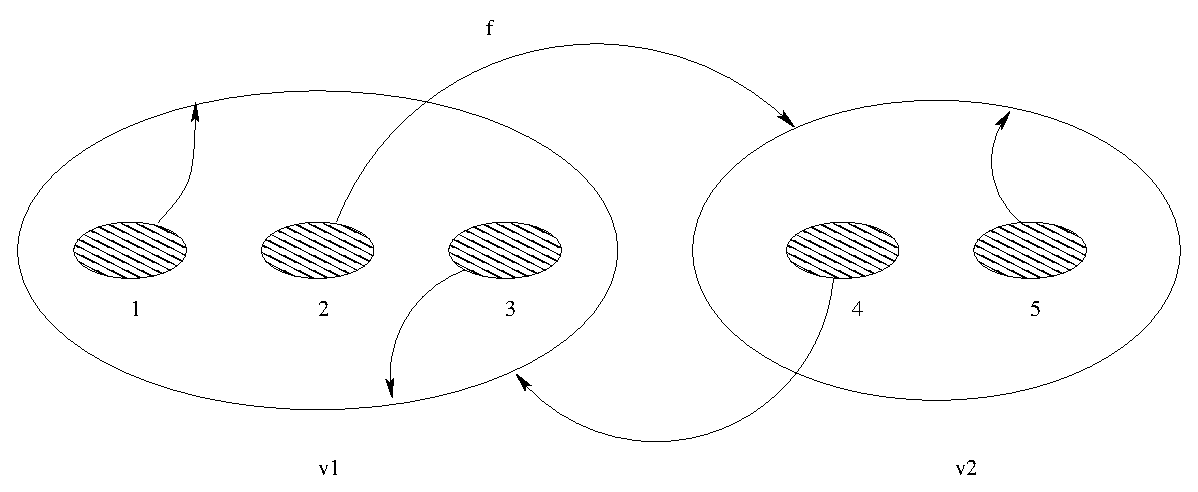
\includegraphics[scale=0.55]{cantor1.eps}
    %  note that the square brace option below is only required
    %  if you intend to produce a list of illustrations
    \caption[Shortened figure caption for the list of illustrations]
      {A Cantor repeller. Long figure captions will be indented left
      and right; short ones will be centred by default.}
    \label{cantor}
\rule[-20pt]{\textwidth}{0.6pt}
\begin{verbatim}
  \begin{figure}
    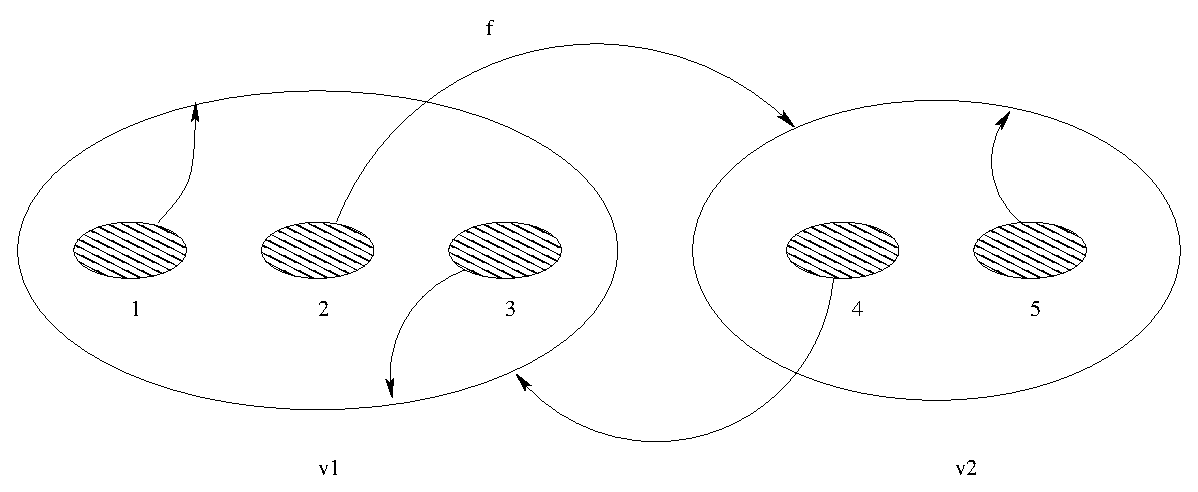
\includegraphics[scale=0.55]{cantor1.eps}
    %  note that the square brace option below is only required
    %  if you intend to produce a list of illustrations
    \caption[Shortened figure caption for the list of illustrations]
      {A Cantor repeller. Long figure captions will be indented left
      and right; short ones will be centred by default.}
    \label{cantor}
  \end{figure}
\end{verbatim}
\rule[20pt]{\textwidth}{0.5pt}
  \end{figure}

\section{Tables}

The \cambridge\ class will cope with most positioning of your tables. Table captions must be included first, the the label, then the body of the table. This is illustrated in Table~\ref{sample-table}.
  \begin{table}
    \begin{minipage}{188pt}
      %  note that the square brace option below is only required
      %  if you intend to produce a list of tables
    \caption[Shortened table caption for the list of tables]
      {Longer table captions have to be placed inside
      a minipage, otherwise they overhang the table rules.}
    \label{sample-table}
    \addtolength\tabcolsep{2pt}% to stretch columns, if required
      \begin{tabular}{@{}c@{\hspace{25pt}}ccc@{}}
        \hline \hline
        Figure\footnote{\textit{Note:} You must also use a minipage
          environment if you have footnotes.} & $hA$ & $hB$ & $hC$\\
        \hline
        1 & $\exp\left(\pi i\frac58\right)$
          & $\exp\left(\pi i\frac18\right)$ & $0$\\[3pt]
        2 & $-1$    & $\exp\left(\pi i\frac34\right)$ & $1$\\[11pt]
        3 & $-4+3i$ & $-4+3i$ & $\frac74$\\[3pt]
        4 & $-2$    & $-2$    & $\frac54 i$ \\
        \hline \hline
      \end{tabular}
    \end{minipage}
    \rule[-20pt]{\textwidth}{0.5pt}
\begin{verbatim}
  \begin{table}
    \begin{minipage}{188pt}
      %  note that the square brace option below is only required
      %  if you intend to produce a list of tables
    \caption[Shortened table caption for the list of tables]
      {Longer table captions have to be placed inside
      a minipage, otherwise they overhang the table rules.}
    \label{sample-table}
    \addtolength\tabcolsep{2pt}% to stretch columns, if required
      \begin{tabular}{@{}c@{\hspace{25pt}}ccc@{}}
        \hline \hline
        Figure\footnote{\textit{Note:} You must also use a minipage
          environment if you have footnotes.} & $hA$ & $hB$ & $hC$\\
        \hline
        1 & $\exp\left(\pi i\frac58\right)$
          & $\exp\left(\pi i\frac18\right)$ & $0$\\[3pt]
        2 & $-1$    & $\exp\left(\pi i\frac34\right)$ & $1$\\[11pt]
        3 & $-4+3i$ & $-4+3i$ & $\frac74$\\[3pt]
        4 & $-2$    & $-2$    & $\frac54 i$ \\
        \hline \hline
      \end{tabular}
    \end{minipage}
  \end{table}
\end{verbatim}
\rule[20pt]{\textwidth}{0.5pt}
  \end{table}

\subsection{My vertical rules have disappeared}

Vertical rules in tables are not \cambridge\ style, and have been automatically removed; this gives your document a truly professional look. Instead of vertical rules, we recommend the use of extra horizontal space, see Section~\ref{addhoriz}. The rules have been removed by redefining the \verb"tabular" environment. The amended definition also inserts extra vertical space above and below the horizontal rules (produced by \verb"\hline").

If you really must have them reinstated, read Section~\ref{reinstate}.

\subsection{Reinstating the vertical rules}
\label{reinstate}
Authors can revert to the standard \LaTeX\ style, if necessary. Tables will take on a rather squashed appearance, as in the \LaTeX\ book, whereby there is no added space around horizontal rules. Add the command \verb"\reinstaterules" in the preamble, and re-run your files through \LaTeX.

\subsection{There is very little space around the rules in my~table}
Tables revert to the standard, rather squashed look of standard \LaTeX\ tables for two reasons:
\begin{enumerate}
  \item you are using \verb"array.sty"; or
  \item you have chosen to reinstate vertical rules (see Section~\ref{reinstate})
\end{enumerate}
In both cases, the tabular environment is redefined.


\subsection{Adding space between columns}
\label{addhoriz}
You can add space (2pt in this example) between every column using\linebreak \verb"\addtolength\tabcolsep{2pt}". However, if you only wanted to expand the space between columns~1 and~2 to~25pt, you would do this using\linebreak  \verb"\begin{tabular}{@{}c@{\hspace{25pt}}ccc@{}}" (see Table~\ref{sample-table}).

\subsection{Adding space between rows}
If you need some form of separation between rows (for example, between rows~2 and~3 in the body of Table~\ref{sample-table}), adding \verb"[11pt]" immediately after the double backslash at the end of row~2 will add an 11pt vertical space (the equivalent of a blank line at this typesize). This is neater than adding another horizontal line.


\section{Landscape figures and tables, using rotating.sty}

Landscape figures and tables (floats) may be typeset using the \verb"rotating.sty" package. Note that the direction of rotation depends on the page number -- which requires at least two passes through \LaTeX. If we are going to know whether pages are odd or even, we need to use the \verb"\pageref" mechanism, and labels. But labels won't work unless the user has put in a caption. \textit{Beware!}

In addition to \verb"rotating.sty", you should also include \verb"floatpag.sty" and the command \verb"\rotfloatpagestyle{empty}". This combination ensures that headers and footers are removed from the float page:
\begin{verbatim}
  \usepackage{rotating}
  \usepackage{floatpag}
  \rotfloatpagestyle{empty}
\end{verbatim}
In some DVI previewers, floats may not appear rotated. If this happens, you need to convert the DVI file to PostScript or PDF.

Occasionally, when you convert a PostScript file to a PDF file, you may find that the page comes out upside-down. There will be a setting to change this. For instance, if you are using PDFCreator 0.9.7, choose the following options in this sequence:
\begin{description}
  \item Options -- Program -- PDF -- Auto-Rotate Pages: Change to `None'.
\end{description}
Other programs will have similar\vadjust{\pagebreak} procedures.


\subsection{Coding for landscape figures}

The landscape figure (Figure~\ref{sidecantor}) was typeset using the following coding:
\begin{verbatim}
  \begin{sidewaysfigure}
    \centering
    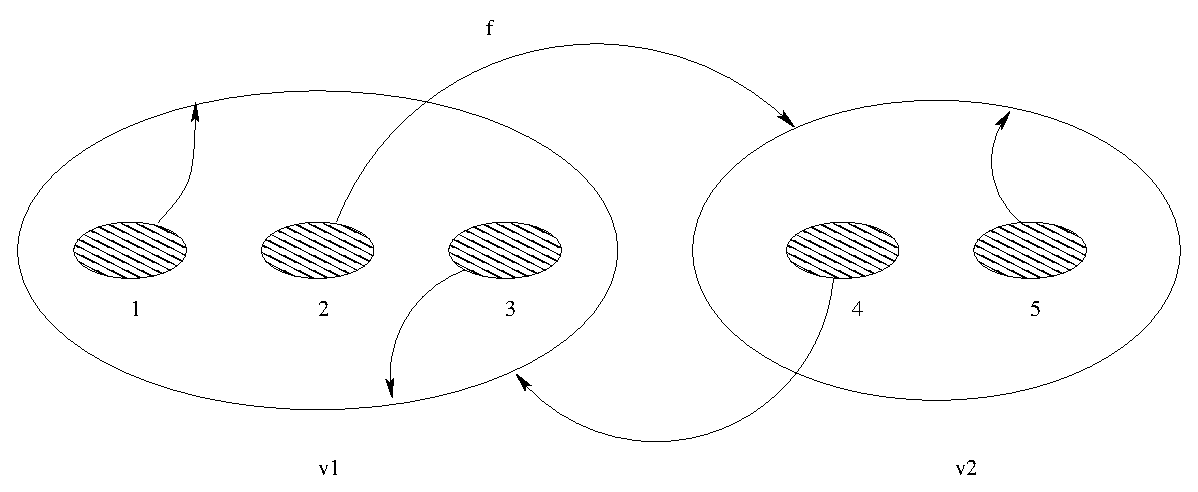
\includegraphics[scale=0.95]{cantor1.eps}
    %  note that the square brace option below is only required
    %  if you intend to produce a list of illustrations
    \caption[Landscape figure]{A Cantor repeller. Figure captions
      will be centred by default.}
    \label{sidecantor}
  \end{sidewaysfigure}
\end{verbatim}
  \begin{sidewaysfigure}
    \centering
    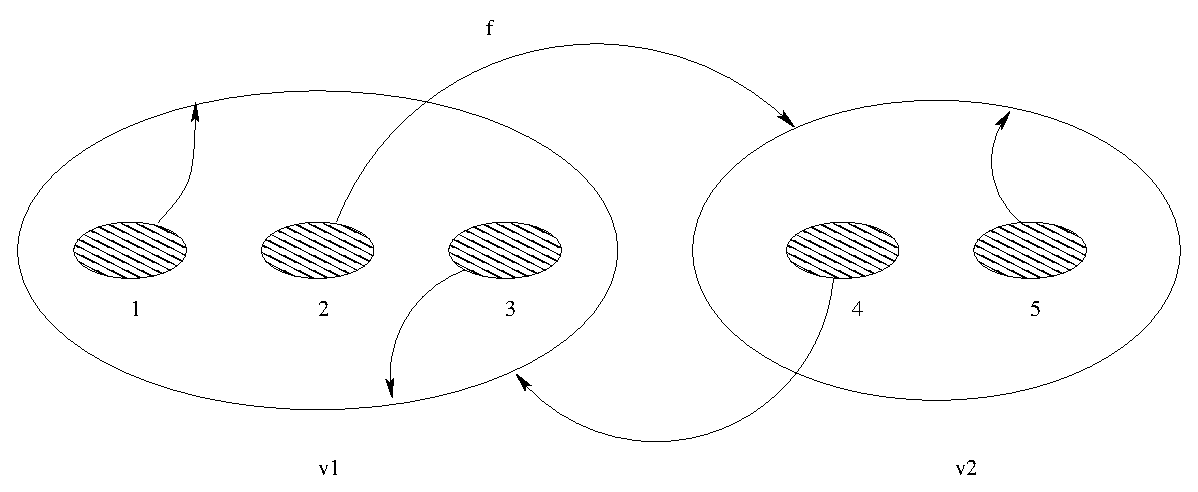
\includegraphics[scale=0.95]{cantor1.eps}
    %  note that the square brace option below is only required
    %  if you intend to produce a list of illustrations
    \caption[Landscape figure]{A Cantor repeller. Figure captions
      will be centred by default.}
    \label{sidecantor}
  \end{sidewaysfigure}



\subsection{Coding for landscape tables}

Table~\ref{sideways} has been produced using the following coding:
%
\begin{smallverbatim}
\begin{sidewaystable}
  \caption[Landscape table]{Grooved ware and beaker features, their finds and
    radiocarbon dates. For a breakdown of the pottery assemblages see
    Tables~I and~III; for the flints see Tables~II and~IV; for the animal
    bones see Table~V.}
  \label{sideways}
  \addtolength\tabcolsep{-2pt}
  \begin{tabular}{@{}lcccllccccc@{}}
  \hline\hline
  Context & Length & Breadth/  & Depth & Profile & Pottery & Flint & Animal
                                                   & Stone & Other & C14 Dates\\
  && Diameter &&&&& Bones\\[5pt]
  & m & m & m\\
  \hline\\[-5pt]
  \multicolumn{10}{@{}l}{\textbf{Grooved Ware}}\\
  784 & --   & 0.9$\phantom{0}$ &0.18  & Sloping U & P1      & $\times$46
        & $\phantom{0}$$\times$8 && $\times$2 bone & 2150 $\pm$100\,\textsc{bc}\\
  785 & --   & 1.00             &0.12   & Sloping U & P2--4  & $\times$23
                                           & $\times$21 & Hammerstone & -- & --\\
  962 & --   & 1.37             &0.20   & Sloping U & P5--6  & $\times$48
                     & $\times$57 & --& --& 1990 $\pm$80\,\textsc{bc} (Layer 4)\\
  &&&&&&&&&& 1870 $\pm$90\,\textsc{bc} (Layer 1)\\
  983 & 0.83 & 0.73             &0.25   & Stepped U & --     & $\times$18
                                & $\phantom{0}$$\times$8 & -- & Fired clay & --\\
  &&&&&&&&&&\\
  \multicolumn{10}{@{}l}{\textbf{Beaker}}\\
  552 & --   & 0.68             & 0.12  & Saucer    & P7--14 & --           & --
                                                                   & -- &-- &--\\
  790 & --   & 0.60             & 0.25  & U         & P15    & $\times$12   & --
                                                      & Quartzite-lump & -- &--\\
  794 & 2.89 & 0.75             & 0.25  & Irreg.    & P16    & $\phantom{0}$$\times$3
                                                              & -- & -- &-- &--\\
  \hline\hline
  \end{tabular}
\end{sidewaystable}
\end{smallverbatim}
%
\begin{sidewaystable}
  \caption[Landscape table]{Grooved ware and beaker features, their finds and
    radiocarbon dates. For a breakdown of the pottery assemblages see
    Tables~I and~III; for the flints see Tables~II and~IV; for the animal
    bones see Table~V.}
  \label{sideways}
  \addtolength\tabcolsep{-2pt}
  \begin{tabular}{@{}lcccllccccc@{}}
  \hline\hline
  Context & Length & Breadth/  & Depth & Profile & Pottery & Flint & Animal
                                                   & Stone & Other & C14 Dates\\
  && Diameter &&&&& Bones\\[5pt]
  & m & m & m\\
  \hline\\[-5pt]
  \multicolumn{10}{@{}l}{\textbf{Grooved Ware}}\\
  784 & --   & 0.9$\phantom{0}$ &0.18  & Sloping U & P1      & $\times$46
        & $\phantom{0}$$\times$8 && $\times$2 bone & 2150 $\pm$100\,\textsc{bc}\\
  785 & --   & 1.00             &0.12   & Sloping U & P2--4  & $\times$23
                                           & $\times$21 & Hammerstone & -- & --\\
  962 & --   & 1.37             &0.20   & Sloping U & P5--6  & $\times$48
                     & $\times$57 & --& --& 1990 $\pm$80\,\textsc{bc} (Layer 4)\\
  &&&&&&&&&& 1870 $\pm$90\,\textsc{bc} (Layer 1)\\
  983 & 0.83 & 0.73             &0.25   & Stepped U & --     & $\times$18
                                & $\phantom{0}$$\times$8 & -- & Fired clay & --\\
  &&&&&&&&&&\\
  \multicolumn{10}{@{}l}{\textbf{Beaker}}\\
  552 & --   & 0.68             & 0.12  & Saucer    & P7--14 & --           & --
                                                                   & -- &-- &--\\
  790 & --   & 0.60             & 0.25  & U         & P15    & $\times$12   & --
                                                      & Quartzite-lump & -- &--\\
  794 & 2.89 & 0.75             & 0.25  & Irreg.    & P16    & $\phantom{0}$$\times$3
                                                              & -- & -- &-- &--\\
  \hline\hline
  \end{tabular}%
\end{sidewaystable}

\endinput% features of the \cambridge\ class file
  % chap3.tex
% 2010/09/09, v2.10

\chapter{Mathematical solutions}
\label{mathsol}

\section{Why are we using amsthm.sty?}

Many authors are already using this style file, so we have decided that rather than re-invent the wheel, we will make it part of our distribution. This means that at the top of the root file must include the following lines:\\[0.5\baselineskip]
\verb"  \documentclass{"\texttt{\cambridge}\verb"}"\\
\verb"  \usepackage{amsmath}"\\
\verb"  \usepackage{amsthm}"\\[0.5\baselineskip]
As mentioned in Chapter~\ref{intro}, if your book does not use theorems, proofs, etc., then there is no need to include the amsthm package, but you do need to include these files to run this guide through \LaTeX. Note that if you are also using \verb"amsmath.sty", it \emph{must} precede \verb"amsthm.sty".

The instructions for amsthm.sty are documentated separately in \texttt{amsthdoc.pdf}. We are including \texttt{amsthm.sty} and \texttt{amsthdoc.pdf} in this distribution for your convenience, but you may find more recent versions on the web. The following sections discuss the basic features, plus a few extras.

To save time, you may cut and paste the code in Appendix~\ref{amsthmcommands} into your root file. This is a comprehensive (but not necessarily a complete) list of theorem-like environments you may wish to use.

The \verb"amsthm" commands used in this guide are detailed in Appendix~\ref{rootfile}. They are simply a subset of commands from Appendix~\ref{amsthmcommands}; some illustrate unnumbered versions.

Please note that theorems, definitions, remarks, etc.\ should be numbered in a single sequence, either by chapter (Chapter~4 would have Definition~4.1, Lemma~4.2, Lemma~4.3, Proposition~4.4, Corollary~4.5) or by section (Definition~4.1.1, Lemma~4.1.2, Lemma~4.1.3, Proposition~4.1.4, Corollary~4.1.5).

To number these elements by chapter in this guide, we have used\linebreak \verb"\newtheorem{theorem}{Theorem}[chapter]". If you prefer to have the elements numbered by section, replace \verb"[chapter]" with \verb"[section]".

\section{amsthm styles}

If no \verb"\theoremstyle" command is given, the style used will be \texttt{plain}. To specify different styles, divide your \verb"\newtheorem" commands into groups and preface each group with the appropriate \verb"\theoremstyle".

\subsection{amsthm {\upshape\texttt{plain}} style}

The \texttt{plain} style is normally used for theorems, lemmas, corollaries, propositions, conjectures, criterion and algorithms. Authors are free to define their preferred numbering systems for these. The following example resets the theorem numbers for each chapter; lemmas follow in the same sequence. We have also requested that corollaries remain unnumbered by using the starred version:
\begin{verbatim}
  \theoremstyle{plain}% default
  \newtheorem{theorem}{Theorem}[chapter]
  \newtheorem{lemma}[theorem]{Lemma}
  \newtheorem*{corollary}{Corollary}

  \begin{theorem}
    Let the scalar function\ldots
  \end{theorem}
  \begin{lemma}[Tranah]
    The first-order free surface amplitudes\ldots
  \end{lemma}
  \begin{lemma}[\citealp{MenshEst}]
    The exotic behaviours of Lagrangian\ldots
  \end{lemma}
  \begin{corollary}
    Let $G$ be the free group on\ldots
  \end{corollary}
\end{verbatim}
will produce the following output:
  \begin{theorem}
    Let the scalar function\ldots
  \end{theorem}
  \begin{lemma}[Tranah]
    The first-order free surface amplitudes\ldots
  \end{lemma}
  \begin{lemma}[\citealp{MenshEst}]
    The exotic behaviours of Lagrangian\ldots
  \end{lemma}
  \begin{corollary}
    Let $G$ be the free group on\ldots
  \end{corollary}
%
Note that Corollaries would normally be in the same numbering sequence as Theorems and Lemmas. If you'd prefer your theorems to be typeset in roman (though this is not recommended) use the amsthm \texttt{definition} style instead (see Section~\ref{amsdefn}).

\subsection{amsthm {\upshape\texttt{definition}} style}
\label{amsdefn}

The \texttt{definition} style is normally used for definitions, conditions, problems, examples. It may also be used to set up Exercises (see Appendix~\ref{amsthmcommands} for an example), although the \verb"{exerciselist}" environment described in Section~\ref{exendofsections} does the equivalent.  Again, authors are free to define their preferred numbering systems for these. However, it is most usual to continue with the same numbering sequence as for Theorems, Lemmas, etc.:
\begin{verbatim}
  \theoremstyle{definition}
  \newtheorem{definition}[theorem]{Definition}
  \newtheorem{example}[theorem]{Example}

  \begin{definition}
    The series above is the Green function\ldots
  \end{definition}
  \begin{definition}
    The correlation between the real and estimated flow\ldots
  \end{definition}
  \begin{example}
    Consider spatial and temporal problems\ldots
  \end{example}
\end{verbatim}
will produce the following output:
  \begin{definition}
    The series above is the Green function\ldots
  \end{definition}
  \begin{definition}
    The correlation between the real and estimated flow\ldots
  \end{definition}
  \begin{example}
    Consider spatial and temporal problems\ldots
  \end{example}


\subsection{amsthm {\upshape\texttt{remark}} style}
The \texttt{remark} style is normally used for remarks, notes, notation, claims, summary, acknowledgements, cases, conclusions. Again, authors are free to define their preferred numbering systems for these.
\begin{verbatim}
  \theoremstyle{remark}
  \newtheorem*{remark}{Remark}
  \newtheorem*{case}{Case}

  \begin{remark}
    The absolute amplitude of a stratified wake\ldots
  \end{remark}
  \begin{case}
    The profiles of quadratic fluctuations\ldots
  \end{case}
\end{verbatim}
will produce the following output:
  \begin{remark}
    The absolute amplitude of a stratified wake\ldots
  \end{remark}
  \begin{case}
    The profiles of quadratic fluctuations\ldots
  \end{case}

\section{Proofs}
\label{proofs}

The \verb"proof" environment is also part of the amsthm package, and provides a consistent format for proofs.
 For example,
\begin{verbatim}
  \begin{proof}
    Use $K_\lambda$ and $S_\lambda$ to translate combinators
    into $\lambda$-terms. For the converse, translate
    $\lambda x$ \ldots by [$x$] \ldots and use induction
    and the lemma.
  \end{proof}
\end{verbatim}
produces the following:
  \begin{proof}
    Use $K_\lambda$ and $S_\lambda$ to translate combinators
    into $\lambda$-terms. For the converse, translate
    $\lambda x$ \ldots by [$x$] \ldots and use induction
    and the lemma.
  \end{proof}

\subsection{Changing the word `Proof' to something else}

An optional argument allows you to substitute a different name for the standard `Proof'. To change the proof heading to read `Proof of the Pythagorean Theorem', key the following:
\begin{verbatim}
  \begin{proof}[Proof of the Pythagorean Theorem]
    Start with a generic right-angled triangle\ldots
  \end{proof}
\end{verbatim}
which produces:
  \begin{proof}[Proof of the Pythagorean Theorem]
    Start with a generic right-angled triangle\ldots
  \end{proof}


\subsection{Typesetting a proof without a \qedsymbol}

This is not part of the amsthm package. Use the \verb"proof*" version. For example,
\begin{verbatim}
  \begin{proof*}
    The apparent virtual mass coefficient\ldots
  \end{proof*}
\end{verbatim}
produces the following:
  \begin{proof*}
    The apparent virtual mass coefficient\ldots
  \end{proof*}

\subsection{Placing the \qedsymbol\ after a displayed equation}

To avoid the \qedsymbol\ dropping onto the following line at the end of a proof,
\begin{verbatim}
  \begin{proof}
    \ldots and, as we are all aware,
    \[
       E=mc^2. \qedhere
    \]
  \end{proof}
\end{verbatim}
produces the following:
  \begin{proof}
    \ldots and, as we are all aware,
    \[
       E=mc^2. \qedhere
    \]
  \end{proof}
When used with the amsmath package, version~2 or later, \verb"\qedhere" will position \qedsymbol\ flush right; with earlier versions, \qedsymbol\ will be spaced a quad away
from the end of the text or display.

If \verb"\qedhere" produces an error message in an equation, try using \verb"\mbox{\qedhere}" instead.

\subsection{Placing the \qedsymbol\ after a displayed eqnarray}

This is also not part of the amsthm package. To enable this, you need to used the starred version of \verb"proof", and add both \verb"\arrayqed" and \verb"\arrayqedhere", as shown in the following example:
\begin{verbatim}
  \begin{proof*}
    The following equations prove the theorem:
      \arrayqed
        \begin{eqnarray}
          \epsilon &=& -\frac{1}{2}U_0\frac{\mathrm{d}q'^2}
                       {\mathrm{d}x}\nonumber\\
                   &=& 10\nu\frac{q'^2}{\lambda^2}
        \arrayqedhere
        \end{eqnarray}
  \end{proof*}
\end{verbatim}
produces the following:
  \begin{proof*}
    The following equations prove the theorem:
      \arrayqed
        \begin{eqnarray}
          \epsilon &=& -\frac{1}{2}U_0\frac{\mathrm{d}q'^2}
                       {\mathrm{d}x}\nonumber\\
                   &=& 10\nu\frac{q'^2}{\lambda^2}
        \arrayqedhere
        \end{eqnarray}
  \end{proof*}

\endinput
% mathematical solutions

  \part{Closing features}
  % chap4.tex
% 2010/09/09, v2.10

\chapter{Reference and bibliography lists}

\section{Automatic lists using \textsc{Bib}\upshape{\TeX}}

We have chosen to use the natbib package because of its versatility.

First, call in \texttt{natbib.sty}. If you are using the multi-contributor option, you will get an unnumbered section heading, otherwise it will be an unnumbered chapter heading.

The bibliography file for this guide (\texttt{\cambridge guide.tex}) is called \texttt{percolation.bib}; the bibliography style is \texttt{cambridgeauthordate.bst}, so place the final two commands at the point where you would like the references to appear:
%
\begin{verbatim}
    \usepackage{natbib}
      :
  % \renewcommand{\refname}{Bibliography}
    \bibliography{percolation}
    \bibliographystyle{cambridgeauthordate}
\end{verbatim}
%
Note that if you uncomment the third line shown above, you can change the heading from `References' to `Bibliography'. Next, \LaTeX\ your book twice. Then run \textsc{Bib}\TeX\ by executing the command\\[0.5\baselineskip]
\verb"  bibtex "\texttt{\cambridge guide}\\[0.5\baselineskip]
Finally, run your book through \LaTeX\ twice again. This series of runs will generate a file called \texttt{\cambridge guide.bbl}, which will then be included by \verb"\bibliography{percolation}".

Suppose you have cited 8 entries from the `percolation' database, e.g. \verb"\citealp{MenshEst}"; \verb"\citealp{Kasymp}"; \verb"\citealp{VGFH}"; \verb"\citealp{HamMaz94}"; \verb"\citealp{HamLower}"; \verb"\citealp{AiBar87}"; \verb"\citealp{MMS}"; and \verb"\citealp{HamAtomBond}"; the output will be just those 8~entries (see page~\pageref{refs}).%
% add these entries to the list without referring to them
\nocite{MenshEst}\nocite{Kasymp}\nocite{VGFH}\nocite{HamMaz94}\nocite{HamLower}\nocite{AiBar87}\nocite{MMS}\nocite{HamAtomBond}

\section{Citations using natbib commands}
Here are some of the basic citation commands available with the natbib package; there are many more if you cannot find what you need in this list. Bear in mind that Menshikov (1985) or (Menshikov, 1985) read best, depending on context.\\*[0.5\baselineskip]
\begin{tabular}{@{}ll@{}}
\verb"\citep{MenshEst}"
    & $\rightarrow\enskip$\citep{MenshEst}\\
\verb"\citep[see][p.$\,$34]{MenshEst}"
    & $\rightarrow\enskip$\citep[see][p.$\,$34]{MenshEst}\\
\verb"\citep[e.g.][]{MenshEst}"
    & $\rightarrow\enskip$\citep[e.g.][]{MenshEst}\\
\verb"\citep[Section~2.3]{MenshEst}"
    & $\rightarrow\enskip$\citep[Section~2.3]{MenshEst}\\
\verb"\citep{MenshEst, VGFH}"\\
    & $\hspace{-70pt}\rightarrow\enskip$\citep{MenshEst, VGFH}\\
\verb"\cite{MenshEst, VGFH}"\\
    & $\hspace{-70pt}\rightarrow\enskip$\cite{MenshEst, VGFH}\\
\verb"\citealt{MenshEst}"
    & $\rightarrow\enskip$\citealt{MenshEst}\\
\verb"\cite{MenshEst}"
    & $\rightarrow\enskip$\cite{MenshEst}\\
\verb"\citealp{MenshEst}"
    & $\rightarrow\enskip$\citealp{MenshEst}\\
\verb"\citeauthor{MenshEst}"
    & $\rightarrow\enskip$\citeauthor{MenshEst}\\
\verb"\citeyearpar{MenshEst}"
    & $\rightarrow\enskip$\citeyearpar{MenshEst}\\
\verb"\citeyear{MenshEst}"
    & $\rightarrow\enskip$\citeyear{MenshEst}
\end{tabular}


\section{How to change reference entries from author--date to~numbers}
\label{numberedbiblio}

\LaTeX\ authors are used to \verb"\cite{...}" producing a reference such as~[11] in their manuscripts. If you prefer this style, it is an option within the natbib package:
\begin{verbatim}
  \usepackage[numbers]{natbib}
\end{verbatim}

\section{Keying in your reference list for an author--date system}
\label{authordatebiblio}

The entries need to be keyed as below. Note that if you uncomment the first line, you can change the heading from `References' to `Bibliography':
%
\begin{smallverbatim}
% \renewcommand{\refname}{Bibliography}
  \begin{thebibliography}{8}
    \expandafter\ifx\csname natexlab\endcsname\relax
      \def\natexlab#1{#1}\fi
    \expandafter\ifx\csname selectlanguage\endcsname\relax
      \def\selectlanguage#1{\relax}\fi

  \bibitem[Aizenman and Barsky, 1987]{AiBar87}
    Aizenman, M., and Barsky, D.~J. 1987.
    Sharpness of the phase transition in percolation models.
    {\em Comm. Math. Phys.}, {\bf 108}, 489--526.

  \bibitem[Hammersley, 1957]{HamLower}
    Hammersley, J.~M. 1957.
    Percolation processes: Lower bounds for the critical probability.
    {\em Ann. Math. Statist.}, {\bf 28}, 790--795.

  \bibitem[Hammersley, 1961]{HamAtomBond}
    Hammersley, J.~M. 1961.
    Comparison of atom and bond percolation processes.
    {\em J. Mathematical Phys.}, {\bf 2}, 728--733.

  \bibitem[Hammersley and Mazzarino, 1994]{HamMaz94}
    Hammersley, J.~M., and Mazzarino, G. 1994.
    Properties of large Eden clusters in the plane.
    {\em Combin. Probab. Comput.}, {\bf 3}, 471--505.

  \bibitem[Kesten, 1990]{Kasymp}
    Kesten, H. 1990.
    Asymptotics in high dimensions for percolation.
    Pages  219--240 of: Grimmett, G.~R., and Welsh, D.~J.~A. (eds),
    {\em Disorder in Physical Systems: A Volume in Honour of John Hammersley}.
    Oxford University Press.

  \bibitem[Menshikov, 1985]{MenshEst}
    Menshikov, M.~V. 1985.
    Estimates for percolation thresholds for lattices in {${\bf R}\sp n$}.
    {\em Dokl. Akad. Nauk SSSR}, {\bf 284}, 36--39.

  \bibitem[Menshikov et~al., 1986]{MMS}
    Menshikov, M.~V., Molchanov, S.~A., and Sidorenko, A.~F. 1986.
    Percolation theory and some applications.
    Pages  53--110 of: {\em Probability theory. Mathematical
    statistics. Theoretical cybernetics, Vol. 24 (Russian)}.
    Akad. Nauk SSSR Vsesoyuz. Inst. Nauchn. i Tekhn. Inform.
    Translated in {\em J. Soviet Math}. {\bf 42} (1988), no. 4,
    1766--1810.

  \bibitem[Vyssotsky et~al., 1961]{VGFH}
    Vyssotsky, V.~A., Gordon, S.~B., Frisch, H.~L., and Hammersley, J.~M. 1961.
    Critical percolation probabilities (bond problem).
    {\em Phys. Rev.}, {\bf 123}, 1566--1567.

  \end{thebibliography}
\end{smallverbatim}

\section{Keying in your reference list for a numbered system}

For this style, you may omit the optional square brace shown in Section~\ref{authordatebiblio}. Once again, if you uncomment the first line, you can change the heading from `References' to `Bibliography':
%
\begin{smallverbatim}
% \renewcommand{\refname}{Bibliography}
  \begin{thebibliography}{8}

  \bibitem{AiBar87}
    Aizenman, M., and Barsky, D.~J. 1987.
    Sharpness of the phase transition in percolation models.
    {\em Comm. Math. Phys.}, {\bf 108}, 489--526.

  \bibitem{HamLower}
    Hammersley, J.~M. 1957.
    Percolation processes: Lower bounds for the critical probability.
    {\em Ann. Math. Statist.}, {\bf 28}, 790--795.

  \bibitem{HamAtomBond}
    Hammersley, J.~M. 1961.
    Comparison of atom and bond percolation processes.
    {\em J. Mathematical Phys.}, {\bf 2}, 728--733.
      :
      :
  \bibitem[Vyssotsky et~al., 1961]{VGFH}
    Vyssotsky, V.~A., Gordon, S.~B., Frisch, H.~L., and Hammersley, J.~M. 1961.
    Critical percolation probabilities (bond problem).
    {\em Phys. Rev.}, {\bf 123}, 1566--1567.

  \end{thebibliography}
\end{smallverbatim}

\endinput% references and bibliographies
  % chap5.tex
% 2010/09/09, v2.10

\chapter{Indexes}
\label{indexes}

\section{Creating a single index using makeidx.sty}
To generate a single index, normally a subject index, the commands would take the form:
\begin{verbatim}
  \index{diffraction}
  \index{force!hydrodynamic}
  \index{force!interactive}
\end{verbatim}
  %\index{diffraction}%
  %\index{force!hydrodynamic}%
  %\index{force!interactive}%
The following commands are then required in the preamble:
\begin{verbatim}
  \usepackage{makeidx}
  \makeindex
\end{verbatim}
and at the point you wish your index to appear,
\begin{verbatim}
  \printindex
\end{verbatim}
Run your book through \LaTeX\ enough times so that the labels, etc., are stable. Then execute the command:\\[0.5\baselineskip]
\verb"  makeindex "\texttt{\cambridge guide}\\[0.5\baselineskip]
To include the index, you need to run \LaTeX\ one more time.


\section{Creating multiple indexes using multind.sty}
This guide has been prepared using \verb"multind.sty". This style file redefines the \verb"\makeindex", \verb"\index" and \verb"\printindex" commands to deal with multiple indexes.

Suppose you want to create an author index and a subject index. The entries should be in the text as usual, but take the following form:
\begin{verbatim}
  \index{authors}{Young, P.D.F.}
  \index{authors}{Tranah, D.A.}
  \index{authors}{Peterson, K.}
  \index{subject}{diffraction}
  \index{subject}{force!hydrodynamic}
  \index{subject}{force!interactive}
\end{verbatim}
  \index{authors}{Young, P.D.F.}%
  \index{authors}{Tranah, D.A.}%
  \index{authors}{Peterson, K.}%
  \index{subject}{diffraction}%
  \index{subject}{force!hydrodynamic}%
  \index{subject}{force!interactive}%
In the preamble, you need to add the following lines:
\begin{verbatim}
  \usepackage{multind}\ProvidesPackage{multind}
  \makeindex{authors}
  \makeindex{subject}
\end{verbatim}
It is crucial to add the command \verb"\ProvidesPackage{multind}"; this will send a message to the class file to re-style the index into the \cambridge\ style. You will get a warning in your log file:
\begin{verbatim}
  LaTeX Warning: You have requested package `',
                 but the package provides `multind'.
\end{verbatim}
which can be ignored. At the point where you wish your indexes to appear, you then need the commands:
\begin{verbatim}
  \printindex{authors}{Author index}
  \printindex{subject}{Subject index}
\end{verbatim}
Run your book through \LaTeX\ enough times so that the labels, etc., are stable. Then execute the commands:
\begin{verbatim}
  makeindex authors
  makeindex subject
\end{verbatim}
To include the indexes, you need to run \LaTeX\ one more time.

\section{Creating multiple indexes using index.sty}

This style file allows you to define new indexes. Suppose you want to create an author index as well as a normal subject index. The entries should be in the text as usual, but take the following form:
\begin{verbatim}
  \index[aut]{Young, P.D.F.}
  \index[aut]{Tranah, D.A.}
  \index[aut]{Peterson, K.}
  \index{diffraction}
  \index{force!hydrodynamic}
  \index{force!interactive}
\end{verbatim}
  %\index[aut]{Young, P.D.F.}%
  %\index[aut]{Tranah, D.A.}%
  %\index[aut]{Peterson, K.}
  %\index{diffraction}%
  %\index{force!hydrodynamic}%
  %\index{force!interactive}%
To create the extra author index, you need to have the following lines in the preamble:
\begin{verbatim}
  \usepackage{index}
  \makeindex
  \newindex{aut}{adx}{and}{Author index}
\end{verbatim}
At the point where you wish your indexes to appear, use:
\begin{verbatim}
  \printindex[aut]
  \printindex
\end{verbatim}
Run your book through \LaTeX\ enough times so that the labels, etc., are stable. Then execute the commands:\\[0.5\baselineskip]
\verb"  makeindex -o "\texttt{\cambridge guide.and \cambridge guide.adx}\\
\verb"  makeindex "\texttt{\cambridge guide}\\[0.5\baselineskip]
To include the indexes, you need to run \LaTeX\ one more time.

\subsection{Caution -- from the authors of index.sty}

In order to implement \verb"index.sty", it's been necessary to modify a number of \LaTeX\ commands seemingly unrelated to indexing, namely, \verb"\@starttoc", \verb"\raggedbottom", \verb"\flushbottom", \verb"\addcontents", \verb"\markboth", and \verb"\markright". Naturally, this could cause incompatibilities between \texttt{index.sty} and any style files that either redefine these same commands or make specific assumptions about how they operate.

The redefinition of \verb"\@starttoc" is particularly bad, since it introduces an incompatibility with the AMS document classes. This will be addressed soon.

In the current implementation, \texttt{index.sty} uses one output stream for each index.  Since there are a limited number of output indexes, this means that there is a limit on the number of indexes you can have in a document.  There is more information on this in \verb"index.dtx" which is part of the \verb"index.sty" distribution.\\[\baselineskip]
%
\textit{For these reasons, whilst all care has been taken to deal with these changes in \cambridge.cls, if you do find incompatibilities with other files, please contact us at texline@cambridge.org with your source files, class and style files, and log file.}

\endinput
% single and multiple indexes

  \backmatter
% if you only have one appendix, use \oneappendix instead of \appendix
  \appendix
  % appendixA.tex
% 2010/09/09, v2.10

\chapter{Typesetting appendices}

\section{Single-contributor books}
\subsection{How to typeset one appendix}
If you have just one appendix, say \verb"appendix.tex", you will want to generate a chapter head `Appendix' rather than `Appendix A'. Use \verb"\oneappendix" in the main file, as follows:
\begin{verbatim}
  \oneappendix
  \include{appendix}
\end{verbatim}

\subsection{How to typeset several appendices}
The coding used to generate the appendices in this guide is as follows:
\begin{verbatim}
  \appendix
  \include{appendixA}
  \include{appendixB}
  \include{appendixC}
\end{verbatim}

\section{Multi-contributor books}

\subsection{How to typeset one appendix}
If you have just one appendix, it will be the next section head and you should include the following code at the end of your chapter:
\begin{verbatim}
  \oneappendix
  \section{Appendix heading}
  \subsection{Subheading}
  \endappendix
\end{verbatim}
You will need to add \verb"\endappendix" if you have further section heads in this chapter.


\subsection{How to typeset several appendices}
The following code will genenerate Appendix~A and Appendix~B at the end of your chapter:
\begin{verbatim}
  \appendix
  \section{Appendix heading}
  \subsection{Subheading}
    :
  \section{Next appendix heading}
  \subsection{Next subheading}
  \endappendix
\end{verbatim}
Again, you will need to add \verb"\endappendix" if you have further section heads in this chapter.

\section{Numbering systems}

Equations in appendices will be numbered as follows:
\begin{equation}
  E=mc^2,
\end{equation}
and figure captions as follows:
\begin{figure}[h]
\caption[Similarity solutions]{Similarity solutions.}
\end{figure}

\endinput
  % appendixB.tex
% 2010/09/09, v2.10

\chapter{amsthm commands}
\label{amsthmcommands}

The following code may be cut and pasted into your root file. Assuming you have included \verb"amsthm.sty", it will number your theorems, definitions, etc. in the same numbering sequence and by chapter, e.g.~Definition~4.1, Lemma~4.2, Lemma~4.3, Proposition~4.4, Corollary~4.5.

If you prefer to have the elements numbered by section, e.g.~Definition~4.1.1, Lemma~4.1.2, Lemma~4.1.3, Proposition~4.1.4, Corollary~4.1.5, replace \verb"[chapter]" on line 2 with \verb"[section]".

\begin{smallverbatim}

  \theoremstyle{plain}% default
  \newtheorem{theorem}{Theorem}[chapter]
  \newtheorem{lemma}[theorem]{Lemma}
  \newtheorem{corollary}[theorem]{Corollary}
  \newtheorem{proposition}[theorem]{Proposition}
  \newtheorem{conjecture}[theorem]{Conjecture}
  \newtheorem{criterion}[theorem]{Criterion}
  \newtheorem{algorithm}[theorem]{Algorithm}

  \theoremstyle{definition}
  \newtheorem{definition}[theorem]{Definition}
  \newtheorem{condition}[theorem]{Condition}
  \newtheorem{problem}[theorem]{Problem}
  \newtheorem{example}[theorem]{Example}
  \newtheorem{exer}{Exercise}[section]
    % note that {exer} may be used for Exercises scattered
    % throughout a chapter;
    %   - they will be numbered by [section]
    %   - we have not used {exercise} as this is already defined

  \theoremstyle{remark}
  \newtheorem{remark}[theorem]{Remark}
  \newtheorem{note}[theorem]{Note}
  \newtheorem{notation}[theorem]{Notation}
  \newtheorem{claim}[theorem]{Claim}
  \newtheorem{summary}[theorem]{Summary}
  \newtheorem{acknowledgement}[theorem]{Acknowledgement}
  \newtheorem{case}[theorem]{Case}
  \newtheorem{conclusion}[theorem]{Conclusion}
\end{smallverbatim}

\endinput
  % appendixC.tex
% 2010/09/09, v2.10

\chapter{The root file for this guide}
\label{rootfile}

\begin{smallverbatim}
% cambridge6Aguide.tex
% for the suite of standard Cambridge designs
% 2010/09/09, v2.10

  \NeedsTeXFormat{LaTeX2e}[1996/06/01]

% \documentclass[multi,spanningrule]{cambridge6A}% options
  \documentclass{cambridge6A}
  \usepackage{natbib}

  \usepackage{rotating}
  \usepackage{floatpag}
  \rotfloatpagestyle{empty}

% \usepackage{amsmath}% if you are using this package,
                      % it must be loaded before amsthm.sty
  \usepackage{amsthm}
  \usepackage{graphicx}

% indexes
% uncomment the relevant set of commands

% for a single index
% \usepackage{makeidx}
% \makeindex

% for multiple indexes using multind.sty
  \usepackage{multind}\ProvidesPackage{multind}
  \makeindex{authors}
  \makeindex{subject}

% for multiple indexes using index.sty
% \usepackage{index}
% \newindex{aut}{adx}{and}{Author index}
% \makeindex

  \newcommand\cambridge{cambridge6A}

% see chapter 3 for details
  \theoremstyle{plain}% default
  \newtheorem{theorem}{Theorem}[chapter]
  \newtheorem{lemma}[theorem]{Lemma}
  \newtheorem*{corollary}{Corollary}

  \theoremstyle{definition}
  \newtheorem{definition}[theorem]{Definition}
  \newtheorem{example}[theorem]{Example}

  \theoremstyle{remark}
  \newtheorem*{remark}{Remark}
  \newtheorem*{case}{Case}

  \hyphenation{line-break line-breaks docu-ment triangle cambridge amsthdoc
    cambridgemods baseline-skip author authors cambridgestyle en-vir-on-ment polar}

  \setcounter{tocdepth}{2}% the toc normally lists sections;
% for the purposes of this document, this has been extended to subsections

%%%%%%%%%%%%%%%%%%%%%%%%%%%%%%%%%%%%%

% \includeonly{chap1}

%%%%%%%%%%%%%%%%%%%%%%%%%%%%%%%%%%%%%
  \begin{document}

  \title[Subtitle, If You Have One]
    {\LaTeXe\ GUIDE FOR AUTHORS USING THE \cambridge\ DESIGN}

  \author{Ali Woollatt\\[3\baselineskip]
    This guide was compiled using \hbox{\cambridge.cls \version}\\[\baselineskip]
    The latest version can be downloaded from:
    https://authornet.cambridge.org/information/productionguide/
      LaTeX\_files/\cambridge.zip}

  \frontmatter
  \maketitle
  \tableofcontents
  \listoffigures
  \listoftables
  \listofcontributors

  \mainmatter
  \part{Getting started}
  \include{chap1}% introduction
  \include{chap2}% features of the \cambridge\ class file
  \include{chap3}% mathematical solutions

  \part{Closing features}
  \include{chap4}% references and bibliographies
  \include{chap5}% single and multiple indexes

  \backmatter
% if you only have one appendix, use \oneappendix instead of \appendix
  \appendix
  \include{appendixA}
  \include{appendixB}
  \include{appendixC}
  \endappendix

% insert a blank line to the toc list
  \addtocontents{toc}{\vspace{\baselineskip}}
  \theendnotes

% \renewcommand{\refname}{Bibliography}% if you prefer this heading
  \bibliography{percolation}\label{refs}
  \bibliographystyle{cambridgeauthordate}

  \cleardoublepage

% indexes

% for a single index
% \printindex

% for multiple indexes using multind.sty
  \printindex{authors}{Author index}
  \printindex{subject}{Subject index}

% for multiple indexes using index.sty
% \printindex[aut]
% \printindex

\end{document}
\end{smallverbatim}

\endinput
  \endappendix

% insert a blank line to the toc list
  \addtocontents{toc}{\vspace{\baselineskip}}
  \theendnotes

% \renewcommand{\refname}{Bibliography}% if you prefer this heading
  \bibliography{percolation}\label{refs}
  \bibliographystyle{cambridgeauthordate}

  \cleardoublepage

% indexes

% for a single index
% \printindex

% for multiple indexes using multind.sty
  \printindex{authors}{Author index}
  \printindex{subject}{Subject index}

% for multiple indexes using index.sty
% \printindex[aut]
% \printindex

\end{document}
\end{smallverbatim}

\endinput
\end{verbatim}

\section{Multi-contributor books}

\subsection{How to typeset one appendix}
If you have just one appendix, it will be the next section head and you should include the following code at the end of your chapter:
\begin{verbatim}
  \oneappendix
  \section{Appendix heading}
  \subsection{Subheading}
  \endappendix
\end{verbatim}
You will need to add \verb"\endappendix" if you have further section heads in this chapter.


\subsection{How to typeset several appendices}
The following code will genenerate Appendix~A and Appendix~B at the end of your chapter:
\begin{verbatim}
  \appendix
  \section{Appendix heading}
  \subsection{Subheading}
    :
  \section{Next appendix heading}
  \subsection{Next subheading}
  \endappendix
\end{verbatim}
Again, you will need to add \verb"\endappendix" if you have further section heads in this chapter.

\section{Numbering systems}

Equations in appendices will be numbered as follows:
\begin{equation}
  E=mc^2,
\end{equation}
and figure captions as follows:
\begin{figure}[h]
\caption[Similarity solutions]{Similarity solutions.}
\end{figure}

\endinput
  % appendixB.tex
% 2010/09/09, v2.10

\chapter{amsthm commands}
\label{amsthmcommands}

The following code may be cut and pasted into your root file. Assuming you have included \verb"amsthm.sty", it will number your theorems, definitions, etc. in the same numbering sequence and by chapter, e.g.~Definition~4.1, Lemma~4.2, Lemma~4.3, Proposition~4.4, Corollary~4.5.

If you prefer to have the elements numbered by section, e.g.~Definition~4.1.1, Lemma~4.1.2, Lemma~4.1.3, Proposition~4.1.4, Corollary~4.1.5, replace \verb"[chapter]" on line 2 with \verb"[section]".

\begin{smallverbatim}

  \theoremstyle{plain}% default
  \newtheorem{theorem}{Theorem}[chapter]
  \newtheorem{lemma}[theorem]{Lemma}
  \newtheorem{corollary}[theorem]{Corollary}
  \newtheorem{proposition}[theorem]{Proposition}
  \newtheorem{conjecture}[theorem]{Conjecture}
  \newtheorem{criterion}[theorem]{Criterion}
  \newtheorem{algorithm}[theorem]{Algorithm}

  \theoremstyle{definition}
  \newtheorem{definition}[theorem]{Definition}
  \newtheorem{condition}[theorem]{Condition}
  \newtheorem{problem}[theorem]{Problem}
  \newtheorem{example}[theorem]{Example}
  \newtheorem{exer}{Exercise}[section]
    % note that {exer} may be used for Exercises scattered
    % throughout a chapter;
    %   - they will be numbered by [section]
    %   - we have not used {exercise} as this is already defined

  \theoremstyle{remark}
  \newtheorem{remark}[theorem]{Remark}
  \newtheorem{note}[theorem]{Note}
  \newtheorem{notation}[theorem]{Notation}
  \newtheorem{claim}[theorem]{Claim}
  \newtheorem{summary}[theorem]{Summary}
  \newtheorem{acknowledgement}[theorem]{Acknowledgement}
  \newtheorem{case}[theorem]{Case}
  \newtheorem{conclusion}[theorem]{Conclusion}
\end{smallverbatim}

\endinput
  % appendixC.tex
% 2010/09/09, v2.10

\chapter{The root file for this guide}
\label{rootfile}

\begin{smallverbatim}
% cambridge6Aguide.tex
% for the suite of standard Cambridge designs
% 2010/09/09, v2.10

  \NeedsTeXFormat{LaTeX2e}[1996/06/01]

% \documentclass[multi,spanningrule]{cambridge6A}% options
  \documentclass{cambridge6A}
  \usepackage{natbib}

  \usepackage{rotating}
  \usepackage{floatpag}
  \rotfloatpagestyle{empty}

% \usepackage{amsmath}% if you are using this package,
                      % it must be loaded before amsthm.sty
  \usepackage{amsthm}
  \usepackage{graphicx}

% indexes
% uncomment the relevant set of commands

% for a single index
% \usepackage{makeidx}
% \makeindex

% for multiple indexes using multind.sty
  \usepackage{multind}\ProvidesPackage{multind}
  \makeindex{authors}
  \makeindex{subject}

% for multiple indexes using index.sty
% \usepackage{index}
% \newindex{aut}{adx}{and}{Author index}
% \makeindex

  \newcommand\cambridge{cambridge6A}

% see chapter 3 for details
  \theoremstyle{plain}% default
  \newtheorem{theorem}{Theorem}[chapter]
  \newtheorem{lemma}[theorem]{Lemma}
  \newtheorem*{corollary}{Corollary}

  \theoremstyle{definition}
  \newtheorem{definition}[theorem]{Definition}
  \newtheorem{example}[theorem]{Example}

  \theoremstyle{remark}
  \newtheorem*{remark}{Remark}
  \newtheorem*{case}{Case}

  \hyphenation{line-break line-breaks docu-ment triangle cambridge amsthdoc
    cambridgemods baseline-skip author authors cambridgestyle en-vir-on-ment polar}

  \setcounter{tocdepth}{2}% the toc normally lists sections;
% for the purposes of this document, this has been extended to subsections

%%%%%%%%%%%%%%%%%%%%%%%%%%%%%%%%%%%%%

% \includeonly{chap1}

%%%%%%%%%%%%%%%%%%%%%%%%%%%%%%%%%%%%%
  \begin{document}

  \title[Subtitle, If You Have One]
    {\LaTeXe\ GUIDE FOR AUTHORS USING THE \cambridge\ DESIGN}

  \author{Ali Woollatt\\[3\baselineskip]
    This guide was compiled using \hbox{\cambridge.cls \version}\\[\baselineskip]
    The latest version can be downloaded from:
    https://authornet.cambridge.org/information/productionguide/
      LaTeX\_files/\cambridge.zip}

  \frontmatter
  \maketitle
  \tableofcontents
  \listoffigures
  \listoftables
  \listofcontributors

  \mainmatter
  \part{Getting started}
  % chap1.tex
% 2010/09/09, v2.10

\chapter{Introduction}
\label{intro}

This guide is for authors who are preparing a book for Cambridge University Press using the \LaTeX\ document preparation system, and the \cambridge\ class file.

The \LaTeX\ document preparation system is a special version of the \TeX\ typesetting program. \LaTeX\ adds to \TeX\ a collection of commands which simplify typesetting by allowing the author to concentrate on the logical structure of the document rather than its visual layout.

\LaTeX\ provides a consistent and comprehensive document preparation interface. There are simple-to-use commands for generating a table of contents (toc), lists of figures and/or tables, and indexes. \LaTeX\ can automatically number list entries, equations, figures, tables, and footnotes, as well as parts, chapters, sections and subsections. Using this numbering system, bibliographic citations, page references and cross references to any other numbered entity (e.g. chapter, section, equation, figure, list entry) are quite straightforward.

\LaTeX\ is a powerful tool for managing long and complex documents. In particular, partial processing enables long documents to be produced chapter by chapter without losing sequential information. The use of document classes allows a simple change of style to transform the appearance of your document.

\section{The \LaTeXe\ book document class}

The \cambridge\ class file preserves the standard \LaTeX\ interface such that any document which can be produced using the standard \LaTeXe\ book class can also be produced with the \cambridge\ class. However, the measure (i.e. width of text) is different from that for book, therefore linebreaks will change and long equations may need re-setting.

\section{The \cambridge\ document class}

The \cambridge\ design has been implemented as a \LaTeXe\ class file, and is based on the book class as discussed in the \LaTeX\ manual. Commands which differ from the standard \LaTeX\ interface, or which are provided in addition to the standard interface, are explained in this guide. This guide is \emph{not} a substitute for the \LaTeX\ manual itself.

\section{Implementing the \cambridge\ class file}
\label{usingcamb}

Copy \cambridge.cls into the correct subdirectory on your system. The \cambridge\ document class is implemented as a complete document class, \emph{not} a document class option. To run this guide through \LaTeX, you need to include the following class and style files:\\[0.5\baselineskip]
\verb"  \documentclass{"\texttt{\cambridge}\verb"}"\\
\verb"    \usepackage{natbib}"\\
\verb"    \usepackage{rotating}"\\
\verb"    \usepackage{floatpag}"\\
\verb"      \rotfloatpagestyle{empty}"\\
\verb"    \usepackage{amsthm}"\\
\verb"    \usepackage{graphicx}"\\
\verb"    \usepackage{multind}\ProvidesPackage{multind}"\\[0.5\baselineskip]
It may be that your book does not use references, rotation, theorems, graphics, or multiple indexes, in which case you simply need the first line. If you include \verb"multind.sty", you must also insert the command \verb"\ProvidesPackage{multind}". More recent style files include this information; it simply sends a message to the class file to re-style the index into the \cambridge\ style.

In general, the following standard document class options should \emph{not} be used:
 \begin{itemize}
  \item \texttt{10pt}, \texttt{11pt}, \texttt{12pt};
  \item \texttt{oneside}  (\texttt{twoside} is the default);
  \item \texttt{fleqn}, \texttt{leqno}, \texttt{titlepage}, \texttt{twocolumn}.
 \end{itemize}

\section{Implementing the multi-contributor option}

This option should be used where chapters have been written by different contributors. Please read Section~\ref{usingcamb} first; then implement the \verb"[multi]" option as follows:\\[0.5\baselineskip]
\verb"  \documentclass[multi]{"\texttt{\cambridge}\verb"}"\\[0.5\baselineskip]
Further details can be found in Section~\ref{multicontributor}.

\section{Fonts}

We suggest you use one of the following font options. The first is the default Computer Modern font; the other two are Times fonts (our preferred font for use in printed books):
\begin{enumerate}
\item Computer Modern
\item mathptmx, available from:\\
      http://www.ctan.org/tex-archive/fonts/psfonts/psnfss-source/mathptmx/
\item txfonts, available from:\\
      http://www.ctan.org/tex-archive/fonts/txfonts/
\end{enumerate}
If you deliver your manuscript in the default Computer Modern font, we will in most cases change the font to Times; however, if your book contains critical line and page breaks (e.g. in programming code) we will probably leave it in Computer Modern.

If you deliver your manuscript in either of the Times options, we are unlikely to change the font. Consult your editor for further information.

Mathptmx changes the default roman font to Adobe Times, but does not support bold math characters.

Txfonts does support bold math, but the kerning of subscripts and superscripts is not ideal. You must load txfonts \emph{after} amsthm.sty, otherwise you will get some `already defined' messages.\footnote{The reason we do not include times.sty as an option is because it mixes Computer Modern and Times fonts, and there is a clash
between math and italic characters.}

Please note that you must supply a pdf of your files so that the typesetters
can check characters such as bold math italic. If you are providing final pdf files
for printing, remember to embed all fonts as Type~1 fonts.

\section{Make-up}

This is a generic guide for many Cambridge designs. We have therefore not attempted to correct long lines, and there are occasions where pages may be a little long. The latter is due to the use of \verb"\begin{samepage}"\ldots \verb"\end{samepage}" where we are keeping text together for clarity. Authors should not include any page make-up commands, unless they are providing final PDFs for printing.

\endinput% introduction
  % chap2.tex
% 2010/09/09, v2.10

% for multi-contributor books,  use \author
% for single-contributor books, though not required, use \chapterauthor

% uncomment \begin{abstract}...\end{abstract} for the Abstract to apppear

  \alphafootnotes
  \author[M\,M Magn\'usson and D\,A Tranah]
    {Magn\'us M\'ar Magn\'usson\footnotemark\
    and David Tranah\footnotemark}

  \chapterauthor{Magn\'us M\'ar Magn\'usson\footnotemark\
    and David Tranah\footnotemark}

  \chapter{The \cambridge\ class file in detail}

  \footnotetext[1]{Formerly of the Icelandic
    Meteorological Office, Reykjav\'\i k.}
  \footnotetext[2]{Supported by NSF Grant 43645.}
  \arabicfootnotes

  \contributor{Magn\'us M\'ar Magn\'usson
    \affiliation{International Glaciological Society,
      Scott Polar Research Institute,
      Lensfield Road, Cambridge CB2 1ER}}

  \contributor{David Tranah
    \affiliation{Cambridge University Press,
      The Edinburgh Building, Shaftesbury Road,
      Cambridge CB2 8RU}}

% \begin{abstract}
%   Thermal convection driven by centrifugal buoyancy in a rapidly rotating narrow annular channel is studied in the case of rigid cylindrical walls.
% \end{abstract}

The following notes may help you achieve the best effects with the \cambridge\ class file.

\section{Frenchspacing}

The \verb"\frenchspacing" option has been selected by default. This ensures that no extra space is inserted after full points, and is normal practice. If there is a strong reason for reversing this, you can key \verb"\nonfrenchspacing" in the preamble.

\section{Adding a subtitle to the front page}

The standard \verb"\title" command has been extended to take an optional argument which is then used as a subtitle on the main title page. For example, this document uses following title command:
\begin{verbatim}
  \title[Subtitle, If You Have One]
    {\LaTeXe\ GUIDE FOR AUTHORS USING THE \cambridge\ DESIGN}
\end{verbatim}


\section{Adding a blank page to your document}

Blank pages should not be numbered. If you require one, use the command \verb"\cleardoublepage", which has been redefined to start the next page on a recto, and if necessary, insert a totally blank verso page first.

\section{Adding a spanning rule to part and~chapter~openings}

If your editor has asked you to use the spanning rule option for your book, it is called in as follows:\\[0.5\baselineskip]
\verb"  \documentclass[spanningrule]{"\texttt{\cambridge}\verb"}"

\section{Chapter numbering}
If your book starts with an unnumbered chapter (e.g. \verb"\chapter*{Introduction}", then make all the numbered elements (e.g. section heads) unnumbered, by using \verb"\section*{...}". Otherwise, sections will be numbered 0.1, 0.2, etc.

\section{Section numbering}

\LaTeX\ provides five levels of section heads, and they are all defined in the \cambridge\ class file: \verb"\section", \verb"\subsection", \verb"\subsubsection", \verb"\paragraph", and \verb"\subparagraph". Numbers are given for the first three headings.

You can reduce the level of numbered section heads (it is not advisable to increase them). For instance, if you only want headings numbered down to subsections, add the following line to the preamble: \verb"\setcounter{secnumdepth}{2}". To number down to sections, make this \verb"\setcounter{secnumdepth}{1}", etc.


\section{Specifying running heads and toc entries}

\subsection{Single-contributor books}
\label{singlecontributor}

In \cambridge, chapter titles and section heads are used as running heads at the top of every page:
\begin{itemize}
\item chapter titles appear on even-numbered pages (versos), and
\item section heads appear on odd-numbered pages (rectos).
\end{itemize}
A problem with the standard version of \LaTeX\ has always been that the shortened versions of chapter and section titles, specified for running heads, have also been the entries for the toc. There are packages such as the memoir class which enable you to specify different toc entries, running head entries, and chapter titles. However, there is a simple way to add the verbose version of the chapter or section heads into the toc:
\begin{verbatim}
  \chapter[Toc entry]{Verbose chapter title}
  \chaptermark{Running head entry}

  \section[Toc entry]{Verbose section title
    \sectionmark{Running head entry}}
    \sectionmark{Running head entry}
\end{verbatim}
Note that for sections, you need the optional argument to \verb"\section", even if `Toc entry' is in fact the same text as `Verbose section title'. Also, the \verb"\sectionmark" has to be entered twice as shown, because the first \verb"\sectionmark" deals with the header of the page that the \verb"\section" command falls on, and the second deals with subsequent pages.

\subsection{Multi-contributor books}
\label{multicontributor}

Using the \cambridge\ multi-contributor option, author(s) name(s) and chapter titles are used as running heads at the top of every page:
\begin{itemize}
\item author(s) name(s) appear on even-numbered pages (versos), and
\item chapter titles appear on odd-numbered pages (rectos).
\end{itemize}
The author(s) names(s) may run to several lines, and contain new line commands (e.g. \verb"\\"), but the running head must be a single line. To enable you to specify an alternative short form of the author(s) name(s), the standard \verb"\author" command has been extended to take an optional argument to be used as the running head:
\begin{verbatim}
  \author[Author(s) name(s)]{The full author(s) name(s)}
\end{verbatim}
The following shows some coding for a chapter written by two authors, each of whom have footnotes. In this example, the authors' names will immediately follow the chapter title, and will read Magn\'us M\'ar Magn\'usson$^{a}$ and David Tranah$^{b}$. Their respective footnotes will be `$^{a}\enskip$Formerly of the Icelandic Meteorological Office, Reykjav\'\i k.' and `$^{b}\enskip$Supported by NSF~Grant 43645.' It is crucial that \verb"\author" precedes \verb"\chapter". If the authors have footnotes, you must start the chapter with \verb"\alphafootnotes", fill in the details for author(s), chapter title and author footnotes, then key \verb"\arabicfootnotes" to revert to arabic footnotes:
\begin{verbatim}
  \alphafootnotes
  \author[M\,M Magn\'usson and D\,A Tranah]
    {Magn\'us M\'ar Magn\'usson\footnotemark\
    and David Tranah\footnotemark}

  \chapter[Running head entry]
    {The \cambridge\ class file in detail}

  \footnotetext[1]{Formerly of the Icelandic
    Meteorological Office, Reykjav\'\i k.}
  \footnotetext[2]{Supported by NSF Grant 43645.}
  \arabicfootnotes
\end{verbatim}
Note that for multi-contributor books, the long version of the chapter title will always appear in the table of contents.


\section{Adding author(s) name(s) in single-contributor books}
Sometimes, chapters in single-contributor books are written by different people. If you wish the authors to appear beneath the chapter opening, as demonstrated in this chapter, key your chapter head as follows; note that \verb"\chapterauthor" must precede \verb"\chapter":
\begin{verbatim}
  \alphafootnotes
  \chapterauthor{Magn\'us M\'ar Magn\'usson\footnotemark\
    and David Tranah\footnotemark}

  \chapter{The \cambridge\ class file in detail}

  \footnotetext[1]{Formerly of the Icelandic
    Meteorological Office, Reykjav\'\i k.}
  \footnotetext[2]{Supported by NSF Grant 43645.}
  \arabicfootnotes
\end{verbatim}
If you have footnotes associated with the authors, you will also need to insert \verb"\alphafootnotes" and \verb"\arabicfootnotes".

\section{List of contributors}
\label{contrib}
The code for generating an automatic list of contributors should be entered after the author and chapter titles, as follows:
\begin{verbatim}
  \contributor{Magn\'us M\'ar Magn\'usson
    \affiliation{International Glaciological Society,
      Scott Polar Research Institute,
      Lensfield Road, Cambridge CB2 1ER}}

  \contributor{David Tranah
    \affiliation{Cambridge University Press,
      The Edinburgh Building, Shaftesbury Road,
      Cambridge CB2 8RU}}
\end{verbatim}
You then simply need to add the \verb"\listofcontributors" command after the table of contents (or after the artwork lists, if included) in the preamble, as follows:
\begin{verbatim}
  \tableofcontents
  \listoffigures
  \listoftables
  \listofcontributors
\end{verbatim}

\subsection{Note to editors regarding the list of contributors}

The contributors will appear in the same order as they are called in, since the list is generated in the same way as the table of contents. This means that at the final stage, the file will require editing to make the entries alphabetic.

Once you have a complete list of contributors, comment out the line which is generating them, and replace it as shown below:
\begin{verbatim}
  \tableofcontents
  \listoffigures
  \listoftables
 %\listofcontributors
  \editedlistofcontributors
\end{verbatim}
Next, rename the file with the extension \verb".loc" to \verb"editedloc.tex" (in the case of this guide, you would rename \texttt{\cambridge guide.loc} to \verb"editedloc.tex"). Edit this file as required, then run the file through \LaTeX\ once more, and the edited version will appear.

\section{Adding an Abstract}
The following code will give you an unnumbered section head `Abstract'. Keep the Abstract to one paragraph:
\begin{verbatim}
  \begin{abstract}
    Thermal convection driven by centrifugal...
  \end{abstract}
\end{verbatim}

\section{Adding a `copyright' line to a chapter opening~page}
If you are publishing a single chapter, with permission from Cambridge University Press, you may be required to add a copyright line (and/or other information) to the footer of the chapter opening page. This may be achieved using:
\begin{verbatim}
  \copyrightline{Reprinted from \textit{Mathematical
    Methods for Physics and Engineering} by Riley,
    Hobson and Bence \copyright\ 2009 Cambridge
    University Press.}
\end{verbatim}
Should the following chapter not require the copyright line, reverse this immediately before the next \verb"\chapter" command by using:
\begin{verbatim}
  \copyrightline{}
\end{verbatim}


\section{Changing the level of entries in the table of~contents}
\label{changingentries}
The \cambridge\ design will, by default, list parts, chapters and sections in the table of contents. However, to improve the usefulness of this guide, we have used the command:
\begin{verbatim}
  \setcounter{tocdepth}{2}
\end{verbatim}
to increase this by one level, so the table of contents in this document also shows subsections.


\section{Lists}
\label{lists}

The \cambridge\ class provides the following standard list environments:
\begin{enumerate}
 \item numbered lists, created using the \verb"enumerate" environment;
 \item bulleted lists, created using the \verb"itemize" environment;
 \item labelled lists, created using the \verb"description" environment.
\end{enumerate}
The \verb"enumerate" environment numbers each list item with an arabic numeral followed by a full point; alternative styles can be achieved by inserting a redefinition of the number labelling command after the \verb"\begin{enumerate}". For example, a list numbered with lower-case letters inside parentheses can be produced. Because `(a)' is wider than a standard arabic digit, the label width has to be increased. This is achieved by specifying the widest label in the list inside square braces:
\begin{verbatim}
  \begin{enumerate}[(a)]
    \renewcommand{\theenumi}{(\alph{enumi})}
    \item estimate the fluctuations in the near-wall region\ldots
    \item subdue these near-wall fluctuations\ldots
  \end{enumerate}
\end{verbatim}
This produces the following list:
  \begin{enumerate}[(a)]
    \renewcommand{\theenumi}{(\alph{enumi})}
    \item estimate the fluctuations in the near-wall region\ldots
    \item subdue these near-wall fluctuations\ldots
  \end{enumerate}


\section{Endnotes}

In addition to footnotes,\footnote{The footnote counter will be reset on chapters.} the \cambridge\ class provides a similar facility for endnotes. Their appearance depends on which option you are using:
\begin{enumerate}
\item for single-contributor books, the endnotes will be produced in the form of an unnumbered chapter at the end of the book;
\item for multi-contributor books, they are an unnumbered section at the end of each chapter.
\end{enumerate}
Endnotes are inserted into the text in a similar way to footnotes, but using the \verb"\endnote" command; for example,
\begin{verbatim}
  When the Richardson number\endnote{Lewis Fry Richardson
  (1881--1953).\label{richardson}} increases\ldots
\end{verbatim}
will produce `When the Richardson number\endnote{Lewis Fry Richardson (1881--1953).\label{richardson}} increases\ldots' in the text. Authors must choose between using footnotes and endnotes; do not use both.

\subsection{Single-contributor books}
Endnotes should be printed at the end of the book, after the appendices but before the bibliography and/or references.
\begin{verbatim}
    :
  \theendnotes
  \begin{thebibliography}{99}
    :
\end{verbatim}
The \verb"\theendnotes" command generates an unnumbered chapter which appears in the table of contents (see page~\pageref{richardson} for style).

\subsection{Multi-contributor books}

Endnotes should be printed at the end of the chapter using the same \verb"\theendnotes" command.

\section{Exercise environments}

\subsection{Exercises at the end of sections}
\label{exendofsections}

Authors using \verb"amsthm.sty" can define an \verb"{exer}" environment within the\linebreak \verb"\theoremstyle{definition}" -- see Appendix~\ref{amsthmcommands} for details. Alternatively, authors may use the \verb"exerciselist" environment which will typeset exercises at the end of each section. There is an option to add some useful text, such as `Exercise'; this is shown in the following example:
\begin{verbatim}
  \begin{exerciselist}[Exercise]
    \item Show that the link between shock formation and
          film rupture is invoked here because of the\ldots
    \item Show that the physical interpretation of\ldots
          \label{physi}
  \end{exerciselist}
\end{verbatim}
which will produce:
  \begin{exerciselist}[Exercise]
    \item Show that the link between shock formation and
          film rupture is invoked here because of the\ldots
    \item Show that the physical interpretation of\ldots
          \label{physi}
  \end{exerciselist}
As with all numbered environments, individual exercises (e.g. Exercise~\ref{physi}) can be cross-referenced.


\subsection{Exercises at the end of chapters}

If you would prefer to have the exercises at the end of each chapter, use the \verb"exercises" environment. This generates an entry in the table of contents and starts a new unnumbered section. For example,
\begin{verbatim}
  \begin{exercises}
    \item Let the film thickness be $h_0$,
          \begin{equation}
            h=h_0 H{\xi}.
          \label{exerciseeq}
          \end{equation}
          Integrating once\ldots
    \item Assuming the flow far away from\ldots
  \end{exercises}
\end{verbatim}
will produce:
  \begin{exercises}
    \item Let the film thickness be $h_0$,
          \begin{equation}
            h=h_0 H{\xi}.
          \label{exerciseeq}
          \end{equation}
          Integrating once\ldots
    \item Assuming the flow far away from\ldots
  \end{exercises}

\section{Figures}

The \cambridge\ class will cope with most positioning of your figures. As captions fall below figures, the figure must be included first, then the caption, then the label. This is illustrated in Figure~\ref{cantor}. The \verb"cantor1.eps" file has been called in by using \verb"\usepackage{graphicx}" in the preamble. Note that if you are producing a list of illustrations (using \verb"\listoffigures"), you need to repeat the caption in square braces, but without the full point.
  \begin{figure}
    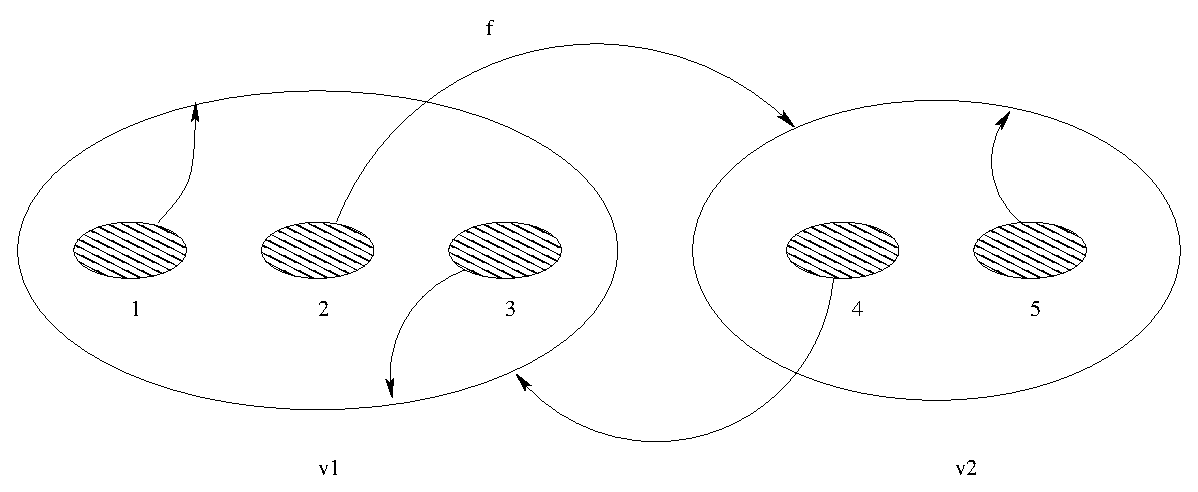
\includegraphics[scale=0.55]{cantor1.eps}
    %  note that the square brace option below is only required
    %  if you intend to produce a list of illustrations
    \caption[Shortened figure caption for the list of illustrations]
      {A Cantor repeller. Long figure captions will be indented left
      and right; short ones will be centred by default.}
    \label{cantor}
\rule[-20pt]{\textwidth}{0.6pt}
\begin{verbatim}
  \begin{figure}
    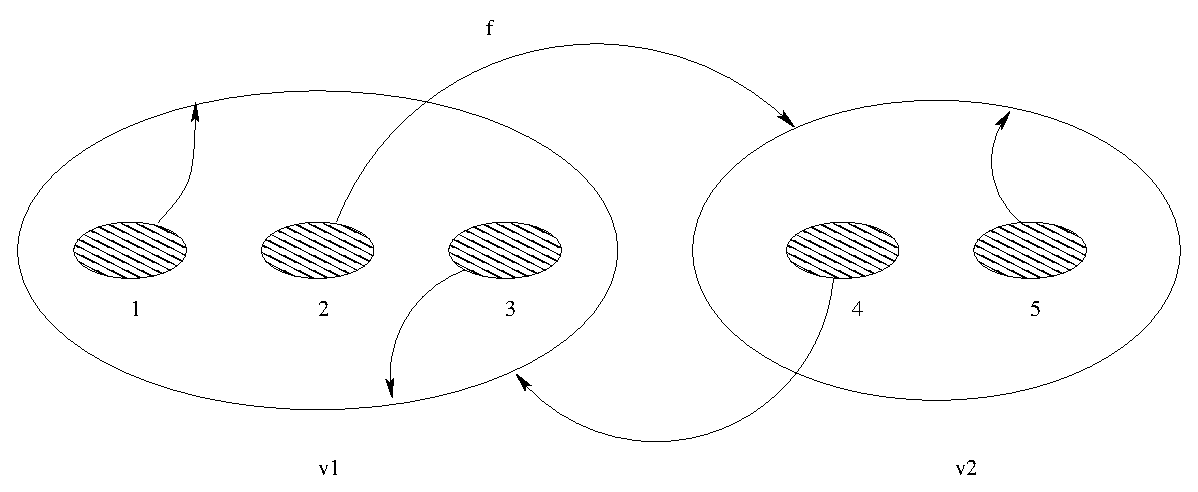
\includegraphics[scale=0.55]{cantor1.eps}
    %  note that the square brace option below is only required
    %  if you intend to produce a list of illustrations
    \caption[Shortened figure caption for the list of illustrations]
      {A Cantor repeller. Long figure captions will be indented left
      and right; short ones will be centred by default.}
    \label{cantor}
  \end{figure}
\end{verbatim}
\rule[20pt]{\textwidth}{0.5pt}
  \end{figure}

\section{Tables}

The \cambridge\ class will cope with most positioning of your tables. Table captions must be included first, the the label, then the body of the table. This is illustrated in Table~\ref{sample-table}.
  \begin{table}
    \begin{minipage}{188pt}
      %  note that the square brace option below is only required
      %  if you intend to produce a list of tables
    \caption[Shortened table caption for the list of tables]
      {Longer table captions have to be placed inside
      a minipage, otherwise they overhang the table rules.}
    \label{sample-table}
    \addtolength\tabcolsep{2pt}% to stretch columns, if required
      \begin{tabular}{@{}c@{\hspace{25pt}}ccc@{}}
        \hline \hline
        Figure\footnote{\textit{Note:} You must also use a minipage
          environment if you have footnotes.} & $hA$ & $hB$ & $hC$\\
        \hline
        1 & $\exp\left(\pi i\frac58\right)$
          & $\exp\left(\pi i\frac18\right)$ & $0$\\[3pt]
        2 & $-1$    & $\exp\left(\pi i\frac34\right)$ & $1$\\[11pt]
        3 & $-4+3i$ & $-4+3i$ & $\frac74$\\[3pt]
        4 & $-2$    & $-2$    & $\frac54 i$ \\
        \hline \hline
      \end{tabular}
    \end{minipage}
    \rule[-20pt]{\textwidth}{0.5pt}
\begin{verbatim}
  \begin{table}
    \begin{minipage}{188pt}
      %  note that the square brace option below is only required
      %  if you intend to produce a list of tables
    \caption[Shortened table caption for the list of tables]
      {Longer table captions have to be placed inside
      a minipage, otherwise they overhang the table rules.}
    \label{sample-table}
    \addtolength\tabcolsep{2pt}% to stretch columns, if required
      \begin{tabular}{@{}c@{\hspace{25pt}}ccc@{}}
        \hline \hline
        Figure\footnote{\textit{Note:} You must also use a minipage
          environment if you have footnotes.} & $hA$ & $hB$ & $hC$\\
        \hline
        1 & $\exp\left(\pi i\frac58\right)$
          & $\exp\left(\pi i\frac18\right)$ & $0$\\[3pt]
        2 & $-1$    & $\exp\left(\pi i\frac34\right)$ & $1$\\[11pt]
        3 & $-4+3i$ & $-4+3i$ & $\frac74$\\[3pt]
        4 & $-2$    & $-2$    & $\frac54 i$ \\
        \hline \hline
      \end{tabular}
    \end{minipage}
  \end{table}
\end{verbatim}
\rule[20pt]{\textwidth}{0.5pt}
  \end{table}

\subsection{My vertical rules have disappeared}

Vertical rules in tables are not \cambridge\ style, and have been automatically removed; this gives your document a truly professional look. Instead of vertical rules, we recommend the use of extra horizontal space, see Section~\ref{addhoriz}. The rules have been removed by redefining the \verb"tabular" environment. The amended definition also inserts extra vertical space above and below the horizontal rules (produced by \verb"\hline").

If you really must have them reinstated, read Section~\ref{reinstate}.

\subsection{Reinstating the vertical rules}
\label{reinstate}
Authors can revert to the standard \LaTeX\ style, if necessary. Tables will take on a rather squashed appearance, as in the \LaTeX\ book, whereby there is no added space around horizontal rules. Add the command \verb"\reinstaterules" in the preamble, and re-run your files through \LaTeX.

\subsection{There is very little space around the rules in my~table}
Tables revert to the standard, rather squashed look of standard \LaTeX\ tables for two reasons:
\begin{enumerate}
  \item you are using \verb"array.sty"; or
  \item you have chosen to reinstate vertical rules (see Section~\ref{reinstate})
\end{enumerate}
In both cases, the tabular environment is redefined.


\subsection{Adding space between columns}
\label{addhoriz}
You can add space (2pt in this example) between every column using\linebreak \verb"\addtolength\tabcolsep{2pt}". However, if you only wanted to expand the space between columns~1 and~2 to~25pt, you would do this using\linebreak  \verb"\begin{tabular}{@{}c@{\hspace{25pt}}ccc@{}}" (see Table~\ref{sample-table}).

\subsection{Adding space between rows}
If you need some form of separation between rows (for example, between rows~2 and~3 in the body of Table~\ref{sample-table}), adding \verb"[11pt]" immediately after the double backslash at the end of row~2 will add an 11pt vertical space (the equivalent of a blank line at this typesize). This is neater than adding another horizontal line.


\section{Landscape figures and tables, using rotating.sty}

Landscape figures and tables (floats) may be typeset using the \verb"rotating.sty" package. Note that the direction of rotation depends on the page number -- which requires at least two passes through \LaTeX. If we are going to know whether pages are odd or even, we need to use the \verb"\pageref" mechanism, and labels. But labels won't work unless the user has put in a caption. \textit{Beware!}

In addition to \verb"rotating.sty", you should also include \verb"floatpag.sty" and the command \verb"\rotfloatpagestyle{empty}". This combination ensures that headers and footers are removed from the float page:
\begin{verbatim}
  \usepackage{rotating}
  \usepackage{floatpag}
  \rotfloatpagestyle{empty}
\end{verbatim}
In some DVI previewers, floats may not appear rotated. If this happens, you need to convert the DVI file to PostScript or PDF.

Occasionally, when you convert a PostScript file to a PDF file, you may find that the page comes out upside-down. There will be a setting to change this. For instance, if you are using PDFCreator 0.9.7, choose the following options in this sequence:
\begin{description}
  \item Options -- Program -- PDF -- Auto-Rotate Pages: Change to `None'.
\end{description}
Other programs will have similar\vadjust{\pagebreak} procedures.


\subsection{Coding for landscape figures}

The landscape figure (Figure~\ref{sidecantor}) was typeset using the following coding:
\begin{verbatim}
  \begin{sidewaysfigure}
    \centering
    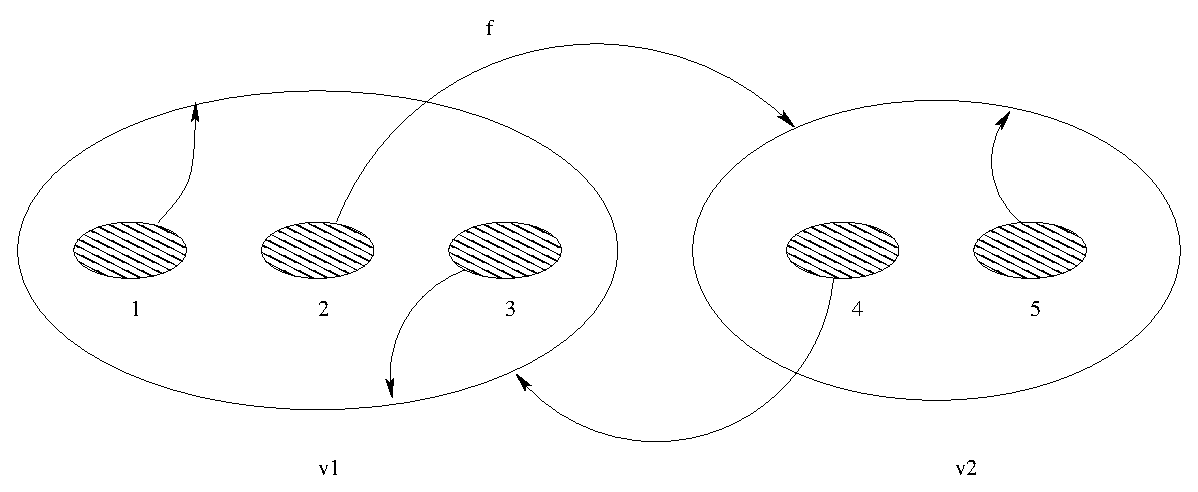
\includegraphics[scale=0.95]{cantor1.eps}
    %  note that the square brace option below is only required
    %  if you intend to produce a list of illustrations
    \caption[Landscape figure]{A Cantor repeller. Figure captions
      will be centred by default.}
    \label{sidecantor}
  \end{sidewaysfigure}
\end{verbatim}
  \begin{sidewaysfigure}
    \centering
    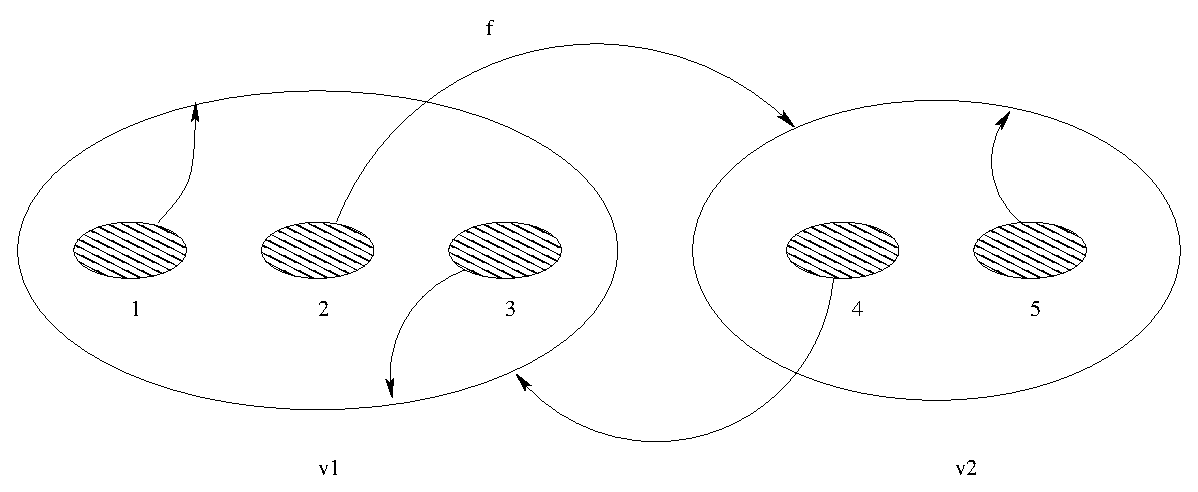
\includegraphics[scale=0.95]{cantor1.eps}
    %  note that the square brace option below is only required
    %  if you intend to produce a list of illustrations
    \caption[Landscape figure]{A Cantor repeller. Figure captions
      will be centred by default.}
    \label{sidecantor}
  \end{sidewaysfigure}



\subsection{Coding for landscape tables}

Table~\ref{sideways} has been produced using the following coding:
%
\begin{smallverbatim}
\begin{sidewaystable}
  \caption[Landscape table]{Grooved ware and beaker features, their finds and
    radiocarbon dates. For a breakdown of the pottery assemblages see
    Tables~I and~III; for the flints see Tables~II and~IV; for the animal
    bones see Table~V.}
  \label{sideways}
  \addtolength\tabcolsep{-2pt}
  \begin{tabular}{@{}lcccllccccc@{}}
  \hline\hline
  Context & Length & Breadth/  & Depth & Profile & Pottery & Flint & Animal
                                                   & Stone & Other & C14 Dates\\
  && Diameter &&&&& Bones\\[5pt]
  & m & m & m\\
  \hline\\[-5pt]
  \multicolumn{10}{@{}l}{\textbf{Grooved Ware}}\\
  784 & --   & 0.9$\phantom{0}$ &0.18  & Sloping U & P1      & $\times$46
        & $\phantom{0}$$\times$8 && $\times$2 bone & 2150 $\pm$100\,\textsc{bc}\\
  785 & --   & 1.00             &0.12   & Sloping U & P2--4  & $\times$23
                                           & $\times$21 & Hammerstone & -- & --\\
  962 & --   & 1.37             &0.20   & Sloping U & P5--6  & $\times$48
                     & $\times$57 & --& --& 1990 $\pm$80\,\textsc{bc} (Layer 4)\\
  &&&&&&&&&& 1870 $\pm$90\,\textsc{bc} (Layer 1)\\
  983 & 0.83 & 0.73             &0.25   & Stepped U & --     & $\times$18
                                & $\phantom{0}$$\times$8 & -- & Fired clay & --\\
  &&&&&&&&&&\\
  \multicolumn{10}{@{}l}{\textbf{Beaker}}\\
  552 & --   & 0.68             & 0.12  & Saucer    & P7--14 & --           & --
                                                                   & -- &-- &--\\
  790 & --   & 0.60             & 0.25  & U         & P15    & $\times$12   & --
                                                      & Quartzite-lump & -- &--\\
  794 & 2.89 & 0.75             & 0.25  & Irreg.    & P16    & $\phantom{0}$$\times$3
                                                              & -- & -- &-- &--\\
  \hline\hline
  \end{tabular}
\end{sidewaystable}
\end{smallverbatim}
%
\begin{sidewaystable}
  \caption[Landscape table]{Grooved ware and beaker features, their finds and
    radiocarbon dates. For a breakdown of the pottery assemblages see
    Tables~I and~III; for the flints see Tables~II and~IV; for the animal
    bones see Table~V.}
  \label{sideways}
  \addtolength\tabcolsep{-2pt}
  \begin{tabular}{@{}lcccllccccc@{}}
  \hline\hline
  Context & Length & Breadth/  & Depth & Profile & Pottery & Flint & Animal
                                                   & Stone & Other & C14 Dates\\
  && Diameter &&&&& Bones\\[5pt]
  & m & m & m\\
  \hline\\[-5pt]
  \multicolumn{10}{@{}l}{\textbf{Grooved Ware}}\\
  784 & --   & 0.9$\phantom{0}$ &0.18  & Sloping U & P1      & $\times$46
        & $\phantom{0}$$\times$8 && $\times$2 bone & 2150 $\pm$100\,\textsc{bc}\\
  785 & --   & 1.00             &0.12   & Sloping U & P2--4  & $\times$23
                                           & $\times$21 & Hammerstone & -- & --\\
  962 & --   & 1.37             &0.20   & Sloping U & P5--6  & $\times$48
                     & $\times$57 & --& --& 1990 $\pm$80\,\textsc{bc} (Layer 4)\\
  &&&&&&&&&& 1870 $\pm$90\,\textsc{bc} (Layer 1)\\
  983 & 0.83 & 0.73             &0.25   & Stepped U & --     & $\times$18
                                & $\phantom{0}$$\times$8 & -- & Fired clay & --\\
  &&&&&&&&&&\\
  \multicolumn{10}{@{}l}{\textbf{Beaker}}\\
  552 & --   & 0.68             & 0.12  & Saucer    & P7--14 & --           & --
                                                                   & -- &-- &--\\
  790 & --   & 0.60             & 0.25  & U         & P15    & $\times$12   & --
                                                      & Quartzite-lump & -- &--\\
  794 & 2.89 & 0.75             & 0.25  & Irreg.    & P16    & $\phantom{0}$$\times$3
                                                              & -- & -- &-- &--\\
  \hline\hline
  \end{tabular}%
\end{sidewaystable}

\endinput% features of the \cambridge\ class file
  % chap3.tex
% 2010/09/09, v2.10

\chapter{Mathematical solutions}
\label{mathsol}

\section{Why are we using amsthm.sty?}

Many authors are already using this style file, so we have decided that rather than re-invent the wheel, we will make it part of our distribution. This means that at the top of the root file must include the following lines:\\[0.5\baselineskip]
\verb"  \documentclass{"\texttt{\cambridge}\verb"}"\\
\verb"  \usepackage{amsmath}"\\
\verb"  \usepackage{amsthm}"\\[0.5\baselineskip]
As mentioned in Chapter~\ref{intro}, if your book does not use theorems, proofs, etc., then there is no need to include the amsthm package, but you do need to include these files to run this guide through \LaTeX. Note that if you are also using \verb"amsmath.sty", it \emph{must} precede \verb"amsthm.sty".

The instructions for amsthm.sty are documentated separately in \texttt{amsthdoc.pdf}. We are including \texttt{amsthm.sty} and \texttt{amsthdoc.pdf} in this distribution for your convenience, but you may find more recent versions on the web. The following sections discuss the basic features, plus a few extras.

To save time, you may cut and paste the code in Appendix~\ref{amsthmcommands} into your root file. This is a comprehensive (but not necessarily a complete) list of theorem-like environments you may wish to use.

The \verb"amsthm" commands used in this guide are detailed in Appendix~\ref{rootfile}. They are simply a subset of commands from Appendix~\ref{amsthmcommands}; some illustrate unnumbered versions.

Please note that theorems, definitions, remarks, etc.\ should be numbered in a single sequence, either by chapter (Chapter~4 would have Definition~4.1, Lemma~4.2, Lemma~4.3, Proposition~4.4, Corollary~4.5) or by section (Definition~4.1.1, Lemma~4.1.2, Lemma~4.1.3, Proposition~4.1.4, Corollary~4.1.5).

To number these elements by chapter in this guide, we have used\linebreak \verb"\newtheorem{theorem}{Theorem}[chapter]". If you prefer to have the elements numbered by section, replace \verb"[chapter]" with \verb"[section]".

\section{amsthm styles}

If no \verb"\theoremstyle" command is given, the style used will be \texttt{plain}. To specify different styles, divide your \verb"\newtheorem" commands into groups and preface each group with the appropriate \verb"\theoremstyle".

\subsection{amsthm {\upshape\texttt{plain}} style}

The \texttt{plain} style is normally used for theorems, lemmas, corollaries, propositions, conjectures, criterion and algorithms. Authors are free to define their preferred numbering systems for these. The following example resets the theorem numbers for each chapter; lemmas follow in the same sequence. We have also requested that corollaries remain unnumbered by using the starred version:
\begin{verbatim}
  \theoremstyle{plain}% default
  \newtheorem{theorem}{Theorem}[chapter]
  \newtheorem{lemma}[theorem]{Lemma}
  \newtheorem*{corollary}{Corollary}

  \begin{theorem}
    Let the scalar function\ldots
  \end{theorem}
  \begin{lemma}[Tranah]
    The first-order free surface amplitudes\ldots
  \end{lemma}
  \begin{lemma}[\citealp{MenshEst}]
    The exotic behaviours of Lagrangian\ldots
  \end{lemma}
  \begin{corollary}
    Let $G$ be the free group on\ldots
  \end{corollary}
\end{verbatim}
will produce the following output:
  \begin{theorem}
    Let the scalar function\ldots
  \end{theorem}
  \begin{lemma}[Tranah]
    The first-order free surface amplitudes\ldots
  \end{lemma}
  \begin{lemma}[\citealp{MenshEst}]
    The exotic behaviours of Lagrangian\ldots
  \end{lemma}
  \begin{corollary}
    Let $G$ be the free group on\ldots
  \end{corollary}
%
Note that Corollaries would normally be in the same numbering sequence as Theorems and Lemmas. If you'd prefer your theorems to be typeset in roman (though this is not recommended) use the amsthm \texttt{definition} style instead (see Section~\ref{amsdefn}).

\subsection{amsthm {\upshape\texttt{definition}} style}
\label{amsdefn}

The \texttt{definition} style is normally used for definitions, conditions, problems, examples. It may also be used to set up Exercises (see Appendix~\ref{amsthmcommands} for an example), although the \verb"{exerciselist}" environment described in Section~\ref{exendofsections} does the equivalent.  Again, authors are free to define their preferred numbering systems for these. However, it is most usual to continue with the same numbering sequence as for Theorems, Lemmas, etc.:
\begin{verbatim}
  \theoremstyle{definition}
  \newtheorem{definition}[theorem]{Definition}
  \newtheorem{example}[theorem]{Example}

  \begin{definition}
    The series above is the Green function\ldots
  \end{definition}
  \begin{definition}
    The correlation between the real and estimated flow\ldots
  \end{definition}
  \begin{example}
    Consider spatial and temporal problems\ldots
  \end{example}
\end{verbatim}
will produce the following output:
  \begin{definition}
    The series above is the Green function\ldots
  \end{definition}
  \begin{definition}
    The correlation between the real and estimated flow\ldots
  \end{definition}
  \begin{example}
    Consider spatial and temporal problems\ldots
  \end{example}


\subsection{amsthm {\upshape\texttt{remark}} style}
The \texttt{remark} style is normally used for remarks, notes, notation, claims, summary, acknowledgements, cases, conclusions. Again, authors are free to define their preferred numbering systems for these.
\begin{verbatim}
  \theoremstyle{remark}
  \newtheorem*{remark}{Remark}
  \newtheorem*{case}{Case}

  \begin{remark}
    The absolute amplitude of a stratified wake\ldots
  \end{remark}
  \begin{case}
    The profiles of quadratic fluctuations\ldots
  \end{case}
\end{verbatim}
will produce the following output:
  \begin{remark}
    The absolute amplitude of a stratified wake\ldots
  \end{remark}
  \begin{case}
    The profiles of quadratic fluctuations\ldots
  \end{case}

\section{Proofs}
\label{proofs}

The \verb"proof" environment is also part of the amsthm package, and provides a consistent format for proofs.
 For example,
\begin{verbatim}
  \begin{proof}
    Use $K_\lambda$ and $S_\lambda$ to translate combinators
    into $\lambda$-terms. For the converse, translate
    $\lambda x$ \ldots by [$x$] \ldots and use induction
    and the lemma.
  \end{proof}
\end{verbatim}
produces the following:
  \begin{proof}
    Use $K_\lambda$ and $S_\lambda$ to translate combinators
    into $\lambda$-terms. For the converse, translate
    $\lambda x$ \ldots by [$x$] \ldots and use induction
    and the lemma.
  \end{proof}

\subsection{Changing the word `Proof' to something else}

An optional argument allows you to substitute a different name for the standard `Proof'. To change the proof heading to read `Proof of the Pythagorean Theorem', key the following:
\begin{verbatim}
  \begin{proof}[Proof of the Pythagorean Theorem]
    Start with a generic right-angled triangle\ldots
  \end{proof}
\end{verbatim}
which produces:
  \begin{proof}[Proof of the Pythagorean Theorem]
    Start with a generic right-angled triangle\ldots
  \end{proof}


\subsection{Typesetting a proof without a \qedsymbol}

This is not part of the amsthm package. Use the \verb"proof*" version. For example,
\begin{verbatim}
  \begin{proof*}
    The apparent virtual mass coefficient\ldots
  \end{proof*}
\end{verbatim}
produces the following:
  \begin{proof*}
    The apparent virtual mass coefficient\ldots
  \end{proof*}

\subsection{Placing the \qedsymbol\ after a displayed equation}

To avoid the \qedsymbol\ dropping onto the following line at the end of a proof,
\begin{verbatim}
  \begin{proof}
    \ldots and, as we are all aware,
    \[
       E=mc^2. \qedhere
    \]
  \end{proof}
\end{verbatim}
produces the following:
  \begin{proof}
    \ldots and, as we are all aware,
    \[
       E=mc^2. \qedhere
    \]
  \end{proof}
When used with the amsmath package, version~2 or later, \verb"\qedhere" will position \qedsymbol\ flush right; with earlier versions, \qedsymbol\ will be spaced a quad away
from the end of the text or display.

If \verb"\qedhere" produces an error message in an equation, try using \verb"\mbox{\qedhere}" instead.

\subsection{Placing the \qedsymbol\ after a displayed eqnarray}

This is also not part of the amsthm package. To enable this, you need to used the starred version of \verb"proof", and add both \verb"\arrayqed" and \verb"\arrayqedhere", as shown in the following example:
\begin{verbatim}
  \begin{proof*}
    The following equations prove the theorem:
      \arrayqed
        \begin{eqnarray}
          \epsilon &=& -\frac{1}{2}U_0\frac{\mathrm{d}q'^2}
                       {\mathrm{d}x}\nonumber\\
                   &=& 10\nu\frac{q'^2}{\lambda^2}
        \arrayqedhere
        \end{eqnarray}
  \end{proof*}
\end{verbatim}
produces the following:
  \begin{proof*}
    The following equations prove the theorem:
      \arrayqed
        \begin{eqnarray}
          \epsilon &=& -\frac{1}{2}U_0\frac{\mathrm{d}q'^2}
                       {\mathrm{d}x}\nonumber\\
                   &=& 10\nu\frac{q'^2}{\lambda^2}
        \arrayqedhere
        \end{eqnarray}
  \end{proof*}

\endinput
% mathematical solutions

  \part{Closing features}
  % chap4.tex
% 2010/09/09, v2.10

\chapter{Reference and bibliography lists}

\section{Automatic lists using \textsc{Bib}\upshape{\TeX}}

We have chosen to use the natbib package because of its versatility.

First, call in \texttt{natbib.sty}. If you are using the multi-contributor option, you will get an unnumbered section heading, otherwise it will be an unnumbered chapter heading.

The bibliography file for this guide (\texttt{\cambridge guide.tex}) is called \texttt{percolation.bib}; the bibliography style is \texttt{cambridgeauthordate.bst}, so place the final two commands at the point where you would like the references to appear:
%
\begin{verbatim}
    \usepackage{natbib}
      :
  % \renewcommand{\refname}{Bibliography}
    \bibliography{percolation}
    \bibliographystyle{cambridgeauthordate}
\end{verbatim}
%
Note that if you uncomment the third line shown above, you can change the heading from `References' to `Bibliography'. Next, \LaTeX\ your book twice. Then run \textsc{Bib}\TeX\ by executing the command\\[0.5\baselineskip]
\verb"  bibtex "\texttt{\cambridge guide}\\[0.5\baselineskip]
Finally, run your book through \LaTeX\ twice again. This series of runs will generate a file called \texttt{\cambridge guide.bbl}, which will then be included by \verb"\bibliography{percolation}".

Suppose you have cited 8 entries from the `percolation' database, e.g. \verb"\citealp{MenshEst}"; \verb"\citealp{Kasymp}"; \verb"\citealp{VGFH}"; \verb"\citealp{HamMaz94}"; \verb"\citealp{HamLower}"; \verb"\citealp{AiBar87}"; \verb"\citealp{MMS}"; and \verb"\citealp{HamAtomBond}"; the output will be just those 8~entries (see page~\pageref{refs}).%
% add these entries to the list without referring to them
\nocite{MenshEst}\nocite{Kasymp}\nocite{VGFH}\nocite{HamMaz94}\nocite{HamLower}\nocite{AiBar87}\nocite{MMS}\nocite{HamAtomBond}

\section{Citations using natbib commands}
Here are some of the basic citation commands available with the natbib package; there are many more if you cannot find what you need in this list. Bear in mind that Menshikov (1985) or (Menshikov, 1985) read best, depending on context.\\*[0.5\baselineskip]
\begin{tabular}{@{}ll@{}}
\verb"\citep{MenshEst}"
    & $\rightarrow\enskip$\citep{MenshEst}\\
\verb"\citep[see][p.$\,$34]{MenshEst}"
    & $\rightarrow\enskip$\citep[see][p.$\,$34]{MenshEst}\\
\verb"\citep[e.g.][]{MenshEst}"
    & $\rightarrow\enskip$\citep[e.g.][]{MenshEst}\\
\verb"\citep[Section~2.3]{MenshEst}"
    & $\rightarrow\enskip$\citep[Section~2.3]{MenshEst}\\
\verb"\citep{MenshEst, VGFH}"\\
    & $\hspace{-70pt}\rightarrow\enskip$\citep{MenshEst, VGFH}\\
\verb"\cite{MenshEst, VGFH}"\\
    & $\hspace{-70pt}\rightarrow\enskip$\cite{MenshEst, VGFH}\\
\verb"\citealt{MenshEst}"
    & $\rightarrow\enskip$\citealt{MenshEst}\\
\verb"\cite{MenshEst}"
    & $\rightarrow\enskip$\cite{MenshEst}\\
\verb"\citealp{MenshEst}"
    & $\rightarrow\enskip$\citealp{MenshEst}\\
\verb"\citeauthor{MenshEst}"
    & $\rightarrow\enskip$\citeauthor{MenshEst}\\
\verb"\citeyearpar{MenshEst}"
    & $\rightarrow\enskip$\citeyearpar{MenshEst}\\
\verb"\citeyear{MenshEst}"
    & $\rightarrow\enskip$\citeyear{MenshEst}
\end{tabular}


\section{How to change reference entries from author--date to~numbers}
\label{numberedbiblio}

\LaTeX\ authors are used to \verb"\cite{...}" producing a reference such as~[11] in their manuscripts. If you prefer this style, it is an option within the natbib package:
\begin{verbatim}
  \usepackage[numbers]{natbib}
\end{verbatim}

\section{Keying in your reference list for an author--date system}
\label{authordatebiblio}

The entries need to be keyed as below. Note that if you uncomment the first line, you can change the heading from `References' to `Bibliography':
%
\begin{smallverbatim}
% \renewcommand{\refname}{Bibliography}
  \begin{thebibliography}{8}
    \expandafter\ifx\csname natexlab\endcsname\relax
      \def\natexlab#1{#1}\fi
    \expandafter\ifx\csname selectlanguage\endcsname\relax
      \def\selectlanguage#1{\relax}\fi

  \bibitem[Aizenman and Barsky, 1987]{AiBar87}
    Aizenman, M., and Barsky, D.~J. 1987.
    Sharpness of the phase transition in percolation models.
    {\em Comm. Math. Phys.}, {\bf 108}, 489--526.

  \bibitem[Hammersley, 1957]{HamLower}
    Hammersley, J.~M. 1957.
    Percolation processes: Lower bounds for the critical probability.
    {\em Ann. Math. Statist.}, {\bf 28}, 790--795.

  \bibitem[Hammersley, 1961]{HamAtomBond}
    Hammersley, J.~M. 1961.
    Comparison of atom and bond percolation processes.
    {\em J. Mathematical Phys.}, {\bf 2}, 728--733.

  \bibitem[Hammersley and Mazzarino, 1994]{HamMaz94}
    Hammersley, J.~M., and Mazzarino, G. 1994.
    Properties of large Eden clusters in the plane.
    {\em Combin. Probab. Comput.}, {\bf 3}, 471--505.

  \bibitem[Kesten, 1990]{Kasymp}
    Kesten, H. 1990.
    Asymptotics in high dimensions for percolation.
    Pages  219--240 of: Grimmett, G.~R., and Welsh, D.~J.~A. (eds),
    {\em Disorder in Physical Systems: A Volume in Honour of John Hammersley}.
    Oxford University Press.

  \bibitem[Menshikov, 1985]{MenshEst}
    Menshikov, M.~V. 1985.
    Estimates for percolation thresholds for lattices in {${\bf R}\sp n$}.
    {\em Dokl. Akad. Nauk SSSR}, {\bf 284}, 36--39.

  \bibitem[Menshikov et~al., 1986]{MMS}
    Menshikov, M.~V., Molchanov, S.~A., and Sidorenko, A.~F. 1986.
    Percolation theory and some applications.
    Pages  53--110 of: {\em Probability theory. Mathematical
    statistics. Theoretical cybernetics, Vol. 24 (Russian)}.
    Akad. Nauk SSSR Vsesoyuz. Inst. Nauchn. i Tekhn. Inform.
    Translated in {\em J. Soviet Math}. {\bf 42} (1988), no. 4,
    1766--1810.

  \bibitem[Vyssotsky et~al., 1961]{VGFH}
    Vyssotsky, V.~A., Gordon, S.~B., Frisch, H.~L., and Hammersley, J.~M. 1961.
    Critical percolation probabilities (bond problem).
    {\em Phys. Rev.}, {\bf 123}, 1566--1567.

  \end{thebibliography}
\end{smallverbatim}

\section{Keying in your reference list for a numbered system}

For this style, you may omit the optional square brace shown in Section~\ref{authordatebiblio}. Once again, if you uncomment the first line, you can change the heading from `References' to `Bibliography':
%
\begin{smallverbatim}
% \renewcommand{\refname}{Bibliography}
  \begin{thebibliography}{8}

  \bibitem{AiBar87}
    Aizenman, M., and Barsky, D.~J. 1987.
    Sharpness of the phase transition in percolation models.
    {\em Comm. Math. Phys.}, {\bf 108}, 489--526.

  \bibitem{HamLower}
    Hammersley, J.~M. 1957.
    Percolation processes: Lower bounds for the critical probability.
    {\em Ann. Math. Statist.}, {\bf 28}, 790--795.

  \bibitem{HamAtomBond}
    Hammersley, J.~M. 1961.
    Comparison of atom and bond percolation processes.
    {\em J. Mathematical Phys.}, {\bf 2}, 728--733.
      :
      :
  \bibitem[Vyssotsky et~al., 1961]{VGFH}
    Vyssotsky, V.~A., Gordon, S.~B., Frisch, H.~L., and Hammersley, J.~M. 1961.
    Critical percolation probabilities (bond problem).
    {\em Phys. Rev.}, {\bf 123}, 1566--1567.

  \end{thebibliography}
\end{smallverbatim}

\endinput% references and bibliographies
  % chap5.tex
% 2010/09/09, v2.10

\chapter{Indexes}
\label{indexes}

\section{Creating a single index using makeidx.sty}
To generate a single index, normally a subject index, the commands would take the form:
\begin{verbatim}
  \index{diffraction}
  \index{force!hydrodynamic}
  \index{force!interactive}
\end{verbatim}
  %\index{diffraction}%
  %\index{force!hydrodynamic}%
  %\index{force!interactive}%
The following commands are then required in the preamble:
\begin{verbatim}
  \usepackage{makeidx}
  \makeindex
\end{verbatim}
and at the point you wish your index to appear,
\begin{verbatim}
  \printindex
\end{verbatim}
Run your book through \LaTeX\ enough times so that the labels, etc., are stable. Then execute the command:\\[0.5\baselineskip]
\verb"  makeindex "\texttt{\cambridge guide}\\[0.5\baselineskip]
To include the index, you need to run \LaTeX\ one more time.


\section{Creating multiple indexes using multind.sty}
This guide has been prepared using \verb"multind.sty". This style file redefines the \verb"\makeindex", \verb"\index" and \verb"\printindex" commands to deal with multiple indexes.

Suppose you want to create an author index and a subject index. The entries should be in the text as usual, but take the following form:
\begin{verbatim}
  \index{authors}{Young, P.D.F.}
  \index{authors}{Tranah, D.A.}
  \index{authors}{Peterson, K.}
  \index{subject}{diffraction}
  \index{subject}{force!hydrodynamic}
  \index{subject}{force!interactive}
\end{verbatim}
  \index{authors}{Young, P.D.F.}%
  \index{authors}{Tranah, D.A.}%
  \index{authors}{Peterson, K.}%
  \index{subject}{diffraction}%
  \index{subject}{force!hydrodynamic}%
  \index{subject}{force!interactive}%
In the preamble, you need to add the following lines:
\begin{verbatim}
  \usepackage{multind}\ProvidesPackage{multind}
  \makeindex{authors}
  \makeindex{subject}
\end{verbatim}
It is crucial to add the command \verb"\ProvidesPackage{multind}"; this will send a message to the class file to re-style the index into the \cambridge\ style. You will get a warning in your log file:
\begin{verbatim}
  LaTeX Warning: You have requested package `',
                 but the package provides `multind'.
\end{verbatim}
which can be ignored. At the point where you wish your indexes to appear, you then need the commands:
\begin{verbatim}
  \printindex{authors}{Author index}
  \printindex{subject}{Subject index}
\end{verbatim}
Run your book through \LaTeX\ enough times so that the labels, etc., are stable. Then execute the commands:
\begin{verbatim}
  makeindex authors
  makeindex subject
\end{verbatim}
To include the indexes, you need to run \LaTeX\ one more time.

\section{Creating multiple indexes using index.sty}

This style file allows you to define new indexes. Suppose you want to create an author index as well as a normal subject index. The entries should be in the text as usual, but take the following form:
\begin{verbatim}
  \index[aut]{Young, P.D.F.}
  \index[aut]{Tranah, D.A.}
  \index[aut]{Peterson, K.}
  \index{diffraction}
  \index{force!hydrodynamic}
  \index{force!interactive}
\end{verbatim}
  %\index[aut]{Young, P.D.F.}%
  %\index[aut]{Tranah, D.A.}%
  %\index[aut]{Peterson, K.}
  %\index{diffraction}%
  %\index{force!hydrodynamic}%
  %\index{force!interactive}%
To create the extra author index, you need to have the following lines in the preamble:
\begin{verbatim}
  \usepackage{index}
  \makeindex
  \newindex{aut}{adx}{and}{Author index}
\end{verbatim}
At the point where you wish your indexes to appear, use:
\begin{verbatim}
  \printindex[aut]
  \printindex
\end{verbatim}
Run your book through \LaTeX\ enough times so that the labels, etc., are stable. Then execute the commands:\\[0.5\baselineskip]
\verb"  makeindex -o "\texttt{\cambridge guide.and \cambridge guide.adx}\\
\verb"  makeindex "\texttt{\cambridge guide}\\[0.5\baselineskip]
To include the indexes, you need to run \LaTeX\ one more time.

\subsection{Caution -- from the authors of index.sty}

In order to implement \verb"index.sty", it's been necessary to modify a number of \LaTeX\ commands seemingly unrelated to indexing, namely, \verb"\@starttoc", \verb"\raggedbottom", \verb"\flushbottom", \verb"\addcontents", \verb"\markboth", and \verb"\markright". Naturally, this could cause incompatibilities between \texttt{index.sty} and any style files that either redefine these same commands or make specific assumptions about how they operate.

The redefinition of \verb"\@starttoc" is particularly bad, since it introduces an incompatibility with the AMS document classes. This will be addressed soon.

In the current implementation, \texttt{index.sty} uses one output stream for each index.  Since there are a limited number of output indexes, this means that there is a limit on the number of indexes you can have in a document.  There is more information on this in \verb"index.dtx" which is part of the \verb"index.sty" distribution.\\[\baselineskip]
%
\textit{For these reasons, whilst all care has been taken to deal with these changes in \cambridge.cls, if you do find incompatibilities with other files, please contact us at texline@cambridge.org with your source files, class and style files, and log file.}

\endinput
% single and multiple indexes

  \backmatter
% if you only have one appendix, use \oneappendix instead of \appendix
  \appendix
  % appendixA.tex
% 2010/09/09, v2.10

\chapter{Typesetting appendices}

\section{Single-contributor books}
\subsection{How to typeset one appendix}
If you have just one appendix, say \verb"appendix.tex", you will want to generate a chapter head `Appendix' rather than `Appendix A'. Use \verb"\oneappendix" in the main file, as follows:
\begin{verbatim}
  \oneappendix
  % \iffalse meta-comment
% apendix.dtx
% Author: Peter Wilson, Herries Press
% Maintainer: Will Robertson (will dot robertson at latex-project dot org)
% Copyright 1998--2004 Peter R. Wilson
%
% This work may be distributed and/or modified under the
% conditions of the LaTeX Project Public License, either
% version 1.3c of this license or (at your option) any 
% later version: <http://www.latex-project.org/lppl.txt>
%
% This work has the LPPL maintenance status "maintained".
% The Current Maintainer of this work is Will Robertson.
%
% This work consists of the files listed in the README file.
%
% 
%<*driver>
\documentclass{ltxdoc}
\EnableCrossrefs
\CodelineIndex
\setcounter{StandardModuleDepth}{1}
\begin{document}
  \DocInput{appendix.dtx}
\end{document}
%</driver>
%
% \fi
%
% \CheckSum{481}
%
% \DoNotIndex{\',\.,\@M,\@@input,\@addtoreset,\@arabic,\@badmath}
% \DoNotIndex{\@centercr,\@cite}
% \DoNotIndex{\@dotsep,\@empty,\@float,\@gobble,\@gobbletwo,\@ignoretrue}
% \DoNotIndex{\@input,\@ixpt,\@m}
% \DoNotIndex{\@minus,\@mkboth,\@ne,\@nil,\@nomath,\@plus,\@set@topoint}
% \DoNotIndex{\@tempboxa,\@tempcnta,\@tempdima,\@tempdimb}
% \DoNotIndex{\@tempswafalse,\@tempswatrue,\@viipt,\@viiipt,\@vipt}
% \DoNotIndex{\@vpt,\@warning,\@xiipt,\@xipt,\@xivpt,\@xpt,\@xviipt}
% \DoNotIndex{\@xxpt,\@xxvpt,\\,\ ,\addpenalty,\addtolength,\addvspace}
% \DoNotIndex{\advance,\Alph,\alph}
% \DoNotIndex{\arabic,\ast,\begin,\begingroup,\bfseries,\bgroup,\box}
% \DoNotIndex{\bullet}
% \DoNotIndex{\cdot,\cite,\CodelineIndex,\cr,\day,\DeclareOption}
% \DoNotIndex{\def,\DisableCrossrefs,\divide,\DocInput,\documentclass}
% \DoNotIndex{\DoNotIndex,\egroup,\ifdim,\else,\fi,\em,\endtrivlist}
% \DoNotIndex{\EnableCrossrefs,\end,\end@dblfloat,\end@float,\endgroup}
% \DoNotIndex{\endlist,\everycr,\everypar,\ExecuteOptions,\expandafter}
% \DoNotIndex{\fbox}
% \DoNotIndex{\filedate,\filename,\fileversion,\fontsize,\framebox,\gdef}
% \DoNotIndex{\global,\halign,\hangindent,\hbox,\hfil,\hfill,\hrule}
% \DoNotIndex{\hsize,\hskip,\hspace,\hss,\if@tempswa,\ifcase,\or,\fi,\fi}
% \DoNotIndex{\ifhmode,\ifvmode,\ifnum,\iftrue,\ifx,\fi,\fi,\fi,\fi,\fi}
% \DoNotIndex{\input}
% \DoNotIndex{\jobname,\kern,\leavevmode,\let,\leftmark}
% \DoNotIndex{\list,\llap,\long,\m@ne,\m@th,\mark,\markboth,\markright}
% \DoNotIndex{\month,\newcommand,\newcounter,\newenvironment}
% \DoNotIndex{\NeedsTeXFormat,\newdimen}
% \DoNotIndex{\newlength,\newpage,\nobreak,\noindent,\null,\number}
% \DoNotIndex{\numberline,\OldMakeindex,\OnlyDescription,\p@}
% \DoNotIndex{\pagestyle,\par,\paragraph,\paragraphmark,\parfillskip}
% \DoNotIndex{\penalty,\PrintChanges,\PrintIndex,\ProcessOptions}
% \DoNotIndex{\protect,\ProvidesClass,\raggedbottom,\raggedright}
% \DoNotIndex{\refstepcounter,\relax,\renewcommand,\reset@font}
% \DoNotIndex{\rightmargin,\rightmark,\rightskip,\rlap,\rmfamily,\roman}
% \DoNotIndex{\roman,\secdef,\selectfont,\setbox,\setcounter,\setlength}
% \DoNotIndex{\settowidth,\sfcode,\skip,\sloppy,\slshape,\space}
% \DoNotIndex{\symbol,\the,\trivlist,\typeout,\tw@,\undefined,\uppercase}
% \DoNotIndex{\usecounter,\usefont,\usepackage,\vfil,\vfill,\viiipt}
% \DoNotIndex{\viipt,\vipt,\vskip,\vspace}
% \DoNotIndex{\wd,\xiipt,\year,\z@}
%
% \changes{v1.0}{1998/11/29}{First public release}
% \changes{v1.0a}{1999/07/28}{Added text about includes}
% \changes{v1.1}{2000/02/29}{Extended appendices}
% \changes{v1.1}{2000/02/29}{Added subappendices}
% \changes{v1.1a}{2001/03/15}{Fixed problem with \cs{addappheadtotoc}}
% \changes{v1.2}{2002/08/06}{Compatibility with hyperref bookmarks}
% \changes{v1.2}{2002/08/06}{Don't need the ifthen package any more}
% \changes{v1.2a}{2004/04/16}{Changed license and contact details}
% \changes{v1.2b}{2009/09/02}{New maintainer (Will Robertson)}
%
% \def\dtxfile{appendix.dtx}
% \def\fileversion{v1.1}  \def\filedate{2000/02/29}
% \def\fileversion{v1.1a} \def\filedate{2001/03/15}
% \def\fileversion{v1.2}  \def\filedate{2002/08/06}
% \def\fileversion{v1.2a} \def\filedate{2004/04/16}
% \def\fileversion{v1.2b} \def\filedate{2009/09/02}
%
% \newcommand*{\Lpack}[1]{\textsf {#1}}           ^^A typeset a package
% \newcommand*{\Lopt}[1]{\textsf {#1}}            ^^A typeset an option
% \newcommand*{\file}[1]{\texttt {#1}}            ^^A typeset a file
% \newcommand*{\Lcount}[1]{\textsl {\small#1}}    ^^A typeset a counter
% \newcommand*{\pstyle}[1]{\textsl {#1}}          ^^A typeset a pagestyle
% \newcommand*{\Lenv}[1]{\texttt {#1}}            ^^A typeset an environment
%
% \title{The \Lpack{appendix} package\thanks{This
%        file (\texttt{\dtxfile}) has version number \fileversion, last revised
%        \filedate.}}
%
% \author{
%   Author: Peter Wilson, Herries Press\\
%   Maintainer: Will Robertson\\
%   \texttt{will dot robertson at latex-project dot org}
% }
% \date{\filedate}
% \maketitle
% \begin{abstract}
%    The \Lpack{appendix} package provides some facilities for modifying the
% typesetting of appendix titles. Further, |(sub)appendices| environments
% are available that can be used, for example, for per chapter/section
% appendices.
%
% The package
% is designed to work only with classes that have a |\chapter| and/or
% |\section| command. It has not been tested with other packages
% that change the definitions of the sectioning commands. 
% \end{abstract}
% \tableofcontents
%
%
%
%
% \section{Introduction}
%
% In the standard classes the |\appendix| command does the following:
% \begin{itemize}
% \item For classes with Chapters:
%    \begin{itemize}
%    \item Resets the chapter and section counters to zero
%    \item Sets |\@chapapp| to |\appendixname|.
%    \item Redefines |\thechapter| to produce alphabetic appendix numbers.
%    \end{itemize}
% \item For the other classes
%    \begin{itemize}
%    \item Resets the section and subsection counters to zero.
%    \item Redefines |\thesection| to produce alphabetic appendix numbers.
%    \end{itemize}
%  \end{itemize}
%
% The \Lpack{appendix} package provides additional appendixing capabilities.
% It cooperates with the \Lpack{hyperref} 
% package\footnote{With thanks to Hylke W. van Dijk 
% (\texttt{hylke@ubicom.tudelft.nl}) who pointed out that version~1.1 did 
% not and set me on the track for supporting the \Lpack{hyperref} package.}
% but may be problematic when used with packages that change the definition
% of the sectioning commands.
%
% Portions of the package were developed as part of a class
% and package bundle for typesetting ISO standards~\cite{PRW96i}.
% This manual is typeset according to the conventions of the
% \LaTeX{} \textsc{docstrip} utility which enables the automatic
% extraction of the \LaTeX{} macro source files~\cite{GOOSSENS94}.
%
%    Section~\ref{sec:usc} describes the usage of the package.
% Commented source code for the package is in Section~\ref{sec:code}.
%
% \section{The \Lpack{appendix} package} \label{sec:usc}
%
% The \Lpack{appendix} package provides some commands that can be
% used in addition to the |\appendix| command. It also provides
% a new environment that can be used instead of the |\appendix| command.
% The environment provides some addtional actions with respect to
% the simple |\appendix|. First the new commands will be described and
% then the new environment will be discussed.
%
% \DescribeMacro{\appendixpage}
%  The |\appendixpage| command will typeset a heading in the style of
% a |\part| heading for the class. The wording of the heading is
% given by the value of |\appendixpagename|.
%
% \DescribeMacro{\addappheadtotoc}
% This command will insert general heading into the Table of Contents (ToC).
% The text is given by the value of |\appendixtocname|. If used, the command
% must come before the first appendix, as it is meant to be used to introduce
% the appendix titles in the ToC.
%
% \changes{v1.1a}{2001/03/15}{Added NOTE about \cs{addappheadtotoc} page number}
% The above commands can be used in conjunction with the traditional
% |\appendix| command, which they should immediately follow. For example:
% \begin{verbatim}
% \appendix
% \appendixpage
% \addappheadtotoc
% \end{verbatim}
%
% \DescribeMacro{\noappendicestocpagenum}
% \DescribeMacro{\appendicestocpagenum}
% By default the |\addappheadtotoc| command puts a page number
% in the ToC. This can be prevented by using |\noappendicestocpagenum|.
% For symmetry, the |\appendicestocpagenum| command ensures that
% a page number is put in the ToC.
%
% \textbf{NOTE:} Unless |\noappendicestocpagenum| is used 
% the |\addappheadtotoc| command uses the 
% current page number
% when it makes the entry in the ToC. The |\appendixpage| command puts
% a heading in the document like a |\part| heading; in un-chaptered documents
% the |\part| heading appears in the ordinary run of the text like a 
% |\section| heading, but in chaptered documents it is on a page by itself.
% That is, in chaptered documents |\appendixpage| does a |\clear[double]page|
% typesets the heading, and then does another |\clear[double]page|. Therefore,
% in a chaptered document the above sequence of 
% commands will use the page number
% \emph{after} the |\appendixpage| as the ToC 
% entry\footnote{With thanks to Eduardo Jacob (\texttt{edu@kender.es})
% for pointing this out.} and if the ordering
% is reversed (i.e., |\addappheadtotoc| |\appendixname|) then the page number
% \emph{before} |\appendixname| will be used as the ToC entry. For chaptered
% documents it is probably best to do: \\
% |    \clearpage % or \cleardoublepage| \\
% |    \addappheadtotoc| \\
% |    \appendixpage| \\
% which will use the page number of |\appendixpage| as the ToC entry.
% 
%
% \DescribeMacro{\appendixname}
% \DescribeMacro{\appendixtocname}
% \DescribeMacro{\appendixpagename}
% The |\appendixname| command is defined in those classes that provide
% for chapters. It is provided in this package whether or not it has
% been defined in the class. It's default value is `Appendix'.
% The default value of both |\appendixtocname| and |\appendixpagename| is 
% `Appendices'. These names can all be changed via |\renewcommand|.
% For example,
% \begin{verbatim}
% \renewcommand{\appendixtocname}{List of appendices}
% \end{verbatim}
%
% \DescribeEnv{appendices}
% The |appendices| environment can be used instead of the |\appendix|
% command. It provides more functionality than is possible from the 
% combination of the |\appendix|, |\addappheadtotoc| and |\appendixpage|
% commands.
% The functions of the |appendices| environment are usually accessed through
% the package options, but there are declarations that mey be used insted. 
% The options are:
% \begin{itemize}
% \item \Lopt{toc} Put a header (e.g., `Appendices') into the Table
%       of Contents (the ToC) before listing the appendices. (This
%       is done by calling the |\addappheadtotoc| command.)
% \item \Lopt{page} Puts a title (e.g., `Appendices') into the document
%       at the point where the |appendices| environment is begun.
%       (This is done by calling the |\appendixpage| command.)
% \item \Lopt{title} Adds a name (e.g., `Appendix') before each appendix
%       title in the body of the document. 
%       The name is given by the value of |\appendixname|.
%       Note that this is the default behaviour for classes that have
%       chapters.
% \item \Lopt{titletoc} Adds a name (e.g., `Appendix') before each
%        appendix listed in the ToC.
%       The name is given by the value of |\appendixname|.
% \item \Lopt{header} Adds a name (e.g., `Appendix') before each appendix
%        in page headers.
%       The name is given by the value of |\appendixname|.
%       Note that this is the default behaviour for classes that have
%       chapters.
% \end{itemize}
%
%    Depending on the particular package options that are set and the
% document class, the
% |appendices| environment may change the definition of elements of
% the sectioning commands (e.g., |\chapter| or |\section|).
% This may be a problem if the environment
% is used in conjunction with any other package that makes changes to
% these commands. If this is the case, then you will have to examine the
% code for the |appendices| environment and make any necessary changes
% to one or the other of the packages (via your own package file).
% The changes to the sectional heading commands are discarded at the
% end of the |appendices| environment.
%
% \DescribeMacro{\appendixtocon}
% \DescribeMacro{\appendixtocoff}
% |\appendixtocon| is a declaration equivalent to the \Lopt{toc} option.
% The |\appendixtocoff| declaration is equivalent to not using that option.
%
% \DescribeMacro{\appendixpageon}
% \DescribeMacro{\appendixpageoff}
% |\appendixpagecon| is a declaration equivalent to the \Lopt{page} option.
% The |\appendixpageoff| declaration is equivalent to not using 
% that option.
%
% \DescribeMacro{\appendixtitleon}
% \DescribeMacro{\appendixtitleoff}
% |\appendixtitleon| is a declaration equivalent to the \Lopt{title} option.
% The |\appendixtitleoff| declaration is equivalent to not using 
% that option.
%
% \DescribeMacro{\appendixtitletocon}
% \DescribeMacro{\appendixtitletocoff}
% |\appendixtitletocon| is a declaration equivalent to the \Lopt{titletoc} option.
% The |\appendixtitletocoff| declaration is equivalent to not using 
% that option.
%
% \DescribeMacro{\appendixheaderon}
% \DescribeMacro{\appendixheaderoff}
% |\appendixheaderon| is a declaration equivalent to the \Lopt{header} option.
% The |\appendixheaderoff| declaration is equivalent to not using 
% that option.
%
% \DescribeMacro{\restoreapp}
%     The |appendices| environment restores the prior value of the 
% chapter/section counter at the end of the environment, so the
% environment may be used between the main document divisions. By default,
% the appendix counter value is saved and restored by the environment. That
% means that appendices in a series of |appendices| environments will
% be lettered sequentially. To make the lettering start from A each time,
% put the following into the preamble: \\
% |\renewcommand{\restoreapp}{}|
%
% \DescribeEnv{subappendices}
% Within the |subappendices| environment, an appendix is introduced by a
% |\section| command in chaptered documents, otherwise it is introduced
% by a |\subsection| command. Effectively, this provides for appendices 
% at the end of a main document division, as an integral
% part of the division. The |subappendices| environment supports only
% the \Lopt{title} and \Lopt{titletoc} options.
%
% \DescribeMacro{\setthesection}
% \DescribeMacro{\setthesubsection}
% By default, the `subappendices' are numbered like normal (sub)sections,
% except that the (sub)section number itself is typeset as an uppercase
% letter. This behaviour can be changed by redefining these |\setthe...|
% commands. For example, to just have a letter not prepended by the main
% division number, do: \\
% |\renewcommand{\setthesection}{\Alph{section}}| or \\
% |\renewcommand{\setthesubsection}{\Alph{subsection}}| as appropriate.
%
% \subsection{Known problems}
%
%    There is an unfortunate interaction between the \LaTeX{} kernel commands
% |\include| and |\addcontentsline|. If these are used like this:
% \begin{verbatim}
% \addcontentsline{toc}{...}{addtotoc}
% \include{import}
% \end{verbatim}
% then the text of the |\addcontentsline| command (`addtotoc' in the example)
% is not written to the
% appropriate (toc) file until \textit{after} the included file has written all
% its entries out to the (toc) file. As far as I can tell, there is no way 
% around this behaviour without rewriting parts of the \LaTeX{} kernel code.
% 
%     It is thus up to the author to avoid putting an |\addcontentsline| command
% (or a command that internally uses |\addcontentsline|, as does the
% |\addappheadtotoc| command) before
% an |\include|d file that writes out to the same file. Things work as
% expected if the |\addcontentsline| command is placed within the |\include|d
% file, or if the imported file is |\input|ed instead of |\include|d.
%
% \StopEventually{}
%
% \section{The package code} \label{sec:code}
%
%    Announce the name and version of the package, which requires
% \LaTeXe.
%    \begin{macrocode}
%<*usc>
\NeedsTeXFormat{LaTeX2e}
\ProvidesPackage{appendix}[2009/09/02 v1.2b extra appendix facilities]

%    \end{macrocode}
%
% In order to try and avoid name clashes with other packages, each internal
% name will include the character string |@pp|.
%
%
% \begin{macro}{\if@knownclass@pp}
% \begin{macro}{\if@chapter@pp}
%    These are used when we need to decide what appendix style is being used
%    for the document. Assume the \Lpack{article} class or other without
% chapters.
% \changes{v1.1a}{2001/03/15}{Checking on sectional commands, not classes}
%    \begin{macrocode}
\newif\if@chapter@pp\@chapter@ppfalse
\newif\if@knownclass@pp\@knownclass@ppfalse
%    \end{macrocode}
%    Check the sectioning commands.
%    \begin{macrocode}
\@ifundefined{chapter}{%
  \@ifundefined{section}{}{\@knownclass@pptrue}}{%
  \@chapter@pptrue\@knownclass@pptrue}
%    \end{macrocode}
% \end{macro}
% \end{macro}
%
% \begin{macro}{\phantomsection}
% \begin{macro}{\the@pps}
% \begin{macro}{\if@pphyper}
% We need to provide |\phantomsection| if \Lpack{hyperref} is not
% used and, whether or not \Lpack{hyperref} is used, we need to define
% a counter here to support potential hyperrefs (used to disambiguate
% (sub)appendices).
% |\if@pphyper| is TRUE if the \Lpack{hyperref} package is used.
% \changes{v1.2}{2002/08/06}{Added the \texttt{@pps} counter}
% \changes{v1.2}{2002/08/06}{Added \cs{if@pphyper}}
%    \begin{macrocode}
\providecommand{\phantomsection}{}
\newcounter{@pps}
  \renewcommand{\the@pps}{\alph{@pps}}
\newif\if@pphyper
  \@pphyperfalse
\AtBeginDocument{%
  \@ifpackageloaded{hyperref}{\@pphypertrue}{}}

%    \end{macrocode}
% \end{macro}
% \end{macro}
% \end{macro}
%
% \begin{macro}{\if@dotoc@pp}
% \begin{macro}{\if@dotitle@pp}
% \begin{macro}{\if@dotitletoc@pp}
% \begin{macro}{\if@dohead@pp}
% \begin{macro}{\if@dopage@pp}
%    A set of booleans for the options. Default is the |appendices|
% environment does nothing more than the |\appendix| command does
% unless one or more options are set.
%    \begin{macrocode}
\newif\if@dotoc@pp\@dotoc@ppfalse
\newif\if@dotitle@pp\@dotitle@ppfalse
\newif\if@dotitletoc@pp\@dotitletoc@ppfalse
\newif\if@dohead@pp\@dohead@ppfalse
\newif\if@dopage@pp\@dopage@ppfalse
%    \end{macrocode}
% \end{macro}
% \end{macro}
% \end{macro}
% \end{macro}
% \end{macro}
%
%    Now we can do the five options.
%    \begin{macrocode}
\DeclareOption{toc}{\@dotoc@pptrue}
\DeclareOption{title}{\@dotitle@pptrue}
\DeclareOption{titletoc}{\@dotitletoc@pptrue}
\DeclareOption{header}{\@dohead@pptrue}
\DeclareOption{page}{\@dopage@pptrue}
%    \end{macrocode}
% Process the options now.
%    \begin{macrocode}
\ProcessOptions\relax
%    \end{macrocode}
%
% Issue a warning if |\chapter| and |\section| are undefined, then
% quit.
%    \begin{macrocode}
\newcommand{\@ppendinput}{}
\if@knownclass@pp\else
  \PackageWarningNoLine{appendix}%
    {There is no \protect\chapter\space or \protect\section\space command.\MessageBreak
     The appendix package will not be used}
  \renewcommand{\@ppendinput}{\endinput}
\fi
\@ppendinput

%    \end{macrocode}
%
% \begin{macro}{\appendixtocon}
% \begin{macro}{\appendixtocoff}
% Declarative forms of the \Lopt{toc} option.
% \changes{v1.2}{2002/08/06}{Added declarations for the options}
%    \begin{macrocode}
\newcommand{\appendixtocon}{\@dotoc@pptrue}
\newcommand{\appendixtocoff}{\@dotoc@ppfalse}
%    \end{macrocode}
% \end{macro}
% \end{macro}
%
% \begin{macro}{\appendixpageon}
% \begin{macro}{\appendixpageoff}
% Declarative forms of the \Lopt{page} option.
%    \begin{macrocode}
\newcommand{\appendixpageon}{\@dopage@pptrue}
\newcommand{\appendixpageoff}{\@dopage@ppfalse}
%    \end{macrocode}
% \end{macro}
% \end{macro}
%
% \begin{macro}{\appendixtitleon}
% \begin{macro}{\appendixtitleoff}
% Declarative forms of the \Lopt{title} option.
%    \begin{macrocode}
\newcommand{\appendixtitleon}{\@dotitle@pptrue}
\newcommand{\appendixtitleoff}{\@dotitle@ppfalse}
%    \end{macrocode}
% \end{macro}
% \end{macro}
%
% \begin{macro}{\appendixtitletocon}
% \begin{macro}{\appendixtitletocoff}
% Declarative forms of the \Lopt{titletoc} option.
%    \begin{macrocode}
\newcommand{\appendixtitletocon}{\@dotitletoc@pptrue}
\newcommand{\appendixtitletocoff}{\@dotitletoc@ppfalse}
%    \end{macrocode}
% \end{macro}
% \end{macro}
%
% \begin{macro}{\appendixheaderon}
% \begin{macro}{\appendixheaderoff}
% Declarative forms of the \Lopt{header} option.
%    \begin{macrocode}
\newcommand{\appendixheaderon}{\@dohead@pptrue}
\newcommand{\appendixheaderoff}{\@dohead@ppfalse}
%    \end{macrocode}
% \end{macro}
% \end{macro}
%
% \begin{macro}{\@ppsavesec}
% \begin{macro}{\@pprestoresec}
% \begin{macro}{\@ppsaveapp}
% \begin{macro}{\restoreapp}
%  For the |appendices| environment we need to save and restore the
% main document division number and the appendix number. The |\restoreapp|
% command is the one for the user.
% \changes{v1.1}{2000/02/29}{Added commands to save and restore sectional numbering}
%    \begin{macrocode}
\newcounter{@ppsavesec}
\newcounter{@ppsaveapp}
\setcounter{@ppsaveapp}{0}
\newcommand{\@ppsavesec}{%
  \if@chapter@pp \setcounter{@ppsavesec}{\value{chapter}} \else
                 \setcounter{@ppsavesec}{\value{section}} \fi}
\newcommand{\@pprestoresec}{%
  \if@chapter@pp \setcounter{chapter}{\value{@ppsavesec}} \else
                 \setcounter{section}{\value{@ppsavesec}} \fi}
\newcommand{\@ppsaveapp}{%
  \if@chapter@pp \setcounter{@ppsaveapp}{\value{chapter}} \else
                 \setcounter{@ppsaveapp}{\value{section}} \fi}
\newcommand{\restoreapp}{%
  \if@chapter@pp \setcounter{chapter}{\value{@ppsaveapp}} \else
                 \setcounter{section}{\value{@ppsaveapp}} \fi}
%    \end{macrocode}
% \end{macro}
% \end{macro}
% \end{macro}
% \end{macro}
%
% \begin{macro}{\appendixname}
% \begin{macro}{\appendixtocname}
% \begin{macro}{\appendixpagename}
%  These commands hold the names that might be used. |\appendixname|
% may have been defined in the class. The others are new.
%    \begin{macrocode}
\providecommand{\appendixname}{Appendix}
\newcommand{\appendixtocname}{Appendices}
\newcommand{\appendixpagename}{Appendices}
%    \end{macrocode}
% \end{macro}
% \end{macro}
% \end{macro}
%
% \begin{macro}{\appendixpage}
% The command to typeset a page announcing the start of the appendices.
% It is based on the |\part| definition (either from the \Lpack{book}
% class or the \Lpack{article} class). 
%    \begin{macrocode}
\newcommand{\appendixpage}{%
  \if@chapter@pp \@chap@pppage \else \@sec@pppage \fi
}
%    \end{macrocode}
% \end{macro}
%
% \begin{macro}{\clear@ppage}
%  The non-chaptered classes do not define |\if@openright|, but we need to 
% use this for chaptered documents to clear the appropriate pages.
% |\clear@ppage| does the right thing, but must only be called in
% chapter related code, otherwise there will be error message like 
% |extra \else| or |extra \fi|.
%    \begin{macrocode}
\newcommand{\clear@ppage}{%
  \if@openright\cleardoublepage\else\clearpage\fi}

%    \end{macrocode}
% \end{macro}
%
% \begin{macro}{\@chap@pppage}
% Do an appendix page in chapter style.
% Copy code from the \Lpack{book} class |\part| command, but use 
% |\appendixpagename| as the title.
%    \begin{macrocode}
\newcommand{\@chap@pppage}{%
  \clear@ppage
  \thispagestyle{plain}%
  \if@twocolumn\onecolumn\@tempswatrue\else\@tempswafalse\fi
  \null\vfil
  \markboth{}{}%
  {\centering
   \interlinepenalty \@M
   \normalfont
   \Huge \bfseries \appendixpagename\par}%
%    \end{macrocode}
% Add to ToC if requested
%    \begin{macrocode}
  \if@dotoc@pp
    \addappheadtotoc
  \fi
%    \end{macrocode}
% In the \Lpack{book} class the |\part| command is finished off by calling
% |\@endpart|. There are two problems with this in this package. (1)
% |\@endpart| is not defined in \Lpack{article} style classes and (2)
% it always throws a blank page which does not look good if the \Lopt{openany}
% option is used. So, code it all up here.
%    \begin{macrocode}
  \vfil\newpage
  \if@twoside
    \if@openright
      \null
      \thispagestyle{empty}%
      \newpage
    \fi
  \fi
  \if@tempswa
    \twocolumn
  \fi
}

%    \end{macrocode}
% \end{macro}
%
% \begin{macro}{\@sec@pppage}
% Copy code from the \Lpack{article} class |\part| command, but use 
% |\appendixpagename| as 
% the title.
%    \begin{macrocode}
\newcommand{\@sec@pppage}{%
  \par
  \addvspace{4ex}%
  \@afterindentfalse
  {\parindent \z@ \raggedright
   \interlinepenalty \@M
   \normalfont
   \huge \bfseries \appendixpagename%
   \markboth{}{}\par}%
%    \end{macrocode}
% Add to ToC if requested
%    \begin{macrocode}
  \if@dotoc@pp
    \addappheadtotoc
  \fi
  \nobreak
  \vskip 3ex
  \@afterheading
}

%    \end{macrocode}
% \end{macro}
%
% \begin{macro}{\if@pptocpage}
% \begin{macro}{\noappendicestocpagenum}
% \begin{macro}{\appendicestocpagenum}
% \begin{macro}{\addappheadtotoc}
% The |\addappheadtotoc| command adds an `appendices' line to the ToC. 
% The style is the same
% as used in \Lpack{tocbibind} for the `List of figures' line. That is,
% as a Chapter heading or a Section heading. |\if@pptocpage| controls
% whether ot not a page number is put into the ToC.
% \changes{v1.2}{2002/08/06}{Added \cs{noappendicestocpagenum} and changed
%                           \cs{addappheadtotoc}}
%    \begin{macrocode}
\newif\if@pptocpage
  \@pptocpagetrue
\newcommand{\noappendicestocpagenum}{\@pptocpagefalse}
\newcommand{\appendicestocpagenum}{\@pptocpagetrue}
\newcommand{\addappheadtotoc}{%
  \phantomsection
  \if@chapter@pp
%    \end{macrocode}
% Chaptered document
%    \begin{macrocode}
    \if@pptocpage
      \addcontentsline{toc}{chapter}{\appendixtocname}%
    \else
      \if@pphyper
        \addtocontents{toc}%
          {\protect\contentsline{chapter}{\appendixtocname}{}{\@currentHref}}%
      \else
        \addtocontents{toc}%
          {\protect\contentsline{chapter}{\appendixtocname}{}}%
      \fi
    \fi      
  \else
%    \end{macrocode}
% Not a chaptered document
%    \begin{macrocode}
    \if@pptocpage
      \addcontentsline{toc}{section}{\appendixtocname}%
    \else
      \if@pphyper
        \addtocontents{toc}%
          {\protect\contentsline{section}{\appendixtocname}{}{\@currentHref}}%
      \else
        \addtocontents{toc}%
          {\protect\contentsline{section}{\appendixtocname}{}}%
      \fi
    \fi
  \fi
}

%    \end{macrocode}
% \end{macro}
% \end{macro}
% \end{macro}
% \end{macro}
%
% For my reference,
% here is the standard version of the |\appendix| macro, but modified for
% both chaptered and unchaptered documents.
% \begin{verbatim}
% \newcommand{\appendix}{\par
%   \if@chapter@pp
%     \setcounter{chapter}{0}%
%     \setcounter{section}{0}%
%     \gdef\@chapapp{\appendixname}%
%     \gdef\thechapter{\@Alph\c@chapter}
%   \else
%     \setcounter{section}{0}%
%     \setcounter{subsection}{0}%
%     \gdef\thesection{\@Alph\c@section}
%   \fi
% }
% \end{verbatim}
%
% And this equivalently is what the \Lpack{hyperref} package does.
% \begin{verbatim}
% \def\Hy@chapterstring{chapter}
% \def\Hy@appendixstring{appendix}
% \def\Hy@chapapp{\Hy@chapterstring}
% \let\Hy@org@appendix\appendix
% \def\appendix{%
%    \Hy@org@appendix
%    \if@chapter@pp
%      \gdef\theHchapter{\Alph{chapter}}%
%    \else
%      \gdef\theHsection{\Alph{section}}%
%    \fi
%    \xdef\Hy@chapapp{\Hy@appendixstring}%
% }
% \end{verbatim}
%
% \begin{macro}{\theH@pps}
% We are going to use |\theH@pps| to disambiguate contents of appendices
% that might have the same hyperref marks. It is |\provide|d as if 
% the \Lpack{appendix} and \Lpack{hyperref} are in the `wrong' order
% then somehow \Lpack{hyperref} defines it before \Lpack{appendix}
% can get to it.
% \changes{v1.2}{2002/08/06}{Added \cs{theH@pps}}
%    \begin{macrocode}
\providecommand{\theH@pps}{\alph{@pps}}

%    \end{macrocode}
% \end{macro}
%
% \begin{macro}{\@resets@pp}
% Resets the appropriate sectioning counters and names. This does almost
% exactly
% what the default |\appendix| command does, except that it saves and 
% restores sectional numbering. It saves the sectional number at the start
% and restores the appendix number at the end.
% \changes{v1.1}{2000/02/29}{Added number save/restore to \cs{@reset@pp}}
% \changes{v1.2}{2002/08/06}{Added hyperref code to \cs{@reset@pp}}
%    \begin{macrocode}
\newcommand{\@resets@pp}{\par
  \@ppsavesec
  \stepcounter{@pps}
  \setcounter{section}{0}%
  \if@chapter@pp
    \setcounter{chapter}{0}%
    \renewcommand\@chapapp{\appendixname}%
    \renewcommand\thechapter{\@Alph\c@chapter}%
  \else
    \setcounter{subsection}{0}%
    \renewcommand\thesection{\@Alph\c@section}%
  \fi
  \if@pphyper
%    \end{macrocode}
% Now handle the \Lpack{hyperref} tweaks.
%    \begin{macrocode}
    \if@chapter@pp
      \renewcommand{\theHchapter}{\theH@pps.\Alph{chapter}}%
    \else
      \renewcommand{\theHsection}{\theH@pps.\Alph{section}}%
    \fi
    \def\Hy@chapapp{\appendixname}%
  \fi
  \restoreapp
}

%    \end{macrocode}
% \end{macro}
%
% \begin{environment}{appendices}
%  This is the heart of the package. Start it off by doing the resetting
% done by the |\appendix| command. Then do the simple options before
% getting into the complications of redefinitions. Remember to take care
% of an interaction between |\addappheadtotoc| and |\appendixpage|.
% \changes{v1.1a}{2001/03/15}{Changed implementation of easy options in \texttt{appendices} environment}
%    \begin{macrocode}
\newenvironment{appendices}{%
  \@resets@pp
  \if@dotoc@pp 
    \if@dopage@pp              % both page and toc
      \if@chapter@pp           % chapters
        \clear@ppage
      \fi
      \appendixpage
    \else                      % toc only
       \if@chapter@pp          % chapters
         \clear@ppage
       \fi
      \addappheadtotoc
    \fi
  \else
    \if@dopage@pp              % page only
      \appendixpage
    \fi
  \fi
%    \end{macrocode}
% There is only one other option applicable to the chapter style, so do
% it now and clear the way for doing the section style. To implement
% the \Lopt{titletoc} option, we redefine the |\addcontentsline| command.
%    \begin{macrocode}
  \if@chapter@pp
    \if@dotitletoc@pp \@redotocentry@pp{chapter} \fi
  \else
%    \end{macrocode}
% The rest of the code is specific to the section style. While we're in the 
% mood we might as well finish off doing the \Lopt{titletoc} option.
%    \begin{macrocode}
    \if@dotitletoc@pp \@redotocentry@pp{section} \fi
%    \end{macrocode}
% The next piece of code implements the \Lopt{header} option by providing
% a special version of |\sectionmark|.
%    \begin{macrocode}
    \if@dohead@pp 
      \def\sectionmark##1{%
        \if@twoside
          \markboth{\@formatsecmark@pp{##1}}{}
        \else
          \markright{\@formatsecmark@pp{##1}}{}
        \fi}
    \fi
%    \end{macrocode}
% The next piece of code implements the \Lopt{title} option by doing cunning
% things with the |\@seccntformat|.\footnote{From a posting to 
% \texttt{comp.tex.tex} by Donald Arseneau on 13 August 1998.}
%    \begin{macrocode}
    \if@dotitle@pp
      \def\sectionname{\appendixname}
      \def\@seccntformat##1{\@ifundefined{##1name}{}{\csname ##1name\endcsname\ }%
        \csname the##1\endcsname\quad}
    \fi
  \fi}{%
%    \end{macrocode}
% At the end of the environment, save the appendix number and restore the
% sectional number.
% \changes{v1.1}{2000/02/29}{Changed end of appendix environment}
%    \begin{macrocode}
  \@ppsaveapp\@pprestoresec}

%    \end{macrocode}
% \end{environment}
%
% \begin{macro}{\setthesection}
% \begin{macro}{\setthesubsection}
% The user commands for specifying the numbering style for subappendices.
% \changes{v1.1}{2000/02/29}{Added \cs{setthesection} and \cs{setthesubsection} commands}
%    \begin{macrocode}
\newcommand{\setthesection}{\thechapter.\Alph{section}}
\newcommand{\setthesubsection}{\thesection.\Alph{subsection}}

%    \end{macrocode}
% \end{macro}
% \end{macro}
%
% \begin{macro}{\@resets@ppsub}
% Similar to |\@resets@pp| except that it is for use within the 
% |subappendices| envirionment; as such, it is a bit simpler.
% \changes{v1.1}{2000/02/29}{Added \cs{@resets@ppsub} command}
% \changes{v1.2}{2002/08/07}{Added hyperref code to \cs{@resets@ppsub}}
%    \begin{macrocode}
\newcommand{\@resets@ppsub}{\par
  \stepcounter{@pps}
  \if@chapter@pp
    \setcounter{section}{0}
    \renewcommand{\thesection}{\setthesection}
  \else
    \setcounter{subsection}{0}
    \renewcommand{\thesubsection}{\setthesubsection}
  \fi
  \if@pphyper
%    \end{macrocode}
% Now handle the \Lpack{hyperref} tweaks.
%    \begin{macrocode}
    \if@chapter@pp
      \renewcommand{\theHsection}{\theH@pps.\setthesection}%
    \else
      \renewcommand{\theHsubsection}{\theH@pps.\setthesubsection}%
    \fi
    \def\Hy@chapapp{\appendixname}%
  \fi
}

%    \end{macrocode}
% \end{macro}
%
% \begin{environment}{subappendices}
%  The environment for subappendices. Start it off by doing the resetting
% of the |\(sub)section| command. 
% \changes{v1.1}{2000/02/29}{Added subappendices environment}
%    \begin{macrocode}
\newenvironment{subappendices}{%
  \@resets@ppsub
%    \end{macrocode}
% There are two options applicable to the chapter style. To implement
% the \Lopt{titletoc} option, we redefine the |\addcontentsline| command.
%    \begin{macrocode}
  \if@chapter@pp
    \if@dotitletoc@pp \@redotocentry@pp{section} \fi
%    \end{macrocode}
% To implement the \Lopt{title} option we do cunning things with the
% |\@seccntformat| command.
%    \begin{macrocode}
    \if@dotitle@pp
      \def\sectionname{\appendixname}
      \def\@seccntformat##1{\@ifundefined{##1name}{}{\csname ##1name\endcsname\ }%
        \csname the##1\endcsname\quad}
    \fi
  \else
%    \end{macrocode}
% The rest of the code is for the section style.
%    \begin{macrocode}
    \if@dotitletoc@pp \@redotocentry@pp{subsection} \fi
    \if@dotitle@pp
      \def\subsectionname{\appendixname}
      \def\@seccntformat##1{\@ifundefined{##1name}{}{\csname ##1name\endcsname\ }%
        \csname the##1\endcsname\quad}
    \fi
  \fi}{}

%    \end{macrocode}
% \end{environment}
%
% \begin{macro}{\@formatsecmark@pp}
% Formats the page header for a redefined |\sectionmark|.
%    \begin{macrocode}
\newcommand{\@formatsecmark@pp}[1]{%
  \MakeUppercase{\appendixname\space
    \ifnum \c@secnumdepth >\z@
      \thesection\quad
    \fi
    #1}}
%    \end{macrocode}
% \end{macro}
%
% \begin{macro}{\@redotocentry@pp}
% In order to implement the \Lopt{titletoc} option we redefine the
% |\addcontentsline| command which is used to put entries into the ToC.
% |\@redotocentry@pp{|\meta{sect}|}| does the redefinition, where \meta{sect}
% is the name of the sectional heading (i.e., either chapter or section).
% \changes{v1.2}{2002/08/06}{Replaced ifthen package code in 
%                \cs{@redotocentry@pp} by \cs{ifx} code.}
% \changes{v1.2}{2002/08/06}{HW mods to \cs{@redotocentry@pp}}
%    \begin{macrocode}
\newcommand{\@redotocentry@pp}[1]{%
%    \end{macrocode}
% Save the original definition of |\addcontentsline|. Then start the 
% redefinition.
%    \begin{macrocode}
  \let\oldacl@pp=\addcontentsline
  \def\addcontentsline##1##2##3{%
%    \end{macrocode}
% Check if writing to ToC and appropriate section.
%    \begin{macrocode}
    \def\@pptempa{##1}\def\@pptempb{toc}%
    \ifx\@pptempa\@pptempb
%    \end{macrocode}
% Adding to the ToC file, so check on the sectioning command.
%    \begin{macrocode}
      \def\@pptempa{##2}\def\@pptempb{#1}%
      \ifx\@pptempa\@pptempb
%    \end{macrocode}
% The sectioning command is the same as that specified by the argument to 
% |\@redotocentry@pp|, so get on with the redefinition.
%    \begin{macrocode}
	\oldacl@pp{##1}{##2}{\appendixname\space ##3}%
      \else
%    \end{macrocode}
% The heading was different from the argument. No redefinition is required, so
% call the original |\addcontentsline|.
%    \begin{macrocode}
        \oldacl@pp{##1}{##2}{##3}%
      \fi
    \else
%    \end{macrocode}
% Adding to a file that is not the ToC. No redefinition is required, so
% call the original |\addcontentsline|.
%    \begin{macrocode}
      \oldacl@pp{##1}{##2}{##3}%
    \fi}
}
%    \end{macrocode}
% \end{macro}
%
%
%
%    The end of this package.
%    \begin{macrocode}
%</usc>
%    \end{macrocode}
%
%
% \bibliographystyle{alpha}
%
% \begin{thebibliography}{GMS94}
%
% \bibitem[GMS94]{GOOSSENS94}
% Michel Goossens, Frank Mittelbach, and Alexander Samarin.
% \newblock {\em The LaTeX Companion}.
% \newblock Addison-Wesley Publishing Company, 1994.
%
% \bibitem[Wil96]{PRW96i}
% Peter~R. Wilson.
% \newblock {\em {LaTeX for standards: The LaTeX package files user manual}}.
% \newblock NIST Report NISTIR, June 1996.
%
% \end{thebibliography}
%
% \PrintIndex
% \Finale
%
\endinput

%% \CharacterTable
%%  {Upper-case    \A\B\C\D\E\F\G\H\I\J\K\L\M\N\O\P\Q\R\S\T\U\V\W\X\Y\Z
%%   Lower-case    \a\b\c\d\e\f\g\h\i\j\k\l\m\n\o\p\q\r\s\t\u\v\w\x\y\z
%%   Digits        \0\1\2\3\4\5\6\7\8\9
%%   Exclamation   \!     Double quote  \"     Hash (number) \#
%%   Dollar        \$     Percent       \%     Ampersand     \&
%%   Acute accent  \'     Left paren    \(     Right paren   \)
%%   Asterisk      \*     Plus          \+     Comma         \,
%%   Minus         \-     Point         \.     Solidus       \/
%%   Colon         \:     Semicolon     \;     Less than     \<
%%   Equals        \=     Greater than  \>     Question mark \?
%%   Commercial at \@     Left bracket  \[     Backslash     \\
%%   Right bracket \]     Circumflex    \^     Underscore    \_
%%   Grave accent  \`     Left brace    \{     Vertical bar  \|
%%   Right brace   \}     Tilde         \~}



\end{verbatim}

\subsection{How to typeset several appendices}
The coding used to generate the appendices in this guide is as follows:
\begin{verbatim}
  \appendix
  % appendixA.tex
% 2010/09/09, v2.10

\chapter{Typesetting appendices}

\section{Single-contributor books}
\subsection{How to typeset one appendix}
If you have just one appendix, say \verb"appendix.tex", you will want to generate a chapter head `Appendix' rather than `Appendix A'. Use \verb"\oneappendix" in the main file, as follows:
\begin{verbatim}
  \oneappendix
  \include{appendix}
\end{verbatim}

\subsection{How to typeset several appendices}
The coding used to generate the appendices in this guide is as follows:
\begin{verbatim}
  \appendix
  \include{appendixA}
  \include{appendixB}
  \include{appendixC}
\end{verbatim}

\section{Multi-contributor books}

\subsection{How to typeset one appendix}
If you have just one appendix, it will be the next section head and you should include the following code at the end of your chapter:
\begin{verbatim}
  \oneappendix
  \section{Appendix heading}
  \subsection{Subheading}
  \endappendix
\end{verbatim}
You will need to add \verb"\endappendix" if you have further section heads in this chapter.


\subsection{How to typeset several appendices}
The following code will genenerate Appendix~A and Appendix~B at the end of your chapter:
\begin{verbatim}
  \appendix
  \section{Appendix heading}
  \subsection{Subheading}
    :
  \section{Next appendix heading}
  \subsection{Next subheading}
  \endappendix
\end{verbatim}
Again, you will need to add \verb"\endappendix" if you have further section heads in this chapter.

\section{Numbering systems}

Equations in appendices will be numbered as follows:
\begin{equation}
  E=mc^2,
\end{equation}
and figure captions as follows:
\begin{figure}[h]
\caption[Similarity solutions]{Similarity solutions.}
\end{figure}

\endinput
  % appendixB.tex
% 2010/09/09, v2.10

\chapter{amsthm commands}
\label{amsthmcommands}

The following code may be cut and pasted into your root file. Assuming you have included \verb"amsthm.sty", it will number your theorems, definitions, etc. in the same numbering sequence and by chapter, e.g.~Definition~4.1, Lemma~4.2, Lemma~4.3, Proposition~4.4, Corollary~4.5.

If you prefer to have the elements numbered by section, e.g.~Definition~4.1.1, Lemma~4.1.2, Lemma~4.1.3, Proposition~4.1.4, Corollary~4.1.5, replace \verb"[chapter]" on line 2 with \verb"[section]".

\begin{smallverbatim}

  \theoremstyle{plain}% default
  \newtheorem{theorem}{Theorem}[chapter]
  \newtheorem{lemma}[theorem]{Lemma}
  \newtheorem{corollary}[theorem]{Corollary}
  \newtheorem{proposition}[theorem]{Proposition}
  \newtheorem{conjecture}[theorem]{Conjecture}
  \newtheorem{criterion}[theorem]{Criterion}
  \newtheorem{algorithm}[theorem]{Algorithm}

  \theoremstyle{definition}
  \newtheorem{definition}[theorem]{Definition}
  \newtheorem{condition}[theorem]{Condition}
  \newtheorem{problem}[theorem]{Problem}
  \newtheorem{example}[theorem]{Example}
  \newtheorem{exer}{Exercise}[section]
    % note that {exer} may be used for Exercises scattered
    % throughout a chapter;
    %   - they will be numbered by [section]
    %   - we have not used {exercise} as this is already defined

  \theoremstyle{remark}
  \newtheorem{remark}[theorem]{Remark}
  \newtheorem{note}[theorem]{Note}
  \newtheorem{notation}[theorem]{Notation}
  \newtheorem{claim}[theorem]{Claim}
  \newtheorem{summary}[theorem]{Summary}
  \newtheorem{acknowledgement}[theorem]{Acknowledgement}
  \newtheorem{case}[theorem]{Case}
  \newtheorem{conclusion}[theorem]{Conclusion}
\end{smallverbatim}

\endinput
  % appendixC.tex
% 2010/09/09, v2.10

\chapter{The root file for this guide}
\label{rootfile}

\begin{smallverbatim}
% cambridge6Aguide.tex
% for the suite of standard Cambridge designs
% 2010/09/09, v2.10

  \NeedsTeXFormat{LaTeX2e}[1996/06/01]

% \documentclass[multi,spanningrule]{cambridge6A}% options
  \documentclass{cambridge6A}
  \usepackage{natbib}

  \usepackage{rotating}
  \usepackage{floatpag}
  \rotfloatpagestyle{empty}

% \usepackage{amsmath}% if you are using this package,
                      % it must be loaded before amsthm.sty
  \usepackage{amsthm}
  \usepackage{graphicx}

% indexes
% uncomment the relevant set of commands

% for a single index
% \usepackage{makeidx}
% \makeindex

% for multiple indexes using multind.sty
  \usepackage{multind}\ProvidesPackage{multind}
  \makeindex{authors}
  \makeindex{subject}

% for multiple indexes using index.sty
% \usepackage{index}
% \newindex{aut}{adx}{and}{Author index}
% \makeindex

  \newcommand\cambridge{cambridge6A}

% see chapter 3 for details
  \theoremstyle{plain}% default
  \newtheorem{theorem}{Theorem}[chapter]
  \newtheorem{lemma}[theorem]{Lemma}
  \newtheorem*{corollary}{Corollary}

  \theoremstyle{definition}
  \newtheorem{definition}[theorem]{Definition}
  \newtheorem{example}[theorem]{Example}

  \theoremstyle{remark}
  \newtheorem*{remark}{Remark}
  \newtheorem*{case}{Case}

  \hyphenation{line-break line-breaks docu-ment triangle cambridge amsthdoc
    cambridgemods baseline-skip author authors cambridgestyle en-vir-on-ment polar}

  \setcounter{tocdepth}{2}% the toc normally lists sections;
% for the purposes of this document, this has been extended to subsections

%%%%%%%%%%%%%%%%%%%%%%%%%%%%%%%%%%%%%

% \includeonly{chap1}

%%%%%%%%%%%%%%%%%%%%%%%%%%%%%%%%%%%%%
  \begin{document}

  \title[Subtitle, If You Have One]
    {\LaTeXe\ GUIDE FOR AUTHORS USING THE \cambridge\ DESIGN}

  \author{Ali Woollatt\\[3\baselineskip]
    This guide was compiled using \hbox{\cambridge.cls \version}\\[\baselineskip]
    The latest version can be downloaded from:
    https://authornet.cambridge.org/information/productionguide/
      LaTeX\_files/\cambridge.zip}

  \frontmatter
  \maketitle
  \tableofcontents
  \listoffigures
  \listoftables
  \listofcontributors

  \mainmatter
  \part{Getting started}
  \include{chap1}% introduction
  \include{chap2}% features of the \cambridge\ class file
  \include{chap3}% mathematical solutions

  \part{Closing features}
  \include{chap4}% references and bibliographies
  \include{chap5}% single and multiple indexes

  \backmatter
% if you only have one appendix, use \oneappendix instead of \appendix
  \appendix
  \include{appendixA}
  \include{appendixB}
  \include{appendixC}
  \endappendix

% insert a blank line to the toc list
  \addtocontents{toc}{\vspace{\baselineskip}}
  \theendnotes

% \renewcommand{\refname}{Bibliography}% if you prefer this heading
  \bibliography{percolation}\label{refs}
  \bibliographystyle{cambridgeauthordate}

  \cleardoublepage

% indexes

% for a single index
% \printindex

% for multiple indexes using multind.sty
  \printindex{authors}{Author index}
  \printindex{subject}{Subject index}

% for multiple indexes using index.sty
% \printindex[aut]
% \printindex

\end{document}
\end{smallverbatim}

\endinput
\end{verbatim}

\section{Multi-contributor books}

\subsection{How to typeset one appendix}
If you have just one appendix, it will be the next section head and you should include the following code at the end of your chapter:
\begin{verbatim}
  \oneappendix
  \section{Appendix heading}
  \subsection{Subheading}
  \endappendix
\end{verbatim}
You will need to add \verb"\endappendix" if you have further section heads in this chapter.


\subsection{How to typeset several appendices}
The following code will genenerate Appendix~A and Appendix~B at the end of your chapter:
\begin{verbatim}
  \appendix
  \section{Appendix heading}
  \subsection{Subheading}
    :
  \section{Next appendix heading}
  \subsection{Next subheading}
  \endappendix
\end{verbatim}
Again, you will need to add \verb"\endappendix" if you have further section heads in this chapter.

\section{Numbering systems}

Equations in appendices will be numbered as follows:
\begin{equation}
  E=mc^2,
\end{equation}
and figure captions as follows:
\begin{figure}[h]
\caption[Similarity solutions]{Similarity solutions.}
\end{figure}

\endinput
  % appendixB.tex
% 2010/09/09, v2.10

\chapter{amsthm commands}
\label{amsthmcommands}

The following code may be cut and pasted into your root file. Assuming you have included \verb"amsthm.sty", it will number your theorems, definitions, etc. in the same numbering sequence and by chapter, e.g.~Definition~4.1, Lemma~4.2, Lemma~4.3, Proposition~4.4, Corollary~4.5.

If you prefer to have the elements numbered by section, e.g.~Definition~4.1.1, Lemma~4.1.2, Lemma~4.1.3, Proposition~4.1.4, Corollary~4.1.5, replace \verb"[chapter]" on line 2 with \verb"[section]".

\begin{smallverbatim}

  \theoremstyle{plain}% default
  \newtheorem{theorem}{Theorem}[chapter]
  \newtheorem{lemma}[theorem]{Lemma}
  \newtheorem{corollary}[theorem]{Corollary}
  \newtheorem{proposition}[theorem]{Proposition}
  \newtheorem{conjecture}[theorem]{Conjecture}
  \newtheorem{criterion}[theorem]{Criterion}
  \newtheorem{algorithm}[theorem]{Algorithm}

  \theoremstyle{definition}
  \newtheorem{definition}[theorem]{Definition}
  \newtheorem{condition}[theorem]{Condition}
  \newtheorem{problem}[theorem]{Problem}
  \newtheorem{example}[theorem]{Example}
  \newtheorem{exer}{Exercise}[section]
    % note that {exer} may be used for Exercises scattered
    % throughout a chapter;
    %   - they will be numbered by [section]
    %   - we have not used {exercise} as this is already defined

  \theoremstyle{remark}
  \newtheorem{remark}[theorem]{Remark}
  \newtheorem{note}[theorem]{Note}
  \newtheorem{notation}[theorem]{Notation}
  \newtheorem{claim}[theorem]{Claim}
  \newtheorem{summary}[theorem]{Summary}
  \newtheorem{acknowledgement}[theorem]{Acknowledgement}
  \newtheorem{case}[theorem]{Case}
  \newtheorem{conclusion}[theorem]{Conclusion}
\end{smallverbatim}

\endinput
  % appendixC.tex
% 2010/09/09, v2.10

\chapter{The root file for this guide}
\label{rootfile}

\begin{smallverbatim}
% cambridge6Aguide.tex
% for the suite of standard Cambridge designs
% 2010/09/09, v2.10

  \NeedsTeXFormat{LaTeX2e}[1996/06/01]

% \documentclass[multi,spanningrule]{cambridge6A}% options
  \documentclass{cambridge6A}
  \usepackage{natbib}

  \usepackage{rotating}
  \usepackage{floatpag}
  \rotfloatpagestyle{empty}

% \usepackage{amsmath}% if you are using this package,
                      % it must be loaded before amsthm.sty
  \usepackage{amsthm}
  \usepackage{graphicx}

% indexes
% uncomment the relevant set of commands

% for a single index
% \usepackage{makeidx}
% \makeindex

% for multiple indexes using multind.sty
  \usepackage{multind}\ProvidesPackage{multind}
  \makeindex{authors}
  \makeindex{subject}

% for multiple indexes using index.sty
% \usepackage{index}
% \newindex{aut}{adx}{and}{Author index}
% \makeindex

  \newcommand\cambridge{cambridge6A}

% see chapter 3 for details
  \theoremstyle{plain}% default
  \newtheorem{theorem}{Theorem}[chapter]
  \newtheorem{lemma}[theorem]{Lemma}
  \newtheorem*{corollary}{Corollary}

  \theoremstyle{definition}
  \newtheorem{definition}[theorem]{Definition}
  \newtheorem{example}[theorem]{Example}

  \theoremstyle{remark}
  \newtheorem*{remark}{Remark}
  \newtheorem*{case}{Case}

  \hyphenation{line-break line-breaks docu-ment triangle cambridge amsthdoc
    cambridgemods baseline-skip author authors cambridgestyle en-vir-on-ment polar}

  \setcounter{tocdepth}{2}% the toc normally lists sections;
% for the purposes of this document, this has been extended to subsections

%%%%%%%%%%%%%%%%%%%%%%%%%%%%%%%%%%%%%

% \includeonly{chap1}

%%%%%%%%%%%%%%%%%%%%%%%%%%%%%%%%%%%%%
  \begin{document}

  \title[Subtitle, If You Have One]
    {\LaTeXe\ GUIDE FOR AUTHORS USING THE \cambridge\ DESIGN}

  \author{Ali Woollatt\\[3\baselineskip]
    This guide was compiled using \hbox{\cambridge.cls \version}\\[\baselineskip]
    The latest version can be downloaded from:
    https://authornet.cambridge.org/information/productionguide/
      LaTeX\_files/\cambridge.zip}

  \frontmatter
  \maketitle
  \tableofcontents
  \listoffigures
  \listoftables
  \listofcontributors

  \mainmatter
  \part{Getting started}
  % chap1.tex
% 2010/09/09, v2.10

\chapter{Introduction}
\label{intro}

This guide is for authors who are preparing a book for Cambridge University Press using the \LaTeX\ document preparation system, and the \cambridge\ class file.

The \LaTeX\ document preparation system is a special version of the \TeX\ typesetting program. \LaTeX\ adds to \TeX\ a collection of commands which simplify typesetting by allowing the author to concentrate on the logical structure of the document rather than its visual layout.

\LaTeX\ provides a consistent and comprehensive document preparation interface. There are simple-to-use commands for generating a table of contents (toc), lists of figures and/or tables, and indexes. \LaTeX\ can automatically number list entries, equations, figures, tables, and footnotes, as well as parts, chapters, sections and subsections. Using this numbering system, bibliographic citations, page references and cross references to any other numbered entity (e.g. chapter, section, equation, figure, list entry) are quite straightforward.

\LaTeX\ is a powerful tool for managing long and complex documents. In particular, partial processing enables long documents to be produced chapter by chapter without losing sequential information. The use of document classes allows a simple change of style to transform the appearance of your document.

\section{The \LaTeXe\ book document class}

The \cambridge\ class file preserves the standard \LaTeX\ interface such that any document which can be produced using the standard \LaTeXe\ book class can also be produced with the \cambridge\ class. However, the measure (i.e. width of text) is different from that for book, therefore linebreaks will change and long equations may need re-setting.

\section{The \cambridge\ document class}

The \cambridge\ design has been implemented as a \LaTeXe\ class file, and is based on the book class as discussed in the \LaTeX\ manual. Commands which differ from the standard \LaTeX\ interface, or which are provided in addition to the standard interface, are explained in this guide. This guide is \emph{not} a substitute for the \LaTeX\ manual itself.

\section{Implementing the \cambridge\ class file}
\label{usingcamb}

Copy \cambridge.cls into the correct subdirectory on your system. The \cambridge\ document class is implemented as a complete document class, \emph{not} a document class option. To run this guide through \LaTeX, you need to include the following class and style files:\\[0.5\baselineskip]
\verb"  \documentclass{"\texttt{\cambridge}\verb"}"\\
\verb"    \usepackage{natbib}"\\
\verb"    \usepackage{rotating}"\\
\verb"    \usepackage{floatpag}"\\
\verb"      \rotfloatpagestyle{empty}"\\
\verb"    \usepackage{amsthm}"\\
\verb"    \usepackage{graphicx}"\\
\verb"    \usepackage{multind}\ProvidesPackage{multind}"\\[0.5\baselineskip]
It may be that your book does not use references, rotation, theorems, graphics, or multiple indexes, in which case you simply need the first line. If you include \verb"multind.sty", you must also insert the command \verb"\ProvidesPackage{multind}". More recent style files include this information; it simply sends a message to the class file to re-style the index into the \cambridge\ style.

In general, the following standard document class options should \emph{not} be used:
 \begin{itemize}
  \item \texttt{10pt}, \texttt{11pt}, \texttt{12pt};
  \item \texttt{oneside}  (\texttt{twoside} is the default);
  \item \texttt{fleqn}, \texttt{leqno}, \texttt{titlepage}, \texttt{twocolumn}.
 \end{itemize}

\section{Implementing the multi-contributor option}

This option should be used where chapters have been written by different contributors. Please read Section~\ref{usingcamb} first; then implement the \verb"[multi]" option as follows:\\[0.5\baselineskip]
\verb"  \documentclass[multi]{"\texttt{\cambridge}\verb"}"\\[0.5\baselineskip]
Further details can be found in Section~\ref{multicontributor}.

\section{Fonts}

We suggest you use one of the following font options. The first is the default Computer Modern font; the other two are Times fonts (our preferred font for use in printed books):
\begin{enumerate}
\item Computer Modern
\item mathptmx, available from:\\
      http://www.ctan.org/tex-archive/fonts/psfonts/psnfss-source/mathptmx/
\item txfonts, available from:\\
      http://www.ctan.org/tex-archive/fonts/txfonts/
\end{enumerate}
If you deliver your manuscript in the default Computer Modern font, we will in most cases change the font to Times; however, if your book contains critical line and page breaks (e.g. in programming code) we will probably leave it in Computer Modern.

If you deliver your manuscript in either of the Times options, we are unlikely to change the font. Consult your editor for further information.

Mathptmx changes the default roman font to Adobe Times, but does not support bold math characters.

Txfonts does support bold math, but the kerning of subscripts and superscripts is not ideal. You must load txfonts \emph{after} amsthm.sty, otherwise you will get some `already defined' messages.\footnote{The reason we do not include times.sty as an option is because it mixes Computer Modern and Times fonts, and there is a clash
between math and italic characters.}

Please note that you must supply a pdf of your files so that the typesetters
can check characters such as bold math italic. If you are providing final pdf files
for printing, remember to embed all fonts as Type~1 fonts.

\section{Make-up}

This is a generic guide for many Cambridge designs. We have therefore not attempted to correct long lines, and there are occasions where pages may be a little long. The latter is due to the use of \verb"\begin{samepage}"\ldots \verb"\end{samepage}" where we are keeping text together for clarity. Authors should not include any page make-up commands, unless they are providing final PDFs for printing.

\endinput% introduction
  % chap2.tex
% 2010/09/09, v2.10

% for multi-contributor books,  use \author
% for single-contributor books, though not required, use \chapterauthor

% uncomment \begin{abstract}...\end{abstract} for the Abstract to apppear

  \alphafootnotes
  \author[M\,M Magn\'usson and D\,A Tranah]
    {Magn\'us M\'ar Magn\'usson\footnotemark\
    and David Tranah\footnotemark}

  \chapterauthor{Magn\'us M\'ar Magn\'usson\footnotemark\
    and David Tranah\footnotemark}

  \chapter{The \cambridge\ class file in detail}

  \footnotetext[1]{Formerly of the Icelandic
    Meteorological Office, Reykjav\'\i k.}
  \footnotetext[2]{Supported by NSF Grant 43645.}
  \arabicfootnotes

  \contributor{Magn\'us M\'ar Magn\'usson
    \affiliation{International Glaciological Society,
      Scott Polar Research Institute,
      Lensfield Road, Cambridge CB2 1ER}}

  \contributor{David Tranah
    \affiliation{Cambridge University Press,
      The Edinburgh Building, Shaftesbury Road,
      Cambridge CB2 8RU}}

% \begin{abstract}
%   Thermal convection driven by centrifugal buoyancy in a rapidly rotating narrow annular channel is studied in the case of rigid cylindrical walls.
% \end{abstract}

The following notes may help you achieve the best effects with the \cambridge\ class file.

\section{Frenchspacing}

The \verb"\frenchspacing" option has been selected by default. This ensures that no extra space is inserted after full points, and is normal practice. If there is a strong reason for reversing this, you can key \verb"\nonfrenchspacing" in the preamble.

\section{Adding a subtitle to the front page}

The standard \verb"\title" command has been extended to take an optional argument which is then used as a subtitle on the main title page. For example, this document uses following title command:
\begin{verbatim}
  \title[Subtitle, If You Have One]
    {\LaTeXe\ GUIDE FOR AUTHORS USING THE \cambridge\ DESIGN}
\end{verbatim}


\section{Adding a blank page to your document}

Blank pages should not be numbered. If you require one, use the command \verb"\cleardoublepage", which has been redefined to start the next page on a recto, and if necessary, insert a totally blank verso page first.

\section{Adding a spanning rule to part and~chapter~openings}

If your editor has asked you to use the spanning rule option for your book, it is called in as follows:\\[0.5\baselineskip]
\verb"  \documentclass[spanningrule]{"\texttt{\cambridge}\verb"}"

\section{Chapter numbering}
If your book starts with an unnumbered chapter (e.g. \verb"\chapter*{Introduction}", then make all the numbered elements (e.g. section heads) unnumbered, by using \verb"\section*{...}". Otherwise, sections will be numbered 0.1, 0.2, etc.

\section{Section numbering}

\LaTeX\ provides five levels of section heads, and they are all defined in the \cambridge\ class file: \verb"\section", \verb"\subsection", \verb"\subsubsection", \verb"\paragraph", and \verb"\subparagraph". Numbers are given for the first three headings.

You can reduce the level of numbered section heads (it is not advisable to increase them). For instance, if you only want headings numbered down to subsections, add the following line to the preamble: \verb"\setcounter{secnumdepth}{2}". To number down to sections, make this \verb"\setcounter{secnumdepth}{1}", etc.


\section{Specifying running heads and toc entries}

\subsection{Single-contributor books}
\label{singlecontributor}

In \cambridge, chapter titles and section heads are used as running heads at the top of every page:
\begin{itemize}
\item chapter titles appear on even-numbered pages (versos), and
\item section heads appear on odd-numbered pages (rectos).
\end{itemize}
A problem with the standard version of \LaTeX\ has always been that the shortened versions of chapter and section titles, specified for running heads, have also been the entries for the toc. There are packages such as the memoir class which enable you to specify different toc entries, running head entries, and chapter titles. However, there is a simple way to add the verbose version of the chapter or section heads into the toc:
\begin{verbatim}
  \chapter[Toc entry]{Verbose chapter title}
  \chaptermark{Running head entry}

  \section[Toc entry]{Verbose section title
    \sectionmark{Running head entry}}
    \sectionmark{Running head entry}
\end{verbatim}
Note that for sections, you need the optional argument to \verb"\section", even if `Toc entry' is in fact the same text as `Verbose section title'. Also, the \verb"\sectionmark" has to be entered twice as shown, because the first \verb"\sectionmark" deals with the header of the page that the \verb"\section" command falls on, and the second deals with subsequent pages.

\subsection{Multi-contributor books}
\label{multicontributor}

Using the \cambridge\ multi-contributor option, author(s) name(s) and chapter titles are used as running heads at the top of every page:
\begin{itemize}
\item author(s) name(s) appear on even-numbered pages (versos), and
\item chapter titles appear on odd-numbered pages (rectos).
\end{itemize}
The author(s) names(s) may run to several lines, and contain new line commands (e.g. \verb"\\"), but the running head must be a single line. To enable you to specify an alternative short form of the author(s) name(s), the standard \verb"\author" command has been extended to take an optional argument to be used as the running head:
\begin{verbatim}
  \author[Author(s) name(s)]{The full author(s) name(s)}
\end{verbatim}
The following shows some coding for a chapter written by two authors, each of whom have footnotes. In this example, the authors' names will immediately follow the chapter title, and will read Magn\'us M\'ar Magn\'usson$^{a}$ and David Tranah$^{b}$. Their respective footnotes will be `$^{a}\enskip$Formerly of the Icelandic Meteorological Office, Reykjav\'\i k.' and `$^{b}\enskip$Supported by NSF~Grant 43645.' It is crucial that \verb"\author" precedes \verb"\chapter". If the authors have footnotes, you must start the chapter with \verb"\alphafootnotes", fill in the details for author(s), chapter title and author footnotes, then key \verb"\arabicfootnotes" to revert to arabic footnotes:
\begin{verbatim}
  \alphafootnotes
  \author[M\,M Magn\'usson and D\,A Tranah]
    {Magn\'us M\'ar Magn\'usson\footnotemark\
    and David Tranah\footnotemark}

  \chapter[Running head entry]
    {The \cambridge\ class file in detail}

  \footnotetext[1]{Formerly of the Icelandic
    Meteorological Office, Reykjav\'\i k.}
  \footnotetext[2]{Supported by NSF Grant 43645.}
  \arabicfootnotes
\end{verbatim}
Note that for multi-contributor books, the long version of the chapter title will always appear in the table of contents.


\section{Adding author(s) name(s) in single-contributor books}
Sometimes, chapters in single-contributor books are written by different people. If you wish the authors to appear beneath the chapter opening, as demonstrated in this chapter, key your chapter head as follows; note that \verb"\chapterauthor" must precede \verb"\chapter":
\begin{verbatim}
  \alphafootnotes
  \chapterauthor{Magn\'us M\'ar Magn\'usson\footnotemark\
    and David Tranah\footnotemark}

  \chapter{The \cambridge\ class file in detail}

  \footnotetext[1]{Formerly of the Icelandic
    Meteorological Office, Reykjav\'\i k.}
  \footnotetext[2]{Supported by NSF Grant 43645.}
  \arabicfootnotes
\end{verbatim}
If you have footnotes associated with the authors, you will also need to insert \verb"\alphafootnotes" and \verb"\arabicfootnotes".

\section{List of contributors}
\label{contrib}
The code for generating an automatic list of contributors should be entered after the author and chapter titles, as follows:
\begin{verbatim}
  \contributor{Magn\'us M\'ar Magn\'usson
    \affiliation{International Glaciological Society,
      Scott Polar Research Institute,
      Lensfield Road, Cambridge CB2 1ER}}

  \contributor{David Tranah
    \affiliation{Cambridge University Press,
      The Edinburgh Building, Shaftesbury Road,
      Cambridge CB2 8RU}}
\end{verbatim}
You then simply need to add the \verb"\listofcontributors" command after the table of contents (or after the artwork lists, if included) in the preamble, as follows:
\begin{verbatim}
  \tableofcontents
  \listoffigures
  \listoftables
  \listofcontributors
\end{verbatim}

\subsection{Note to editors regarding the list of contributors}

The contributors will appear in the same order as they are called in, since the list is generated in the same way as the table of contents. This means that at the final stage, the file will require editing to make the entries alphabetic.

Once you have a complete list of contributors, comment out the line which is generating them, and replace it as shown below:
\begin{verbatim}
  \tableofcontents
  \listoffigures
  \listoftables
 %\listofcontributors
  \editedlistofcontributors
\end{verbatim}
Next, rename the file with the extension \verb".loc" to \verb"editedloc.tex" (in the case of this guide, you would rename \texttt{\cambridge guide.loc} to \verb"editedloc.tex"). Edit this file as required, then run the file through \LaTeX\ once more, and the edited version will appear.

\section{Adding an Abstract}
The following code will give you an unnumbered section head `Abstract'. Keep the Abstract to one paragraph:
\begin{verbatim}
  \begin{abstract}
    Thermal convection driven by centrifugal...
  \end{abstract}
\end{verbatim}

\section{Adding a `copyright' line to a chapter opening~page}
If you are publishing a single chapter, with permission from Cambridge University Press, you may be required to add a copyright line (and/or other information) to the footer of the chapter opening page. This may be achieved using:
\begin{verbatim}
  \copyrightline{Reprinted from \textit{Mathematical
    Methods for Physics and Engineering} by Riley,
    Hobson and Bence \copyright\ 2009 Cambridge
    University Press.}
\end{verbatim}
Should the following chapter not require the copyright line, reverse this immediately before the next \verb"\chapter" command by using:
\begin{verbatim}
  \copyrightline{}
\end{verbatim}


\section{Changing the level of entries in the table of~contents}
\label{changingentries}
The \cambridge\ design will, by default, list parts, chapters and sections in the table of contents. However, to improve the usefulness of this guide, we have used the command:
\begin{verbatim}
  \setcounter{tocdepth}{2}
\end{verbatim}
to increase this by one level, so the table of contents in this document also shows subsections.


\section{Lists}
\label{lists}

The \cambridge\ class provides the following standard list environments:
\begin{enumerate}
 \item numbered lists, created using the \verb"enumerate" environment;
 \item bulleted lists, created using the \verb"itemize" environment;
 \item labelled lists, created using the \verb"description" environment.
\end{enumerate}
The \verb"enumerate" environment numbers each list item with an arabic numeral followed by a full point; alternative styles can be achieved by inserting a redefinition of the number labelling command after the \verb"\begin{enumerate}". For example, a list numbered with lower-case letters inside parentheses can be produced. Because `(a)' is wider than a standard arabic digit, the label width has to be increased. This is achieved by specifying the widest label in the list inside square braces:
\begin{verbatim}
  \begin{enumerate}[(a)]
    \renewcommand{\theenumi}{(\alph{enumi})}
    \item estimate the fluctuations in the near-wall region\ldots
    \item subdue these near-wall fluctuations\ldots
  \end{enumerate}
\end{verbatim}
This produces the following list:
  \begin{enumerate}[(a)]
    \renewcommand{\theenumi}{(\alph{enumi})}
    \item estimate the fluctuations in the near-wall region\ldots
    \item subdue these near-wall fluctuations\ldots
  \end{enumerate}


\section{Endnotes}

In addition to footnotes,\footnote{The footnote counter will be reset on chapters.} the \cambridge\ class provides a similar facility for endnotes. Their appearance depends on which option you are using:
\begin{enumerate}
\item for single-contributor books, the endnotes will be produced in the form of an unnumbered chapter at the end of the book;
\item for multi-contributor books, they are an unnumbered section at the end of each chapter.
\end{enumerate}
Endnotes are inserted into the text in a similar way to footnotes, but using the \verb"\endnote" command; for example,
\begin{verbatim}
  When the Richardson number\endnote{Lewis Fry Richardson
  (1881--1953).\label{richardson}} increases\ldots
\end{verbatim}
will produce `When the Richardson number\endnote{Lewis Fry Richardson (1881--1953).\label{richardson}} increases\ldots' in the text. Authors must choose between using footnotes and endnotes; do not use both.

\subsection{Single-contributor books}
Endnotes should be printed at the end of the book, after the appendices but before the bibliography and/or references.
\begin{verbatim}
    :
  \theendnotes
  \begin{thebibliography}{99}
    :
\end{verbatim}
The \verb"\theendnotes" command generates an unnumbered chapter which appears in the table of contents (see page~\pageref{richardson} for style).

\subsection{Multi-contributor books}

Endnotes should be printed at the end of the chapter using the same \verb"\theendnotes" command.

\section{Exercise environments}

\subsection{Exercises at the end of sections}
\label{exendofsections}

Authors using \verb"amsthm.sty" can define an \verb"{exer}" environment within the\linebreak \verb"\theoremstyle{definition}" -- see Appendix~\ref{amsthmcommands} for details. Alternatively, authors may use the \verb"exerciselist" environment which will typeset exercises at the end of each section. There is an option to add some useful text, such as `Exercise'; this is shown in the following example:
\begin{verbatim}
  \begin{exerciselist}[Exercise]
    \item Show that the link between shock formation and
          film rupture is invoked here because of the\ldots
    \item Show that the physical interpretation of\ldots
          \label{physi}
  \end{exerciselist}
\end{verbatim}
which will produce:
  \begin{exerciselist}[Exercise]
    \item Show that the link between shock formation and
          film rupture is invoked here because of the\ldots
    \item Show that the physical interpretation of\ldots
          \label{physi}
  \end{exerciselist}
As with all numbered environments, individual exercises (e.g. Exercise~\ref{physi}) can be cross-referenced.


\subsection{Exercises at the end of chapters}

If you would prefer to have the exercises at the end of each chapter, use the \verb"exercises" environment. This generates an entry in the table of contents and starts a new unnumbered section. For example,
\begin{verbatim}
  \begin{exercises}
    \item Let the film thickness be $h_0$,
          \begin{equation}
            h=h_0 H{\xi}.
          \label{exerciseeq}
          \end{equation}
          Integrating once\ldots
    \item Assuming the flow far away from\ldots
  \end{exercises}
\end{verbatim}
will produce:
  \begin{exercises}
    \item Let the film thickness be $h_0$,
          \begin{equation}
            h=h_0 H{\xi}.
          \label{exerciseeq}
          \end{equation}
          Integrating once\ldots
    \item Assuming the flow far away from\ldots
  \end{exercises}

\section{Figures}

The \cambridge\ class will cope with most positioning of your figures. As captions fall below figures, the figure must be included first, then the caption, then the label. This is illustrated in Figure~\ref{cantor}. The \verb"cantor1.eps" file has been called in by using \verb"\usepackage{graphicx}" in the preamble. Note that if you are producing a list of illustrations (using \verb"\listoffigures"), you need to repeat the caption in square braces, but without the full point.
  \begin{figure}
    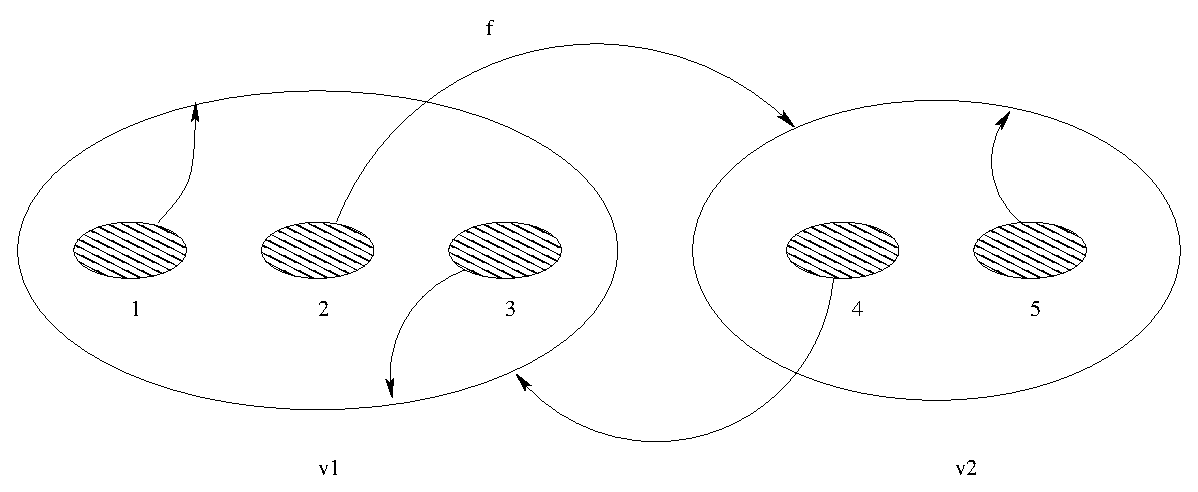
\includegraphics[scale=0.55]{cantor1.eps}
    %  note that the square brace option below is only required
    %  if you intend to produce a list of illustrations
    \caption[Shortened figure caption for the list of illustrations]
      {A Cantor repeller. Long figure captions will be indented left
      and right; short ones will be centred by default.}
    \label{cantor}
\rule[-20pt]{\textwidth}{0.6pt}
\begin{verbatim}
  \begin{figure}
    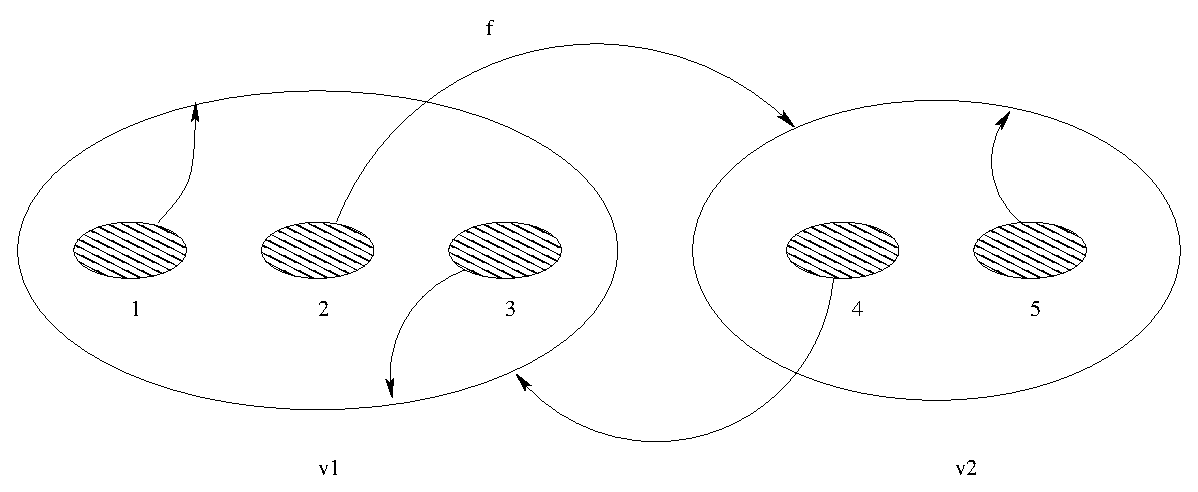
\includegraphics[scale=0.55]{cantor1.eps}
    %  note that the square brace option below is only required
    %  if you intend to produce a list of illustrations
    \caption[Shortened figure caption for the list of illustrations]
      {A Cantor repeller. Long figure captions will be indented left
      and right; short ones will be centred by default.}
    \label{cantor}
  \end{figure}
\end{verbatim}
\rule[20pt]{\textwidth}{0.5pt}
  \end{figure}

\section{Tables}

The \cambridge\ class will cope with most positioning of your tables. Table captions must be included first, the the label, then the body of the table. This is illustrated in Table~\ref{sample-table}.
  \begin{table}
    \begin{minipage}{188pt}
      %  note that the square brace option below is only required
      %  if you intend to produce a list of tables
    \caption[Shortened table caption for the list of tables]
      {Longer table captions have to be placed inside
      a minipage, otherwise they overhang the table rules.}
    \label{sample-table}
    \addtolength\tabcolsep{2pt}% to stretch columns, if required
      \begin{tabular}{@{}c@{\hspace{25pt}}ccc@{}}
        \hline \hline
        Figure\footnote{\textit{Note:} You must also use a minipage
          environment if you have footnotes.} & $hA$ & $hB$ & $hC$\\
        \hline
        1 & $\exp\left(\pi i\frac58\right)$
          & $\exp\left(\pi i\frac18\right)$ & $0$\\[3pt]
        2 & $-1$    & $\exp\left(\pi i\frac34\right)$ & $1$\\[11pt]
        3 & $-4+3i$ & $-4+3i$ & $\frac74$\\[3pt]
        4 & $-2$    & $-2$    & $\frac54 i$ \\
        \hline \hline
      \end{tabular}
    \end{minipage}
    \rule[-20pt]{\textwidth}{0.5pt}
\begin{verbatim}
  \begin{table}
    \begin{minipage}{188pt}
      %  note that the square brace option below is only required
      %  if you intend to produce a list of tables
    \caption[Shortened table caption for the list of tables]
      {Longer table captions have to be placed inside
      a minipage, otherwise they overhang the table rules.}
    \label{sample-table}
    \addtolength\tabcolsep{2pt}% to stretch columns, if required
      \begin{tabular}{@{}c@{\hspace{25pt}}ccc@{}}
        \hline \hline
        Figure\footnote{\textit{Note:} You must also use a minipage
          environment if you have footnotes.} & $hA$ & $hB$ & $hC$\\
        \hline
        1 & $\exp\left(\pi i\frac58\right)$
          & $\exp\left(\pi i\frac18\right)$ & $0$\\[3pt]
        2 & $-1$    & $\exp\left(\pi i\frac34\right)$ & $1$\\[11pt]
        3 & $-4+3i$ & $-4+3i$ & $\frac74$\\[3pt]
        4 & $-2$    & $-2$    & $\frac54 i$ \\
        \hline \hline
      \end{tabular}
    \end{minipage}
  \end{table}
\end{verbatim}
\rule[20pt]{\textwidth}{0.5pt}
  \end{table}

\subsection{My vertical rules have disappeared}

Vertical rules in tables are not \cambridge\ style, and have been automatically removed; this gives your document a truly professional look. Instead of vertical rules, we recommend the use of extra horizontal space, see Section~\ref{addhoriz}. The rules have been removed by redefining the \verb"tabular" environment. The amended definition also inserts extra vertical space above and below the horizontal rules (produced by \verb"\hline").

If you really must have them reinstated, read Section~\ref{reinstate}.

\subsection{Reinstating the vertical rules}
\label{reinstate}
Authors can revert to the standard \LaTeX\ style, if necessary. Tables will take on a rather squashed appearance, as in the \LaTeX\ book, whereby there is no added space around horizontal rules. Add the command \verb"\reinstaterules" in the preamble, and re-run your files through \LaTeX.

\subsection{There is very little space around the rules in my~table}
Tables revert to the standard, rather squashed look of standard \LaTeX\ tables for two reasons:
\begin{enumerate}
  \item you are using \verb"array.sty"; or
  \item you have chosen to reinstate vertical rules (see Section~\ref{reinstate})
\end{enumerate}
In both cases, the tabular environment is redefined.


\subsection{Adding space between columns}
\label{addhoriz}
You can add space (2pt in this example) between every column using\linebreak \verb"\addtolength\tabcolsep{2pt}". However, if you only wanted to expand the space between columns~1 and~2 to~25pt, you would do this using\linebreak  \verb"\begin{tabular}{@{}c@{\hspace{25pt}}ccc@{}}" (see Table~\ref{sample-table}).

\subsection{Adding space between rows}
If you need some form of separation between rows (for example, between rows~2 and~3 in the body of Table~\ref{sample-table}), adding \verb"[11pt]" immediately after the double backslash at the end of row~2 will add an 11pt vertical space (the equivalent of a blank line at this typesize). This is neater than adding another horizontal line.


\section{Landscape figures and tables, using rotating.sty}

Landscape figures and tables (floats) may be typeset using the \verb"rotating.sty" package. Note that the direction of rotation depends on the page number -- which requires at least two passes through \LaTeX. If we are going to know whether pages are odd or even, we need to use the \verb"\pageref" mechanism, and labels. But labels won't work unless the user has put in a caption. \textit{Beware!}

In addition to \verb"rotating.sty", you should also include \verb"floatpag.sty" and the command \verb"\rotfloatpagestyle{empty}". This combination ensures that headers and footers are removed from the float page:
\begin{verbatim}
  \usepackage{rotating}
  \usepackage{floatpag}
  \rotfloatpagestyle{empty}
\end{verbatim}
In some DVI previewers, floats may not appear rotated. If this happens, you need to convert the DVI file to PostScript or PDF.

Occasionally, when you convert a PostScript file to a PDF file, you may find that the page comes out upside-down. There will be a setting to change this. For instance, if you are using PDFCreator 0.9.7, choose the following options in this sequence:
\begin{description}
  \item Options -- Program -- PDF -- Auto-Rotate Pages: Change to `None'.
\end{description}
Other programs will have similar\vadjust{\pagebreak} procedures.


\subsection{Coding for landscape figures}

The landscape figure (Figure~\ref{sidecantor}) was typeset using the following coding:
\begin{verbatim}
  \begin{sidewaysfigure}
    \centering
    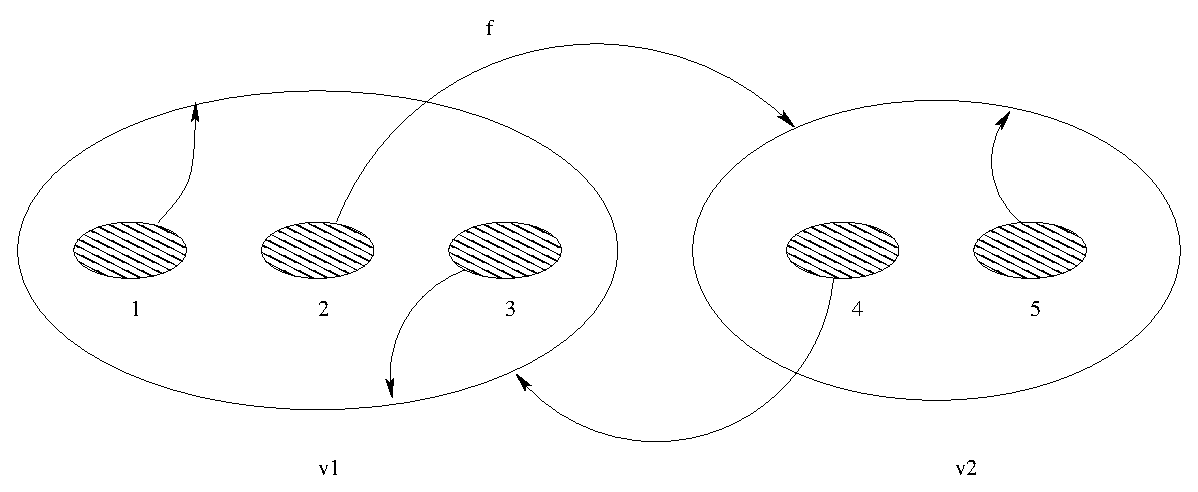
\includegraphics[scale=0.95]{cantor1.eps}
    %  note that the square brace option below is only required
    %  if you intend to produce a list of illustrations
    \caption[Landscape figure]{A Cantor repeller. Figure captions
      will be centred by default.}
    \label{sidecantor}
  \end{sidewaysfigure}
\end{verbatim}
  \begin{sidewaysfigure}
    \centering
    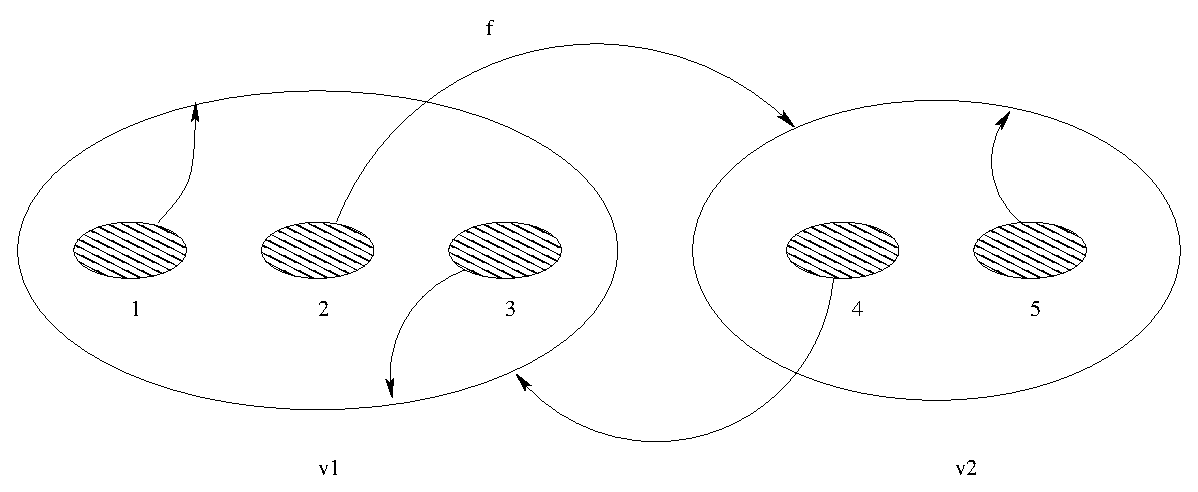
\includegraphics[scale=0.95]{cantor1.eps}
    %  note that the square brace option below is only required
    %  if you intend to produce a list of illustrations
    \caption[Landscape figure]{A Cantor repeller. Figure captions
      will be centred by default.}
    \label{sidecantor}
  \end{sidewaysfigure}



\subsection{Coding for landscape tables}

Table~\ref{sideways} has been produced using the following coding:
%
\begin{smallverbatim}
\begin{sidewaystable}
  \caption[Landscape table]{Grooved ware and beaker features, their finds and
    radiocarbon dates. For a breakdown of the pottery assemblages see
    Tables~I and~III; for the flints see Tables~II and~IV; for the animal
    bones see Table~V.}
  \label{sideways}
  \addtolength\tabcolsep{-2pt}
  \begin{tabular}{@{}lcccllccccc@{}}
  \hline\hline
  Context & Length & Breadth/  & Depth & Profile & Pottery & Flint & Animal
                                                   & Stone & Other & C14 Dates\\
  && Diameter &&&&& Bones\\[5pt]
  & m & m & m\\
  \hline\\[-5pt]
  \multicolumn{10}{@{}l}{\textbf{Grooved Ware}}\\
  784 & --   & 0.9$\phantom{0}$ &0.18  & Sloping U & P1      & $\times$46
        & $\phantom{0}$$\times$8 && $\times$2 bone & 2150 $\pm$100\,\textsc{bc}\\
  785 & --   & 1.00             &0.12   & Sloping U & P2--4  & $\times$23
                                           & $\times$21 & Hammerstone & -- & --\\
  962 & --   & 1.37             &0.20   & Sloping U & P5--6  & $\times$48
                     & $\times$57 & --& --& 1990 $\pm$80\,\textsc{bc} (Layer 4)\\
  &&&&&&&&&& 1870 $\pm$90\,\textsc{bc} (Layer 1)\\
  983 & 0.83 & 0.73             &0.25   & Stepped U & --     & $\times$18
                                & $\phantom{0}$$\times$8 & -- & Fired clay & --\\
  &&&&&&&&&&\\
  \multicolumn{10}{@{}l}{\textbf{Beaker}}\\
  552 & --   & 0.68             & 0.12  & Saucer    & P7--14 & --           & --
                                                                   & -- &-- &--\\
  790 & --   & 0.60             & 0.25  & U         & P15    & $\times$12   & --
                                                      & Quartzite-lump & -- &--\\
  794 & 2.89 & 0.75             & 0.25  & Irreg.    & P16    & $\phantom{0}$$\times$3
                                                              & -- & -- &-- &--\\
  \hline\hline
  \end{tabular}
\end{sidewaystable}
\end{smallverbatim}
%
\begin{sidewaystable}
  \caption[Landscape table]{Grooved ware and beaker features, their finds and
    radiocarbon dates. For a breakdown of the pottery assemblages see
    Tables~I and~III; for the flints see Tables~II and~IV; for the animal
    bones see Table~V.}
  \label{sideways}
  \addtolength\tabcolsep{-2pt}
  \begin{tabular}{@{}lcccllccccc@{}}
  \hline\hline
  Context & Length & Breadth/  & Depth & Profile & Pottery & Flint & Animal
                                                   & Stone & Other & C14 Dates\\
  && Diameter &&&&& Bones\\[5pt]
  & m & m & m\\
  \hline\\[-5pt]
  \multicolumn{10}{@{}l}{\textbf{Grooved Ware}}\\
  784 & --   & 0.9$\phantom{0}$ &0.18  & Sloping U & P1      & $\times$46
        & $\phantom{0}$$\times$8 && $\times$2 bone & 2150 $\pm$100\,\textsc{bc}\\
  785 & --   & 1.00             &0.12   & Sloping U & P2--4  & $\times$23
                                           & $\times$21 & Hammerstone & -- & --\\
  962 & --   & 1.37             &0.20   & Sloping U & P5--6  & $\times$48
                     & $\times$57 & --& --& 1990 $\pm$80\,\textsc{bc} (Layer 4)\\
  &&&&&&&&&& 1870 $\pm$90\,\textsc{bc} (Layer 1)\\
  983 & 0.83 & 0.73             &0.25   & Stepped U & --     & $\times$18
                                & $\phantom{0}$$\times$8 & -- & Fired clay & --\\
  &&&&&&&&&&\\
  \multicolumn{10}{@{}l}{\textbf{Beaker}}\\
  552 & --   & 0.68             & 0.12  & Saucer    & P7--14 & --           & --
                                                                   & -- &-- &--\\
  790 & --   & 0.60             & 0.25  & U         & P15    & $\times$12   & --
                                                      & Quartzite-lump & -- &--\\
  794 & 2.89 & 0.75             & 0.25  & Irreg.    & P16    & $\phantom{0}$$\times$3
                                                              & -- & -- &-- &--\\
  \hline\hline
  \end{tabular}%
\end{sidewaystable}

\endinput% features of the \cambridge\ class file
  % chap3.tex
% 2010/09/09, v2.10

\chapter{Mathematical solutions}
\label{mathsol}

\section{Why are we using amsthm.sty?}

Many authors are already using this style file, so we have decided that rather than re-invent the wheel, we will make it part of our distribution. This means that at the top of the root file must include the following lines:\\[0.5\baselineskip]
\verb"  \documentclass{"\texttt{\cambridge}\verb"}"\\
\verb"  \usepackage{amsmath}"\\
\verb"  \usepackage{amsthm}"\\[0.5\baselineskip]
As mentioned in Chapter~\ref{intro}, if your book does not use theorems, proofs, etc., then there is no need to include the amsthm package, but you do need to include these files to run this guide through \LaTeX. Note that if you are also using \verb"amsmath.sty", it \emph{must} precede \verb"amsthm.sty".

The instructions for amsthm.sty are documentated separately in \texttt{amsthdoc.pdf}. We are including \texttt{amsthm.sty} and \texttt{amsthdoc.pdf} in this distribution for your convenience, but you may find more recent versions on the web. The following sections discuss the basic features, plus a few extras.

To save time, you may cut and paste the code in Appendix~\ref{amsthmcommands} into your root file. This is a comprehensive (but not necessarily a complete) list of theorem-like environments you may wish to use.

The \verb"amsthm" commands used in this guide are detailed in Appendix~\ref{rootfile}. They are simply a subset of commands from Appendix~\ref{amsthmcommands}; some illustrate unnumbered versions.

Please note that theorems, definitions, remarks, etc.\ should be numbered in a single sequence, either by chapter (Chapter~4 would have Definition~4.1, Lemma~4.2, Lemma~4.3, Proposition~4.4, Corollary~4.5) or by section (Definition~4.1.1, Lemma~4.1.2, Lemma~4.1.3, Proposition~4.1.4, Corollary~4.1.5).

To number these elements by chapter in this guide, we have used\linebreak \verb"\newtheorem{theorem}{Theorem}[chapter]". If you prefer to have the elements numbered by section, replace \verb"[chapter]" with \verb"[section]".

\section{amsthm styles}

If no \verb"\theoremstyle" command is given, the style used will be \texttt{plain}. To specify different styles, divide your \verb"\newtheorem" commands into groups and preface each group with the appropriate \verb"\theoremstyle".

\subsection{amsthm {\upshape\texttt{plain}} style}

The \texttt{plain} style is normally used for theorems, lemmas, corollaries, propositions, conjectures, criterion and algorithms. Authors are free to define their preferred numbering systems for these. The following example resets the theorem numbers for each chapter; lemmas follow in the same sequence. We have also requested that corollaries remain unnumbered by using the starred version:
\begin{verbatim}
  \theoremstyle{plain}% default
  \newtheorem{theorem}{Theorem}[chapter]
  \newtheorem{lemma}[theorem]{Lemma}
  \newtheorem*{corollary}{Corollary}

  \begin{theorem}
    Let the scalar function\ldots
  \end{theorem}
  \begin{lemma}[Tranah]
    The first-order free surface amplitudes\ldots
  \end{lemma}
  \begin{lemma}[\citealp{MenshEst}]
    The exotic behaviours of Lagrangian\ldots
  \end{lemma}
  \begin{corollary}
    Let $G$ be the free group on\ldots
  \end{corollary}
\end{verbatim}
will produce the following output:
  \begin{theorem}
    Let the scalar function\ldots
  \end{theorem}
  \begin{lemma}[Tranah]
    The first-order free surface amplitudes\ldots
  \end{lemma}
  \begin{lemma}[\citealp{MenshEst}]
    The exotic behaviours of Lagrangian\ldots
  \end{lemma}
  \begin{corollary}
    Let $G$ be the free group on\ldots
  \end{corollary}
%
Note that Corollaries would normally be in the same numbering sequence as Theorems and Lemmas. If you'd prefer your theorems to be typeset in roman (though this is not recommended) use the amsthm \texttt{definition} style instead (see Section~\ref{amsdefn}).

\subsection{amsthm {\upshape\texttt{definition}} style}
\label{amsdefn}

The \texttt{definition} style is normally used for definitions, conditions, problems, examples. It may also be used to set up Exercises (see Appendix~\ref{amsthmcommands} for an example), although the \verb"{exerciselist}" environment described in Section~\ref{exendofsections} does the equivalent.  Again, authors are free to define their preferred numbering systems for these. However, it is most usual to continue with the same numbering sequence as for Theorems, Lemmas, etc.:
\begin{verbatim}
  \theoremstyle{definition}
  \newtheorem{definition}[theorem]{Definition}
  \newtheorem{example}[theorem]{Example}

  \begin{definition}
    The series above is the Green function\ldots
  \end{definition}
  \begin{definition}
    The correlation between the real and estimated flow\ldots
  \end{definition}
  \begin{example}
    Consider spatial and temporal problems\ldots
  \end{example}
\end{verbatim}
will produce the following output:
  \begin{definition}
    The series above is the Green function\ldots
  \end{definition}
  \begin{definition}
    The correlation between the real and estimated flow\ldots
  \end{definition}
  \begin{example}
    Consider spatial and temporal problems\ldots
  \end{example}


\subsection{amsthm {\upshape\texttt{remark}} style}
The \texttt{remark} style is normally used for remarks, notes, notation, claims, summary, acknowledgements, cases, conclusions. Again, authors are free to define their preferred numbering systems for these.
\begin{verbatim}
  \theoremstyle{remark}
  \newtheorem*{remark}{Remark}
  \newtheorem*{case}{Case}

  \begin{remark}
    The absolute amplitude of a stratified wake\ldots
  \end{remark}
  \begin{case}
    The profiles of quadratic fluctuations\ldots
  \end{case}
\end{verbatim}
will produce the following output:
  \begin{remark}
    The absolute amplitude of a stratified wake\ldots
  \end{remark}
  \begin{case}
    The profiles of quadratic fluctuations\ldots
  \end{case}

\section{Proofs}
\label{proofs}

The \verb"proof" environment is also part of the amsthm package, and provides a consistent format for proofs.
 For example,
\begin{verbatim}
  \begin{proof}
    Use $K_\lambda$ and $S_\lambda$ to translate combinators
    into $\lambda$-terms. For the converse, translate
    $\lambda x$ \ldots by [$x$] \ldots and use induction
    and the lemma.
  \end{proof}
\end{verbatim}
produces the following:
  \begin{proof}
    Use $K_\lambda$ and $S_\lambda$ to translate combinators
    into $\lambda$-terms. For the converse, translate
    $\lambda x$ \ldots by [$x$] \ldots and use induction
    and the lemma.
  \end{proof}

\subsection{Changing the word `Proof' to something else}

An optional argument allows you to substitute a different name for the standard `Proof'. To change the proof heading to read `Proof of the Pythagorean Theorem', key the following:
\begin{verbatim}
  \begin{proof}[Proof of the Pythagorean Theorem]
    Start with a generic right-angled triangle\ldots
  \end{proof}
\end{verbatim}
which produces:
  \begin{proof}[Proof of the Pythagorean Theorem]
    Start with a generic right-angled triangle\ldots
  \end{proof}


\subsection{Typesetting a proof without a \qedsymbol}

This is not part of the amsthm package. Use the \verb"proof*" version. For example,
\begin{verbatim}
  \begin{proof*}
    The apparent virtual mass coefficient\ldots
  \end{proof*}
\end{verbatim}
produces the following:
  \begin{proof*}
    The apparent virtual mass coefficient\ldots
  \end{proof*}

\subsection{Placing the \qedsymbol\ after a displayed equation}

To avoid the \qedsymbol\ dropping onto the following line at the end of a proof,
\begin{verbatim}
  \begin{proof}
    \ldots and, as we are all aware,
    \[
       E=mc^2. \qedhere
    \]
  \end{proof}
\end{verbatim}
produces the following:
  \begin{proof}
    \ldots and, as we are all aware,
    \[
       E=mc^2. \qedhere
    \]
  \end{proof}
When used with the amsmath package, version~2 or later, \verb"\qedhere" will position \qedsymbol\ flush right; with earlier versions, \qedsymbol\ will be spaced a quad away
from the end of the text or display.

If \verb"\qedhere" produces an error message in an equation, try using \verb"\mbox{\qedhere}" instead.

\subsection{Placing the \qedsymbol\ after a displayed eqnarray}

This is also not part of the amsthm package. To enable this, you need to used the starred version of \verb"proof", and add both \verb"\arrayqed" and \verb"\arrayqedhere", as shown in the following example:
\begin{verbatim}
  \begin{proof*}
    The following equations prove the theorem:
      \arrayqed
        \begin{eqnarray}
          \epsilon &=& -\frac{1}{2}U_0\frac{\mathrm{d}q'^2}
                       {\mathrm{d}x}\nonumber\\
                   &=& 10\nu\frac{q'^2}{\lambda^2}
        \arrayqedhere
        \end{eqnarray}
  \end{proof*}
\end{verbatim}
produces the following:
  \begin{proof*}
    The following equations prove the theorem:
      \arrayqed
        \begin{eqnarray}
          \epsilon &=& -\frac{1}{2}U_0\frac{\mathrm{d}q'^2}
                       {\mathrm{d}x}\nonumber\\
                   &=& 10\nu\frac{q'^2}{\lambda^2}
        \arrayqedhere
        \end{eqnarray}
  \end{proof*}

\endinput
% mathematical solutions

  \part{Closing features}
  % chap4.tex
% 2010/09/09, v2.10

\chapter{Reference and bibliography lists}

\section{Automatic lists using \textsc{Bib}\upshape{\TeX}}

We have chosen to use the natbib package because of its versatility.

First, call in \texttt{natbib.sty}. If you are using the multi-contributor option, you will get an unnumbered section heading, otherwise it will be an unnumbered chapter heading.

The bibliography file for this guide (\texttt{\cambridge guide.tex}) is called \texttt{percolation.bib}; the bibliography style is \texttt{cambridgeauthordate.bst}, so place the final two commands at the point where you would like the references to appear:
%
\begin{verbatim}
    \usepackage{natbib}
      :
  % \renewcommand{\refname}{Bibliography}
    \bibliography{percolation}
    \bibliographystyle{cambridgeauthordate}
\end{verbatim}
%
Note that if you uncomment the third line shown above, you can change the heading from `References' to `Bibliography'. Next, \LaTeX\ your book twice. Then run \textsc{Bib}\TeX\ by executing the command\\[0.5\baselineskip]
\verb"  bibtex "\texttt{\cambridge guide}\\[0.5\baselineskip]
Finally, run your book through \LaTeX\ twice again. This series of runs will generate a file called \texttt{\cambridge guide.bbl}, which will then be included by \verb"\bibliography{percolation}".

Suppose you have cited 8 entries from the `percolation' database, e.g. \verb"\citealp{MenshEst}"; \verb"\citealp{Kasymp}"; \verb"\citealp{VGFH}"; \verb"\citealp{HamMaz94}"; \verb"\citealp{HamLower}"; \verb"\citealp{AiBar87}"; \verb"\citealp{MMS}"; and \verb"\citealp{HamAtomBond}"; the output will be just those 8~entries (see page~\pageref{refs}).%
% add these entries to the list without referring to them
\nocite{MenshEst}\nocite{Kasymp}\nocite{VGFH}\nocite{HamMaz94}\nocite{HamLower}\nocite{AiBar87}\nocite{MMS}\nocite{HamAtomBond}

\section{Citations using natbib commands}
Here are some of the basic citation commands available with the natbib package; there are many more if you cannot find what you need in this list. Bear in mind that Menshikov (1985) or (Menshikov, 1985) read best, depending on context.\\*[0.5\baselineskip]
\begin{tabular}{@{}ll@{}}
\verb"\citep{MenshEst}"
    & $\rightarrow\enskip$\citep{MenshEst}\\
\verb"\citep[see][p.$\,$34]{MenshEst}"
    & $\rightarrow\enskip$\citep[see][p.$\,$34]{MenshEst}\\
\verb"\citep[e.g.][]{MenshEst}"
    & $\rightarrow\enskip$\citep[e.g.][]{MenshEst}\\
\verb"\citep[Section~2.3]{MenshEst}"
    & $\rightarrow\enskip$\citep[Section~2.3]{MenshEst}\\
\verb"\citep{MenshEst, VGFH}"\\
    & $\hspace{-70pt}\rightarrow\enskip$\citep{MenshEst, VGFH}\\
\verb"\cite{MenshEst, VGFH}"\\
    & $\hspace{-70pt}\rightarrow\enskip$\cite{MenshEst, VGFH}\\
\verb"\citealt{MenshEst}"
    & $\rightarrow\enskip$\citealt{MenshEst}\\
\verb"\cite{MenshEst}"
    & $\rightarrow\enskip$\cite{MenshEst}\\
\verb"\citealp{MenshEst}"
    & $\rightarrow\enskip$\citealp{MenshEst}\\
\verb"\citeauthor{MenshEst}"
    & $\rightarrow\enskip$\citeauthor{MenshEst}\\
\verb"\citeyearpar{MenshEst}"
    & $\rightarrow\enskip$\citeyearpar{MenshEst}\\
\verb"\citeyear{MenshEst}"
    & $\rightarrow\enskip$\citeyear{MenshEst}
\end{tabular}


\section{How to change reference entries from author--date to~numbers}
\label{numberedbiblio}

\LaTeX\ authors are used to \verb"\cite{...}" producing a reference such as~[11] in their manuscripts. If you prefer this style, it is an option within the natbib package:
\begin{verbatim}
  \usepackage[numbers]{natbib}
\end{verbatim}

\section{Keying in your reference list for an author--date system}
\label{authordatebiblio}

The entries need to be keyed as below. Note that if you uncomment the first line, you can change the heading from `References' to `Bibliography':
%
\begin{smallverbatim}
% \renewcommand{\refname}{Bibliography}
  \begin{thebibliography}{8}
    \expandafter\ifx\csname natexlab\endcsname\relax
      \def\natexlab#1{#1}\fi
    \expandafter\ifx\csname selectlanguage\endcsname\relax
      \def\selectlanguage#1{\relax}\fi

  \bibitem[Aizenman and Barsky, 1987]{AiBar87}
    Aizenman, M., and Barsky, D.~J. 1987.
    Sharpness of the phase transition in percolation models.
    {\em Comm. Math. Phys.}, {\bf 108}, 489--526.

  \bibitem[Hammersley, 1957]{HamLower}
    Hammersley, J.~M. 1957.
    Percolation processes: Lower bounds for the critical probability.
    {\em Ann. Math. Statist.}, {\bf 28}, 790--795.

  \bibitem[Hammersley, 1961]{HamAtomBond}
    Hammersley, J.~M. 1961.
    Comparison of atom and bond percolation processes.
    {\em J. Mathematical Phys.}, {\bf 2}, 728--733.

  \bibitem[Hammersley and Mazzarino, 1994]{HamMaz94}
    Hammersley, J.~M., and Mazzarino, G. 1994.
    Properties of large Eden clusters in the plane.
    {\em Combin. Probab. Comput.}, {\bf 3}, 471--505.

  \bibitem[Kesten, 1990]{Kasymp}
    Kesten, H. 1990.
    Asymptotics in high dimensions for percolation.
    Pages  219--240 of: Grimmett, G.~R., and Welsh, D.~J.~A. (eds),
    {\em Disorder in Physical Systems: A Volume in Honour of John Hammersley}.
    Oxford University Press.

  \bibitem[Menshikov, 1985]{MenshEst}
    Menshikov, M.~V. 1985.
    Estimates for percolation thresholds for lattices in {${\bf R}\sp n$}.
    {\em Dokl. Akad. Nauk SSSR}, {\bf 284}, 36--39.

  \bibitem[Menshikov et~al., 1986]{MMS}
    Menshikov, M.~V., Molchanov, S.~A., and Sidorenko, A.~F. 1986.
    Percolation theory and some applications.
    Pages  53--110 of: {\em Probability theory. Mathematical
    statistics. Theoretical cybernetics, Vol. 24 (Russian)}.
    Akad. Nauk SSSR Vsesoyuz. Inst. Nauchn. i Tekhn. Inform.
    Translated in {\em J. Soviet Math}. {\bf 42} (1988), no. 4,
    1766--1810.

  \bibitem[Vyssotsky et~al., 1961]{VGFH}
    Vyssotsky, V.~A., Gordon, S.~B., Frisch, H.~L., and Hammersley, J.~M. 1961.
    Critical percolation probabilities (bond problem).
    {\em Phys. Rev.}, {\bf 123}, 1566--1567.

  \end{thebibliography}
\end{smallverbatim}

\section{Keying in your reference list for a numbered system}

For this style, you may omit the optional square brace shown in Section~\ref{authordatebiblio}. Once again, if you uncomment the first line, you can change the heading from `References' to `Bibliography':
%
\begin{smallverbatim}
% \renewcommand{\refname}{Bibliography}
  \begin{thebibliography}{8}

  \bibitem{AiBar87}
    Aizenman, M., and Barsky, D.~J. 1987.
    Sharpness of the phase transition in percolation models.
    {\em Comm. Math. Phys.}, {\bf 108}, 489--526.

  \bibitem{HamLower}
    Hammersley, J.~M. 1957.
    Percolation processes: Lower bounds for the critical probability.
    {\em Ann. Math. Statist.}, {\bf 28}, 790--795.

  \bibitem{HamAtomBond}
    Hammersley, J.~M. 1961.
    Comparison of atom and bond percolation processes.
    {\em J. Mathematical Phys.}, {\bf 2}, 728--733.
      :
      :
  \bibitem[Vyssotsky et~al., 1961]{VGFH}
    Vyssotsky, V.~A., Gordon, S.~B., Frisch, H.~L., and Hammersley, J.~M. 1961.
    Critical percolation probabilities (bond problem).
    {\em Phys. Rev.}, {\bf 123}, 1566--1567.

  \end{thebibliography}
\end{smallverbatim}

\endinput% references and bibliographies
  % chap5.tex
% 2010/09/09, v2.10

\chapter{Indexes}
\label{indexes}

\section{Creating a single index using makeidx.sty}
To generate a single index, normally a subject index, the commands would take the form:
\begin{verbatim}
  \index{diffraction}
  \index{force!hydrodynamic}
  \index{force!interactive}
\end{verbatim}
  %\index{diffraction}%
  %\index{force!hydrodynamic}%
  %\index{force!interactive}%
The following commands are then required in the preamble:
\begin{verbatim}
  \usepackage{makeidx}
  \makeindex
\end{verbatim}
and at the point you wish your index to appear,
\begin{verbatim}
  \printindex
\end{verbatim}
Run your book through \LaTeX\ enough times so that the labels, etc., are stable. Then execute the command:\\[0.5\baselineskip]
\verb"  makeindex "\texttt{\cambridge guide}\\[0.5\baselineskip]
To include the index, you need to run \LaTeX\ one more time.


\section{Creating multiple indexes using multind.sty}
This guide has been prepared using \verb"multind.sty". This style file redefines the \verb"\makeindex", \verb"\index" and \verb"\printindex" commands to deal with multiple indexes.

Suppose you want to create an author index and a subject index. The entries should be in the text as usual, but take the following form:
\begin{verbatim}
  \index{authors}{Young, P.D.F.}
  \index{authors}{Tranah, D.A.}
  \index{authors}{Peterson, K.}
  \index{subject}{diffraction}
  \index{subject}{force!hydrodynamic}
  \index{subject}{force!interactive}
\end{verbatim}
  \index{authors}{Young, P.D.F.}%
  \index{authors}{Tranah, D.A.}%
  \index{authors}{Peterson, K.}%
  \index{subject}{diffraction}%
  \index{subject}{force!hydrodynamic}%
  \index{subject}{force!interactive}%
In the preamble, you need to add the following lines:
\begin{verbatim}
  \usepackage{multind}\ProvidesPackage{multind}
  \makeindex{authors}
  \makeindex{subject}
\end{verbatim}
It is crucial to add the command \verb"\ProvidesPackage{multind}"; this will send a message to the class file to re-style the index into the \cambridge\ style. You will get a warning in your log file:
\begin{verbatim}
  LaTeX Warning: You have requested package `',
                 but the package provides `multind'.
\end{verbatim}
which can be ignored. At the point where you wish your indexes to appear, you then need the commands:
\begin{verbatim}
  \printindex{authors}{Author index}
  \printindex{subject}{Subject index}
\end{verbatim}
Run your book through \LaTeX\ enough times so that the labels, etc., are stable. Then execute the commands:
\begin{verbatim}
  makeindex authors
  makeindex subject
\end{verbatim}
To include the indexes, you need to run \LaTeX\ one more time.

\section{Creating multiple indexes using index.sty}

This style file allows you to define new indexes. Suppose you want to create an author index as well as a normal subject index. The entries should be in the text as usual, but take the following form:
\begin{verbatim}
  \index[aut]{Young, P.D.F.}
  \index[aut]{Tranah, D.A.}
  \index[aut]{Peterson, K.}
  \index{diffraction}
  \index{force!hydrodynamic}
  \index{force!interactive}
\end{verbatim}
  %\index[aut]{Young, P.D.F.}%
  %\index[aut]{Tranah, D.A.}%
  %\index[aut]{Peterson, K.}
  %\index{diffraction}%
  %\index{force!hydrodynamic}%
  %\index{force!interactive}%
To create the extra author index, you need to have the following lines in the preamble:
\begin{verbatim}
  \usepackage{index}
  \makeindex
  \newindex{aut}{adx}{and}{Author index}
\end{verbatim}
At the point where you wish your indexes to appear, use:
\begin{verbatim}
  \printindex[aut]
  \printindex
\end{verbatim}
Run your book through \LaTeX\ enough times so that the labels, etc., are stable. Then execute the commands:\\[0.5\baselineskip]
\verb"  makeindex -o "\texttt{\cambridge guide.and \cambridge guide.adx}\\
\verb"  makeindex "\texttt{\cambridge guide}\\[0.5\baselineskip]
To include the indexes, you need to run \LaTeX\ one more time.

\subsection{Caution -- from the authors of index.sty}

In order to implement \verb"index.sty", it's been necessary to modify a number of \LaTeX\ commands seemingly unrelated to indexing, namely, \verb"\@starttoc", \verb"\raggedbottom", \verb"\flushbottom", \verb"\addcontents", \verb"\markboth", and \verb"\markright". Naturally, this could cause incompatibilities between \texttt{index.sty} and any style files that either redefine these same commands or make specific assumptions about how they operate.

The redefinition of \verb"\@starttoc" is particularly bad, since it introduces an incompatibility with the AMS document classes. This will be addressed soon.

In the current implementation, \texttt{index.sty} uses one output stream for each index.  Since there are a limited number of output indexes, this means that there is a limit on the number of indexes you can have in a document.  There is more information on this in \verb"index.dtx" which is part of the \verb"index.sty" distribution.\\[\baselineskip]
%
\textit{For these reasons, whilst all care has been taken to deal with these changes in \cambridge.cls, if you do find incompatibilities with other files, please contact us at texline@cambridge.org with your source files, class and style files, and log file.}

\endinput
% single and multiple indexes

  \backmatter
% if you only have one appendix, use \oneappendix instead of \appendix
  \appendix
  % appendixA.tex
% 2010/09/09, v2.10

\chapter{Typesetting appendices}

\section{Single-contributor books}
\subsection{How to typeset one appendix}
If you have just one appendix, say \verb"appendix.tex", you will want to generate a chapter head `Appendix' rather than `Appendix A'. Use \verb"\oneappendix" in the main file, as follows:
\begin{verbatim}
  \oneappendix
  \include{appendix}
\end{verbatim}

\subsection{How to typeset several appendices}
The coding used to generate the appendices in this guide is as follows:
\begin{verbatim}
  \appendix
  \include{appendixA}
  \include{appendixB}
  \include{appendixC}
\end{verbatim}

\section{Multi-contributor books}

\subsection{How to typeset one appendix}
If you have just one appendix, it will be the next section head and you should include the following code at the end of your chapter:
\begin{verbatim}
  \oneappendix
  \section{Appendix heading}
  \subsection{Subheading}
  \endappendix
\end{verbatim}
You will need to add \verb"\endappendix" if you have further section heads in this chapter.


\subsection{How to typeset several appendices}
The following code will genenerate Appendix~A and Appendix~B at the end of your chapter:
\begin{verbatim}
  \appendix
  \section{Appendix heading}
  \subsection{Subheading}
    :
  \section{Next appendix heading}
  \subsection{Next subheading}
  \endappendix
\end{verbatim}
Again, you will need to add \verb"\endappendix" if you have further section heads in this chapter.

\section{Numbering systems}

Equations in appendices will be numbered as follows:
\begin{equation}
  E=mc^2,
\end{equation}
and figure captions as follows:
\begin{figure}[h]
\caption[Similarity solutions]{Similarity solutions.}
\end{figure}

\endinput
  % appendixB.tex
% 2010/09/09, v2.10

\chapter{amsthm commands}
\label{amsthmcommands}

The following code may be cut and pasted into your root file. Assuming you have included \verb"amsthm.sty", it will number your theorems, definitions, etc. in the same numbering sequence and by chapter, e.g.~Definition~4.1, Lemma~4.2, Lemma~4.3, Proposition~4.4, Corollary~4.5.

If you prefer to have the elements numbered by section, e.g.~Definition~4.1.1, Lemma~4.1.2, Lemma~4.1.3, Proposition~4.1.4, Corollary~4.1.5, replace \verb"[chapter]" on line 2 with \verb"[section]".

\begin{smallverbatim}

  \theoremstyle{plain}% default
  \newtheorem{theorem}{Theorem}[chapter]
  \newtheorem{lemma}[theorem]{Lemma}
  \newtheorem{corollary}[theorem]{Corollary}
  \newtheorem{proposition}[theorem]{Proposition}
  \newtheorem{conjecture}[theorem]{Conjecture}
  \newtheorem{criterion}[theorem]{Criterion}
  \newtheorem{algorithm}[theorem]{Algorithm}

  \theoremstyle{definition}
  \newtheorem{definition}[theorem]{Definition}
  \newtheorem{condition}[theorem]{Condition}
  \newtheorem{problem}[theorem]{Problem}
  \newtheorem{example}[theorem]{Example}
  \newtheorem{exer}{Exercise}[section]
    % note that {exer} may be used for Exercises scattered
    % throughout a chapter;
    %   - they will be numbered by [section]
    %   - we have not used {exercise} as this is already defined

  \theoremstyle{remark}
  \newtheorem{remark}[theorem]{Remark}
  \newtheorem{note}[theorem]{Note}
  \newtheorem{notation}[theorem]{Notation}
  \newtheorem{claim}[theorem]{Claim}
  \newtheorem{summary}[theorem]{Summary}
  \newtheorem{acknowledgement}[theorem]{Acknowledgement}
  \newtheorem{case}[theorem]{Case}
  \newtheorem{conclusion}[theorem]{Conclusion}
\end{smallverbatim}

\endinput
  % appendixC.tex
% 2010/09/09, v2.10

\chapter{The root file for this guide}
\label{rootfile}

\begin{smallverbatim}
% cambridge6Aguide.tex
% for the suite of standard Cambridge designs
% 2010/09/09, v2.10

  \NeedsTeXFormat{LaTeX2e}[1996/06/01]

% \documentclass[multi,spanningrule]{cambridge6A}% options
  \documentclass{cambridge6A}
  \usepackage{natbib}

  \usepackage{rotating}
  \usepackage{floatpag}
  \rotfloatpagestyle{empty}

% \usepackage{amsmath}% if you are using this package,
                      % it must be loaded before amsthm.sty
  \usepackage{amsthm}
  \usepackage{graphicx}

% indexes
% uncomment the relevant set of commands

% for a single index
% \usepackage{makeidx}
% \makeindex

% for multiple indexes using multind.sty
  \usepackage{multind}\ProvidesPackage{multind}
  \makeindex{authors}
  \makeindex{subject}

% for multiple indexes using index.sty
% \usepackage{index}
% \newindex{aut}{adx}{and}{Author index}
% \makeindex

  \newcommand\cambridge{cambridge6A}

% see chapter 3 for details
  \theoremstyle{plain}% default
  \newtheorem{theorem}{Theorem}[chapter]
  \newtheorem{lemma}[theorem]{Lemma}
  \newtheorem*{corollary}{Corollary}

  \theoremstyle{definition}
  \newtheorem{definition}[theorem]{Definition}
  \newtheorem{example}[theorem]{Example}

  \theoremstyle{remark}
  \newtheorem*{remark}{Remark}
  \newtheorem*{case}{Case}

  \hyphenation{line-break line-breaks docu-ment triangle cambridge amsthdoc
    cambridgemods baseline-skip author authors cambridgestyle en-vir-on-ment polar}

  \setcounter{tocdepth}{2}% the toc normally lists sections;
% for the purposes of this document, this has been extended to subsections

%%%%%%%%%%%%%%%%%%%%%%%%%%%%%%%%%%%%%

% \includeonly{chap1}

%%%%%%%%%%%%%%%%%%%%%%%%%%%%%%%%%%%%%
  \begin{document}

  \title[Subtitle, If You Have One]
    {\LaTeXe\ GUIDE FOR AUTHORS USING THE \cambridge\ DESIGN}

  \author{Ali Woollatt\\[3\baselineskip]
    This guide was compiled using \hbox{\cambridge.cls \version}\\[\baselineskip]
    The latest version can be downloaded from:
    https://authornet.cambridge.org/information/productionguide/
      LaTeX\_files/\cambridge.zip}

  \frontmatter
  \maketitle
  \tableofcontents
  \listoffigures
  \listoftables
  \listofcontributors

  \mainmatter
  \part{Getting started}
  \include{chap1}% introduction
  \include{chap2}% features of the \cambridge\ class file
  \include{chap3}% mathematical solutions

  \part{Closing features}
  \include{chap4}% references and bibliographies
  \include{chap5}% single and multiple indexes

  \backmatter
% if you only have one appendix, use \oneappendix instead of \appendix
  \appendix
  \include{appendixA}
  \include{appendixB}
  \include{appendixC}
  \endappendix

% insert a blank line to the toc list
  \addtocontents{toc}{\vspace{\baselineskip}}
  \theendnotes

% \renewcommand{\refname}{Bibliography}% if you prefer this heading
  \bibliography{percolation}\label{refs}
  \bibliographystyle{cambridgeauthordate}

  \cleardoublepage

% indexes

% for a single index
% \printindex

% for multiple indexes using multind.sty
  \printindex{authors}{Author index}
  \printindex{subject}{Subject index}

% for multiple indexes using index.sty
% \printindex[aut]
% \printindex

\end{document}
\end{smallverbatim}

\endinput
  \endappendix

% insert a blank line to the toc list
  \addtocontents{toc}{\vspace{\baselineskip}}
  \theendnotes

% \renewcommand{\refname}{Bibliography}% if you prefer this heading
  \bibliography{percolation}\label{refs}
  \bibliographystyle{cambridgeauthordate}

  \cleardoublepage

% indexes

% for a single index
% \printindex

% for multiple indexes using multind.sty
  \printindex{authors}{Author index}
  \printindex{subject}{Subject index}

% for multiple indexes using index.sty
% \printindex[aut]
% \printindex

\end{document}
\end{smallverbatim}

\endinput
  \endappendix

% insert a blank line to the toc list
  \addtocontents{toc}{\vspace{\baselineskip}}
  \theendnotes

% \renewcommand{\refname}{Bibliography}% if you prefer this heading
  \bibliography{percolation}\label{refs}
  \bibliographystyle{cambridgeauthordate}

  \cleardoublepage

% indexes

% for a single index
% \printindex

% for multiple indexes using multind.sty
  \printindex{authors}{Author index}
  \printindex{subject}{Subject index}

% for multiple indexes using index.sty
% \printindex[aut]
% \printindex

\end{document}
\end{smallverbatim}

\endinput
\end{verbatim}

\section{Multi-contributor books}

\subsection{How to typeset one appendix}
If you have just one appendix, it will be the next section head and you should include the following code at the end of your chapter:
\begin{verbatim}
  \oneappendix
  \section{Appendix heading}
  \subsection{Subheading}
  \endappendix
\end{verbatim}
You will need to add \verb"\endappendix" if you have further section heads in this chapter.


\subsection{How to typeset several appendices}
The following code will genenerate Appendix~A and Appendix~B at the end of your chapter:
\begin{verbatim}
  \appendix
  \section{Appendix heading}
  \subsection{Subheading}
    :
  \section{Next appendix heading}
  \subsection{Next subheading}
  \endappendix
\end{verbatim}
Again, you will need to add \verb"\endappendix" if you have further section heads in this chapter.

\section{Numbering systems}

Equations in appendices will be numbered as follows:
\begin{equation}
  E=mc^2,
\end{equation}
and figure captions as follows:
\begin{figure}[h]
\caption[Similarity solutions]{Similarity solutions.}
\end{figure}

\endinput